%%%%%%%%%%%%%%%%%%%%%%%%%%%%%%%%%%%%%%%%%%%%%%%%%%%%%%%%%
%    Formato de memoria de Trabajo Final de Grado (TFG) para la Facultad de Ingeniería de la Universidad Nacional de Asunción.

%   Version 2.0.1 por Msc. Ing. Sergio Ramón Toledo Gallardo del 10 de junio de 2015                           
%- La compilación debe realizarse utilizando el comando pdflatex o pdflatexmk (para Mac)%
% Los programas necesarios son Miktex 2.9 (distribución latex) y algún procesador como el texmaks o texniccenter
%- Para texnicCenter Usar makeindex y habilitar usar bibtex
%-  Al imprimir el PDF se debe seleccionar tamaño real y Elegir origen por tamaño de pagina PDF para respetar los margenes requeridos   
%- Las figuras deben cargarse en la carpeta "imagenes" en formato pdf para optimizar la velocidad de compilación, sin embargo también se permiten formatos jpg y eps.
%- Las referencia bibliográficas se cargan en el archivo    fiuna.bib                                                       %%%%%%%%%%%%%%%%%%%%%%%%%%%%%%%%%%%%%%%%%%%%%%%%%%%%%
\documentclass[oneside, a4paper, 12pt]{fiuna}
\usepackage{fiuna}

%%%%%%%%%%%%%%%%%%%%%%%%%%%%%%%%%%%%%%%%%%%%%%%%%%%%%%%%%%
%               Inicio del documento                     %
%%%%%%%%%%%%%%%%%%%%%%%%%%%%%%%%%%%%%%%%%%%%%%%%%%%%%%%%%%
\usepackage{minted}
\usepackage{float}
\usepackage{hyperref}


\begin{document}

    %%%Introduzca el nombre de los autores
    %\autor[Nombre Corto]{Nombre completo del autor}
    \autor[Rodney Rojas]{Rodney Ruben Rojas Sosa}
    %\autor{Autor 2}
    %%%Introduzca el título del TFG
    \titulo{Dise\~no de sonda para medici\'on a multiniveles de factores fisicoqu\'imicos de recursos h\'idricos.}
    %%%introduce la carrera
    \carrera{Ingenier\'ia en Mecatr\'onica}
    %%%Nombre del Asesor del TFG %%%%%
    \asesor{Dr. Ing. Derlis Gregor}
    \asesor{Dr. Ing. Mario Arzamendia }
    %\asesor{Ing. Asesor 3}
    %%%%%%Ciudad donde se presenta%%%%%%%%%%%
    \ciudad{San Lorenzo}
    %%%%%% A quien se dedique %%%%%%%%%%%%%%
    \dedicatoria{A mi madre}
    \pagenumbering{roman}
    
    \preliminares
    
    \pagenumbering{arabic}
    \tableofcontents
    \listoffigures
    \listoftables
    %% En caso de no tener anexos comentar la siguiente linea
    \listofappendices
    \formatoTitulos
    
    %%% Inician los capítulos de la memoria de TFG%%%%
    %cada capitulo se introduce con \input
    %El primer capitulo siempre es la introducción al TFG
     % [RR] FECHA DE HOY jaja 28/09/ 20 :(


\chapter[Introducción]{Introducción}
\pagestyle{fancy}

%\section{Introducción}

El agua es un elemento \'unico de la naturaleza, \cite{caribbean_seguridad_2020} el agua dulce es un recurso natural importante e indispensable en todas las actividades sociales, económicas y ambientales, es una condición para toda la vida en nuestro planeta.
Se lo puede encontrar en la naturaleza en sus tres estados f\'isicos(sólido, l\'iquido y gaseoso), y constituye la  mayor parte de la superficie del planeta.
Hist\'oricamente, estuvimos en contacto con el agua como fuente de hidratación, medio de transporte, agricultura, ganadería, materia prima, entre otros, a medida que transcurrió el tiempo se puedo observar como este vital líquido, sufrió importantes alteraciones debido a la explotación irresponsables por las actividades humanas. 
A partir del siglo XX la humanidad ha comprendido la importancia de la conservación, analizando y estudiando como nuestras actividades impactan, pudiendo alterar un ecosistema.
Mediante pol\'iticas p\'ublicas, se busca regular varios aspectos con tratados nacionales e internacionales, con el fin de preservar los ecosistemas naturales.

Desde el a\~no 2015, los líderes mundiales adoptaron 17 Objetivos de Desarrollo Sostenible (ODS) para proteger el planeta, luchar contra la pobreza y tratar de erradicarla con el objetivo de construir un mundo más próspero,  justo y sostenible para las generaciones futuras, \cite{bbva_que_nodate}. 
Entre los objetivos de desarrollo se encuentra el agua, espec\'ificamente en el ODS 6, denominado Agua Limpia y saneamiento, cuyo objetivo es Garantizar la disponibilidad de agua y su gestión sostenible y el saneamiento para todos, a trav\'es de siete objetivos, \cite{onu_agua_nodate} 
, ODS 6.3  De aquí a 2030, mejorar la calidad del agua, reduciendo la contaminación, eliminando el vertimiento y minimizando la emisión de productos químicos y materiales peligrosos, reduciendo a la mitad el porcentaje de aguas residuales sin tratar y aumentando considerablemente el reciclado y la reutilización sin riesgos a nivel mundial
, ODS 6.5  De aquí a 2030, implementar la gestión integrada de los recursos hídricos a todos los niveles, incluso mediante la cooperación transfronteriza, según proceda
, ODS 6.6  De aquí a 2020, proteger y restablecer los ecosistemas relacionados con el agua, incluidos los bosques, las montañas, los humedales, los ríos, los acuíferos y los lagos
, ODS 6.a  De aquí a 2030, ampliar la cooperación internacional y el apoyo prestado a los países en desarrollo para la creación de capacidad en actividades y programas relativos al agua y el saneamiento, como los de captación de agua, desalinización, uso eficiente de los recursos hídricos, tratamiento de aguas residuales, reciclado y tecnologías de reutilización
, ODS 6.b  Apoyar y fortalecer la participación de las comunidades locales en la mejora de la gestión del agua y el saneamiento,\cite{moran_agua_nodate}.

La humanidad ha sido testigo de c\'omo se han perdido ecosistemas completos, extinguiéndose la fauna y flora, por la alteraci\'on de los ecosistemas a causa de la contaminaci\'on, que modifica la calidad de los suelos y recursos h\'idricos, causando da\~nos al medio ambiente y una serie de consecuencias muchas veces irreversibles.
El Paraguay es un pa\'is rico en recursos naturales, posee unos 336 km$^3$ de agua dulce dentro de su territorio. 
El acuífero Guaraní es la tercera mayor reserva de agua dulce del mundo, compartido con Brasil, Argentina y Uruguay, con 70.000 km$^{2}$ de superficie en Paraguay,\cite{stp_Agua}. 
Por ello, es de vital importancia tener e implementar políticas p\'ublicas y departamentos que protejan, regulen y preserven estos recursos.
El monitoreo de los recursos hídricos es esencial para detectar cambios y tomar las acciones requeridas a tiempo.
En el país, existen una gran cantidad de fábricas e industrias que no poseen sistemas de tratamiento de efluentes de producci\'on, vertiendo sus desechos residuales a los afluentes sin previo trabajo de depuración en planta, que no son controlados y regulados por un gran déficit de fiscalización ambiental, por las limitaciones en la mayor parte tecnol\'ogicos para poder realizar un muestreo de una forma r\'apida y confiable por los departamentos fiscalizadores competentes. 

El presente trabajo final de grado (TFG), propone el diseño y fabricación de una sonda aplicado al monitoreo de calidad del agua mediante sensores para la medición automática del potencial del hidrógeno (PH), temperatura (T), oxígeno disuelto(DO), potencial de \'oxido reducción (OPR) y conductividad eléctrica (CE). 
Par\'ametros que seg\'un estándares nacionales e internaciones, son indicadores básicos para analizar el estado del recurso hídrico y poder inferir sobre la calidad del mismo.
El TFG se enmarca en el proyecto PINV 15-177 - Vehículo Autónomo de Superficie (ASV) para el estudio de calidad del agua en lagos y lagunas, desarrollado en el Laboratorio de Sistemas Distribuido (LSD) perteneciente a la Facultad de Ingeniería de una Universidad Nacional de Asunción (FIUNA) con sede en el Centro de Innovación Tecnológica (CITEC). 
El ASV no forma parte del desarrollo de este TFG, proporciona una automatización para el muestreo, transportando la sonda hasta la locación deseada, georeferenciando los datos obtenidos y mediante una gr\'ua se amplía la capacidad de sensado a diferentes niveles de profundidad. 
Como menciona en su gu\'ia Hanna Instruments, sobre la importancia de reconocer que la calidad del agua deficiente puede afectar de manera negativa,  ya sea por razones naturales y/o por factores humanos, donde un monitoreo regular de los recursos hídricos pudiendo ayudar a identificar problemas antes de que generen algún deterioro de algún ecosistema, \cite{guiaHANNA}.
El TFG  se organiza en cinco capítulos desarrollados de la siguiente manera: 
en el capítulo uno, se presentan los objetivos generales y específicos,  un breve an\'alisis de la problemática y el alcance del trabajo realizado;
en el capítulo dos, se describen los antecedentes sobre el monitoreo de recursos hídricos y las definiciones relevantes;
en el capítulo tres, se desarrolla el diseño de las partes lo concerniente al desarrollo del sistema y la integración de todos sus componentes;   
en el cap\'itulo cuatro, se desarrolla las pruebas realizadas y resultados obtenidos con la sonda;
por último, en el capítulo cinco se presentan las conclusiones obtenidas, recomendaciones, trabajos futuros y divulgaciones.
%[RR] Yo metí todo dentro de "sistema " realmente , podria agregar una descripción mas detallada para que se entienda lo que abarca  

\section{Objetivo General}
Desarrollar una sonda y sistema de despliegue para muestreo a multinivel de factores fisicoquímicos de recursos hídricos.

\section{Objetivos Específicos} \label{Objetivos}
\begin{itemize}
	\item Dise\~nar la sonda que contendrá a los sensores de CE, pH, OD, OPR, T.
    \item Investigar la sonda en el material apto.
    % [RR] Yo primero hice el diseño para impresora 3D y después vi como fabricar, onda lo que queria es el motivo de la impresión 3D y comprar en el mecanizado convencional, yo use ambos 
    \item Realizar pruebas de muestreo con los sensores de la sonda en ambientes controlados.
    \item Dise\~nar el sistema de descenso para muestreo a multinivel.
    \item Dise\~nar la interfaz gráfica y almacenamiento en base de datos.  
    \item Realizar mediciones de par\'ametros fisicoqu\'imicas in situ en los puntos de muestreo del lago Ypacaraí.
\end{itemize}

\section{Problemática} 
Las técnicas tradicionales de muestreo  de aguas pueden resultar bastante engorrosos, lentos y costosos por los preparativos logísticos anteriores y posteriores a la campaña de muestreo, por lo general, se limitan a unas pocas muestras para su posterior análisis. 
Estos procedimientos muchas veces enlentecen, la localizaci\'on rápida de las fuentes de contaminación y muy pocas veces es posible conocer el estado en tiempo real del cuerpo de agua analizado. 
El TFG, pretende brindar al campo de monitoreo y sensado de recursos h\'idricos, una soluci\'on de automatizaci\'on del proceso de toma de muestras, optimizando  las campañas de verificaci\'on, con menos log\'istica, m\'as r\'apidas,  mucho m\'as puntos de muestreo y generaci\'on autom\'atica de reporte cuando sea necesario. 
Un dispositivo pr\'actico, escalable, portátil, inalámbrico, de respuesta rápida, de fácil uso, que almacene los datos recolectados en una base de datos local y pueda transmitir en tiempo real a alguna estación remota, pudiendo generar automáticamente un reporte preliminar una vez concluida el trabajo. 
La sonda diseñada podr\'a ser adaptada para operar con el ASV del proyecto PINV15-177

\section{Estado del arte}
Tomando como referencia los trabajos realizados por Hitz y otros, presentaron un novedoso buque de superficie autónomo (ASV, del ingl\'es Autonomous Surface Vehicles) que fue dise\~nado y fabricado especialmente para el monitoreo de los recursos h\'idricos, recursos que se enfrentan a la creciente amenaza de la proliferaci\'on masiva (florac\'on) de cianobacterias nocivas. La sonda debe de ser intuitiva y de f\'acil manejo, aplicado al monitoreo de calidad del agua mediante sensores que midan el PH, la temperatura, el ox\'igeno disuelto,  ORP, conductividad el\'ectrica y color RGB, \cite{hitz2012design}. 
Albarrac\'in, A. y otros, especifican que el desarrollo de este sistema de monitorizaci\'on de la calidad del agua permiti\'o conocer y almacenar los datos recolectados de los sitios remotos en tiempo real, considerando la sincronizaci\'on entre el tiempo de \textit{sleep} de los m\'odulos y el tiempo de respuesta de los sensores, \cite{samaniegodevelopment}. 
Torres, D. manifiesta que estudiar las t\'ecnicas de medici\'on de los par\'ametros de calidad de agua y las variaciones de los mismos, permitieron que el sistema electr\'onico dise\~nado se tomar\'a como modelo para la medici\'on de los par\'ametros de calidad de agua en cualquier punto sobre el río Cauca del Valle Del Cauca (Colombia), \cite{torres2009diseno}.
R.G. Jones, ha desarrollado un sistema de referencia para la medici\'on de la conductividad del agua, el m\'etodo se basa en la medici\'on de la resistencia de una columna de agua de dimensiones conocidas con precisión. Hay un efecto de polarización del electrodo y la convención es extrapolar la conductividad en funci\'on de la frecuencia inversa para encontrar el valor en frecuencia inversa cero. Las mediciones pueden realizarse con una incertidumbre de aproximadamente 0,14, \cite{jones2002measurements}v.
Casper y otros, realizaron el seguimiento y la evaluaci\'on, especialmente la identificaci\'on de patrones o tendencias espaciales en la qu\'imica del agua (temperatura, conductividad, salinidad, turbidez, clorofila, materia org\'anica disuelta y los gases disueltos) con el uso de una innovadora combinaci\'on de veh\'iculos no tripulados de superficie (USV) y t\'ecnicas de an\'alisis geo espaciales a modo de demostrar que la percepci\'on de que los par\'ametros de muestreo y an\'alisis a intervalos regularmente espaciados sobre la superficie de un sistema fluvial ser\'an representativos de las tendencias generales, sin embargo, la estrategia de muestreo est\'andar asume tanto que los par\'ametros cambiar\'a de una manera longitudinal y aguas abajo y que la media de un par\'ametro es el nivel donde se producen impactos negativos, \cite{casper2007combining}. 
Li, Meilin y otros, presentan en este trabajo, el dise\~no y la implementaci\'on de un nuevo sistema USV reconstruido desde una lancha para proporcionar comodidad para los experimentos de control de aut\'onomas de futuros. El nuevo sistema USV dise\~nado se compone de tres partes: cuerpo principal, el sistema de control de ordenador de a bordo y el sistema de control de tierra, \cite{li2012design}. 
Mastmija y otros, proponen, en este trabajo, el desarrollo de un sistema de control para un veh\'iculo submarino autónomo dedicado a la observaci\'on de los oc\'eanos. El veh\'iculo, un h\'ibrido entre veh\'iculos submarinos aut\'onomos (AUV) y Veh\'iculos de superficie Aut\'onomo (ASV), se mueve sobre la superficie del mar y hace inmersiones verticales para obtener perfiles de una columna de agua, de acuerdo con un plan preestablecido. El desplazamiento del veh\'iculo en la superficie permite la navegaci\'on por GPS y la comunicaci\'on de telemetr\'ia por radio-modem. El sistema de control est\'a basado en un equipo integrado, est\'a dise\~nado y desarrollado para este veh\'iculo que permite la navegaci\'n aut\'onoma de un veh\'iculo. Este sistema de control se ha dividido en subsistemas de navegaci\'on, propulsi\'on, de seguridad y de adquisici\'on de datos. Dado su alto rendimiento, la incorporaci\'on de algoritmos de control de trayectoria es factible. Tambi\'en, hardware y software espec\'ificos dise\~nados para el correcto funcionamiento de los sensores y propulsores, \cite{masmitja2010development}.
Andrew J. y otros, han desarrollado un sensor de temperatura de bajo costo que puede ser configurado en “cadenas” sumergibles distribuyé\'endolos a lo largo de un simple cable de tres hilos. El sensor ha demostrado ser capaz de entregar las mediciones de temperatura altamente coincidentes simult\'aneas a una resoluci\'on de unas pocas mil\'esimas de un grado, con una coincidencia mejor que 0.01  \textsuperscript{o}C y una incertidumbre de la medici\'on de aproximadamente 0,05  \textsuperscript{o}C. Una t\'ecnica para generar un recuento estandarizado frente a la curva de temperatura se ha desarrollado utilizando el m\'etodo de diferencias finitas, \cite{skinner2006using}.
Borden  y otros,  describieron en este documento un m\'etodo para emplear m\'odems ac\'usticos subacu\'aticos para el intercambio de datos e informaci\'on  de control entre un AUV sumergida y el operador. Ejemplos de datos que ser\'ian de  inter\'es para un operador AUV podr\'ian consistir en: estado de carga de la bater\'ia, el rumbo del veh\'iculo, la profundidad del veh\'iculo, y la distancia acumulada recorrida. Este  tipo de datos puede ser transferido a través de comunicaciones acústicas subacu\'aticas, eliminando la  necesidad de que el veh\'iculo a la superficie de forma rutinaria y transmitir estos datos a trav\'es del aire. M\'odems ac\'usticos subacuáticos se pueden emplear de baja frecuencia (9 a 13 kHz) ac\'ustica para lograr  una comunicación efectiva. Las distancias de transmisi\'on de m\'as de 5000 metros se  pueden lograr con frecuencias en este rango, \cite{borden2012long}.
P.Ramos y otros  presentan un nuevo sensor de cuatro electrodos para mediciones de conductividad del agua. Adem\'as del sensor en s\'i, todo el acondicionamiento de la se\~nal se implementa junto con el procesamiento de la se\'~nal de las salidas del sensor para determinar la conductividad del agua. El sensor est\'a dise\~nado para mediciones de conductividad en el rango de 50 mS / m hasta 5 S / m a trav\'es de la colocaci\'on correcta de los cuatro electrodos dentro del tubo por donde fluye el agua. El prototipo implementado es capaz de suministrar al sensor la corriente necesaria a la frecuencia de medici\'on, adquiriendo las señales sinusoidales a trav\'es de los electrodos de voltaje del sensor y a trav\'es de una impedancia de muestreo para determinar la corriente. Tambi\'en se incluye un sensor de temperatura en el sistema para medir la temperatura del agua y, por lo tanto, compensar la dependencia de la temperatura de la conductividad del agua, \cite{ramos2008four}.
G.Ferri y otros, describen el diseño, el desarrollo y las pruebas en el mar de un novedoso vehículo de superficie autónomo (ASV) de tamaño pequeño diseñado para monitorear la calidad del agua costera. El vehículo se caracteriza por la capacidad de medir concentraciones de hidrocarburos y metales pesados directamente a bordo por medio de sensores miniaturizados hechos a la medida. Esta capacidad, novedosa para un ASV, se combina con un sistema de muestreo basado en cabrestante diseñado específicamente para vehículos de tamaño pequeño. El sistema de muestreo puede recolectar muestras de agua hasta 50 m de profundidad y medir los parámetros físicos/de calidad del agua de la columna de agua. Con estas dos características, HydroNet ASV proporciona un sistema de monitoreo autónomo, práctico y en tiempo real, concebido para complementar las prácticas actuales de monitoreo del agua en las que las muestras son recolectadas por un barco dedicado y analizadas en laboratorios especializados en una etapa posterior,\cite{ferri_hydronet_2015}.

\section{Alcance}
Partiendo de los trabajos de los autores anteriormente mencionados, se establecieron los alcances correspondientes al proyecto, teniendo en cuenta el lugar de implementaci\'on, capacidad logística y financiera, de contar con los equipos o herramientas necesarias.
El TFG comprende el diseño mecánico, eléctrico, electrónico, control y fabricaci\'on  mediantes técnicas de mecanizado de teflón e impresión 3D con poliácido láctico (PLA) de una sonda, con sensores de pH, CE, T, DO, OPR, utilizando usas placas de acondicionamiento off the shelf compatibles con microcontroladores, con autonomía energética propia, capaz de hacer muestreo de fluidos en tiempo real, configurados de forma manual o automático sincronizado con una ruta de algún ASV, almacenando los datos obtenidos en una base de datos local con la posibilidad de transmitirlos a una estación de base remota. 
Para el sensado a multinivel de profundidades, se diseñó e implementó un sistema compuesto por un sonar fijo para detectar la profundidad en el punto de medición, un molinete eléctrico con la capacidad suficiente para soportar el peso de la sonda, 
el sistema de descenso se comunica de forma inalámbrica con la sonda, y se podrá controlar de forma remota, siempre cuando est\'e conectada a una red wifi con internet.
    %Luego inician los demas capítulos
     %% Materiales, imprsion 3D

\chapter[Marco Te\'orico.]{Marco Te\'orico\label{etiqueta}}
%-------------------------------------------------------------------------------------
% [RR] En este cap quiero iniciar con empezar hablando un poco de lo que es calidad del agua, hablar sobre los factores físico - químicos quede deben de tenerse en cuenta, profundizar los parámetros físicos químicos que yo utilizo (temp, ph, conductividad eléctrica, opr, salinidad, total solidos disueltos, oxigeno disuelto.  .
% [RR]Luego quiero profundizar en cada sección:
% [RR]-> un poco sobre cada uno de los sensores, tipo, funcionamiento, 
% [RR]-> Tipos de muestreos manuales y automáticos, opciones comerciales, (énfasis al valor agregado de medicion a multinivel)


\section{Monitoreo de Agua.}
El agua, un recurso presente en la naturaleza, indispensable para la vida misma e infiere en la mayoría de los procesos industriales \cite{estudio_agua}, en el planeta el 2.5 \% del agua es dulce, de los cuales el 69 \% se encuentra en estado sólido en los polos y cumbres de la monta\~nas altas del alrededor del mundo. Tal como indican en \cite{junta-municipal-de-agua-potable-y-alcantarillado-de-mazatlan-no-date}, el 30 \% del agua dulce del mundial, se encuentra en la humedad del suelo y en los acuíferos profundos, el 1 \% del agua dulce en el mundo se encuentran por las cuencas hidrográficas en forma de arroyos y ríos y se depositan en lagos, lagunas y en otros cuerpos superficiales de agua y en acuíferos  \cite{junta-municipal-de-agua-potable-y-alcantarillado-de-mazatlan-no-date}.

Un alto porcentaje de los recursos h\'idricos alrededor del mundo están contaminados por diversas causas, haciendo que estos los ecosistemas el cual conforman se dañen gravemente y en el caso de no tomar las medidas de mitigación a tiempo, es posible que los da\~nos se tornen irreversibles, alterando gravemente al medio ambiente que a su vez un sin fin de problemas relacionados como, perdida de fauna, flora y paisaje, enfermedades a las poblaciones aledañas además de todo el impacto económico y social que conlleva.

Si bien los niveles de contaminación en el Paraguay son mínimos, no se debe dejar de lado el problema que se viene generando por la mala utilización de las tecnologías en la perforación de pozos en algunas zonas, y el que los graves problemas de contaminación en lugares lejanos de Brasil y Argentina, debido a la dinámica del agua, afectan la totalidad de la región.
\cite{saladuenas015}

\begin{table}[]
\begin{tabular}{lll}
\hline
\multicolumn{1}{c}{\textbf{Actividad}}                                     & \multicolumn{1}{c}{\textbf{Efectos}}                                                                 & \multicolumn{1}{c}{\textbf{Área}}                                                                        \\ \hline
Urbana e industrial                                                        & \begin{tabular}[c]{@{}l@{}}Contaminaci\'on superficial y \\ \\ acu\'iferos.\end{tabular}                 & \begin{tabular}[c]{@{}l@{}}REMA (Regi\'on Metropolitana \\ de Asunci\'on)\\ Cuenca de Ypacarai.\end{tabular} \\
Mataderos y frigor\'ificos                                                   & Aguas superficiales                                                                                  & REMA                                                                                                     \\
\begin{tabular}[c]{@{}l@{}}Expansi\'on Urbana \\ \\ desordenada\end{tabular} & Destrucci\'on de fuentes de agua                                                                       & \begin{tabular}[c]{@{}l@{}}Cuenca de Ypacarai\\ Cuenca del Ypoa\end{tabular}                             \\
\begin{tabular}[c]{@{}l@{}}Expansi\'on Urbana \\ \\ desordenada\end{tabular} & Aguas superficiales                                                                                  & REMA                                                                                                     \\
\begin{tabular}[c]{@{}l@{}}Cementera\\ Metal\'urgica\end{tabular}            & \begin{tabular}[c]{@{}l@{}}Contaminaci\'on superficial y \\ \\ acu\'iferos\end{tabular}                  & \begin{tabular}[c]{@{}l@{}}REMA\\ Villa Hayes\end{tabular}                                               \\
Prácticas agrícolas .                                                      & \begin{tabular}[c]{@{}l@{}}Colmataci\'on por erosi\'on y \\ \\ contaminaci\'on por pesticidas\end{tabular} & Todos los Dptos                                                                                          \\ \hline
\end{tabular}
\hfill \textbf{Fuente:} Extra\'ido de \cite{salas-duenas-2015}.
\end{table}

En el informe \cite{FAO_2015} publicado por la Organizaci\'on de las Naciones Unidas para la Alimentación y la Agricultura (FAO) indica, \textit{que existen registros y monitoreos de la calidad de las aguas, sea de forma privada, como por intervenciones del estado, (pedidos de la SEAM, controles de DIGESA). No obstante, esta información (recopilada por la SEAM) no es sistematizada, ni estudiada como para hacer un diagnóstico de la calidad de las aguas a nivel nacional}.

Conocer el estado real de los recursos h\'idricos se puede tornar una tarea bastante complicada, donde una cantidad de factores que pueden influir, desde la t\'ecnica del sensado o monitoreo, la ubucaci\'on de las sondas fijas en caso de monitoreo autom\'atico o en la recolecci\'on de muestras para an\'alisis posterior en el caso de muestreos manuales.

En el caso monitoreo manual, a efecto de este trabajo se considera que los trabajos manuales se realiza mediante la recolecc\'on de muestras biol\'ogica in situ, almacenamiento temporal y traslado a un laboratorio donde se realizan las lecturas mediante robustas y normalizadas metodolog\'ias de an\'alsis con sensores de alta calidad, fidelidad y certeza de calibraci\'on, el monitoreo manual involucra un importante despliegue logístico, técnicos, especialistas, recipientes de recolecci\'on, entre otros factores que pueden elevar bastante los costos de las campa\~nas de monitoreo, sin considerar las limitaciones que se podr\'ian presentar con respecto a la inaccesibilidad geogr\'afica para llegar al lugar de muestreo y las relativamente pocas muestras que se podr\'ian recolectar por motivos de almacenamiento y peso del material biol\'ogico.   

En otro sentido, Las sondas fijas utilizadas en el monitoreo no requieren de constantes despliegues logísticos, posteriores a su instalación, pero si requiere de una inversi\'on mucho más considerable y periódicos mantenimientos. 
Por su alto costo de instalación no es posible cubrir en su totalidad del recurso hídrico a ser analizado. % Consultar al PTI costo para análisis económico

El Paraguay es un pa\'is muy rico hidr\'ogicamente, por la cantidad de agua dulce en su territorio, la hidrología de Paraguay está formada por cascadas, ríos, lagos,  humedales. También cuenta con una importante reserva subterránea del acuífero guaraní, que se comparte con los países vecinos.

\textbf{Los Humedales del  Paraguay.}

Paraguay posee  una extensa \'area de ambientes h\'umedos, conocidos como pantanales, selvas de ribera, embalsados, esteros y otras tantas denominaciones que tienen en com\'un ser considerados humedales por la convenci\'on Ramsar\cite{salas-duenas-2015},
que entr\'o en vigor en Paraguay el 7 de octubre de 1995 y tiene actualmente 6 sitios designados como Humedales de Importancia Internacional, con una superficie de 785,970 hectáreas.\cite{ramsarWEB}

Las \'areas de humedales ocupan aproximadamente un \'area que equivale entre un $30\%$ a $40\%$ \cite{mereles1998humedales}, lo que representa un \'area que puede variar entre los 100.000 $Km^2$ y los 150.000 $Km^2$, respectivamente.

Algunos de los humedales del Paraguay, hacen parte de El Pantanal, que es considerado el mayor humedal del mundo, con unos 140,000 $Km^2$ y cubre \'areas en Brasil, Bolivia, y Paraguay. Forma las nacientes del R\'io Paraguay, considerado uno de los m\'as importantes reservorios de agua para los pa\'ises de la regi\'on. Es el mayor reservorio de plantas acu\'aticas del hemisferio occidental y contiene grandes concentraciones de peces y aves, lo que posiblemente le confiere el contener la mayor concentraci\'on de especies acu\'aticas del mundo \cite{willink2000biological}.

Como indica \cite{vera2000iniciativas}, estos humedales se encuentran distribuidos en las dos regiones naturales del pa\'is. La Occidental o Chaco, donde existen extensas \'areas con suelos formados b\'asicamente por arcillas y limos, los cuales no permiten la filtraci\'on del agua, facilitando la formaci\'on de extensos pantanales.

En su trabajo sobre los humedales \cite{fernandez2005humedales} considera que los humedales del chaco paraguayo son producto de la interacci\'on de las aguas de desborde del R\'io Paraguay al este, las inundaciones provenientes del r\'io Pilcomayo al sureste y las lluvias ocurridas al este de la regi\'on.

\textbf{Agua subterránea}

Paraguay cuenta con varios acu\'iferos, en la figura \ref{acuiferosPy} se pueden observar su distribuci\'on en el territorio Paraguayo,  considerando su nivel de explitaci\'on y el volumen de agua con lo que cuenta, los m\'as importantes son \cite{FAO_2015}:
\begin{itemize}
\item Acu\'ifero Yrendá, se estima que el Pilcomayo contribuye con 860 millones de $m^{3}$, y la recarga total se estima en  2.46$km^{3}$.
\item Acu\'ifero Pati\~no: ubicada en la zona central del pais, según el Balance Hídrico Integrado de 2005, al Pati\~no ingresan 175.8 millones de $m^{3}$ y se extraen 249 millones de $m^{3}$. 
\item El Acu\'ifero Guaran\'i es compartido con Brasil, Argentina y Uruguay, tiene un área total de 1,150,000 $km^{2}$, con 150,000 $km^{2}$ de recarga natural, arrojando un volumen promedio de 160 $km^{3}/a\~no$ en total. Corresponde a Paraguay 67,000 $km^{2}$, con 37.000 $km^{2}$ de recarga, y un volumen de 39 $km^{3}/a\~no$. 
\end{itemize}
Se estima que el volumen de los tres acu\'iferos m\'as importantes del pa\'is rondar\'ian los 41,64 $km^{3}$. \cite{alvarez-2014}

El sistema del Acuífero Guaraní, tienen una superficie total estimada de aproximadamente 1,2 millones de $km^{2}$, de los cuales unos 71.700 $km^{2}$ corresponderían a territorio paraguayo y se estima que en total unas 15 millones de personas viven en su área de influencia.\cite{salas-duenas-2015}

Los principales usuarios del agua en el Paraguay son el consumo dom\'estico de la poblac\'on, la ganader\'ia, la agricultura con riego y la industria. Entre los usos no consuntivos se tienen las represas hidroel\'ectricas y la navegaci\'on que depende de los niveles del r\'io.\cite{groundwater_caracteristicas_2021}
Hay una prevalencia del suministro de agua potable por medio de agua subterr\'anea, el 80$\%$ del abastecimiento de comunidades en el interior del pa\'is es con agua subterr\'anea. Esto genera una fuerte presi\'on sobre los acu\'iferos, con el consecuente peligro de contaminaci\'on que estos pozos representan, (en ocasiones construidos por el mismo Estado, sin cumplir los requerimientos t\'ecnicos y legales). El caso m\'as cr\'itico es el acu\'ifero Pati\~no, ubicado en la zona del departamento
Central con la mayor densidad demogr\'afica.\cite{alvarez-2014}

    \begin{figure}[H]
        \centering
        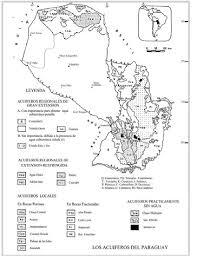
\includegraphics[scale=1]{Imagenes/cap2/images.jpg}
        \caption {Acuíferos del Paraguay} 
        \textbf{Fuente:}
        \cite{alvarez-2014} 
        \label{acuiferosPy}
    \end{figure}




\section{Normativas paraguayas}

La Secretar\'ia del Ambiente (SEAM), a trav\'es de su Direcci\'on General de Protecci\'on y Conservaci\'on de los Recursos H\'idricos (DGPCRH), protege los humedales y gestiona el manejo de los mismos con el fin de su conservaci\'on. Asimismo, la Direcci\'on General de Protecci\'on y Conservaci\'on de la Biodiversidad (DGPCB) es Punto Focal y autoridad de la Ley Nº 350/94 "Que aprueba la Convenci\'on Relativa a los Humedales de Importancia Internacional, especialmente como h\'abitat de aves acu\'aticas”, seg\'un lo establece la Ley Nº 1561/00 que crea el Sistema Nacional del Ambiente,el Consejo Nacional del Ambiente y la Secretar\'ia del Ambiente, en su art/'iculo 14, inciso J.\cite{direccion_general_de_proteccion_y_sitios_nodate}

El Decreto Reglamentario 222/02 establece valores límites para determinados parámetros y representa la referencia de calidad del agua a nivel nacional. Este decreto clasifica el estado de los cuerpos de agua continentales en 4 clases:
\begin{itemize}
    \item Clase 1:
    Aguas destinadas o que puedan ser destinadas al abastecimiento de agua potable a poblaciones con tratamiento convencional.
    \item Clase 2:
    \begin{itemize}
        \item Aguas destinadas al riego de hortalizas o plantas frutícolas u otros cultivos destinados al consumo humano en su forma natural, cuando éstas son usadas a través de sistemas de riego que provocan el mojado del producto.
        \item Aguas destinadas a recreaci\'on por contacto directo con el cuerpo humano.
    \end{itemize}
    \item Clase 3:
    Aguas destinadas a la preservaci\'on de los peces en general y de otros integrantes de la flora y fauna h\'idrica, o tambi\'en aguas destinadas al riego de cultivos cuyo producto no se consume en forma natural o en aquellos casos que siendo consumidos en forma natural se apliquen sistemas de riego que no provocan el mojado del producto.
    \item Clase 4
    Aguas correspondientes a los cursos o tramos de cursos que atraviesan zonas urbanas o suburbanas que deban mantener una armonía con el medio, o también aguas destinadas al riego de cultivos cuyos productos no son destinados al consumo humano en ninguna forma.

\end{itemize}
%%% Tablas 

\begin{table}[htpb]
\caption{L\'imites de par\'ametros f\'isico qu\'imico de aguas. Seg\'un Resoluci\'on 222/02 - SEAM}
\label{tab:Limites222}

\begin{tabular}{lcccc}
\toprule
Par\'ametros                         & Clase I & Clase II & Clase III & Clase IV \\ \noalign{\hrule height 2pt}
                                    &           &            &            &            \\
Oxígeno Disuelto ($mg$ $O_{2}.L^{-1}$) & $\geq$ 6 & $\geq$ 5   & $\geq $4    & $\geq$ 2  \\
                                    &           &            &            &            \\
pH (Unidad de $pH$)                   & 6-9       & 6-9        & 6-9        & 6-9        \\
                                    &           &            &            &            \\
Turbidez ($NTU$)                      & $\leq$ 40 & $\leq$ 100 & $\leq$ 100 & $\leq$ 100 \\
                                    &           &            &            &            \\
Color (real) ($mg$ $Pt.L^{-1}$)       & 15        & 75         & 75         & 75         \\
                                    &           &            &            &            \\
Dureza Total ($mg$ $CaCO_{3}.L^{-1}$) & 750       & 750        & 750        & 750        \\
                                         &           &            &            &            \\
DBO-5 (20º C) ($ mg$ $O_{2}.L^{-1}$)      & 3,0       & 5,0        & 10         &            \\
                                        &           &            &            &            \\
Nitr\'ogeno Total en agua ($mg.L^{-1}$) & 0,3       & 0,6        & 0,6        & 0,6        \\
                                        &           &            &            &            \\
F\'osforo Total en agua ($mg.L^{-1}$)   & 0,025     & 0,05       & 0,05       & 0,05       \\
                                        &           &            &            &            \\
Nitrógeno Amoniacal ($mg.L^{-1}$)       & 0,0165    & 0,0165     & 0,0165     & 0,0165     \\
                                        &           &            &            &            \\
Nitrógeno de Nitritos ($mg/L$)          & 1         & 1          & 1          & 1          \\
                                        &           &            &            &            \\
Nitrógeno de Nitratos ($mg/L$)          & 10        & 10         & 10         & 10         \\
                                    &           &            &            &            \\ 
Cloruro ($mg /L$)                       & 250       & 250        & 250        & 250        \\
                                        &           &            &            &            \\
Sodio ($mg/L$)                          & 200       & 200        & 200        & 200        \\
                                        &           &            &            &            \\
Hierro Ferroso ($mg/L$)                 & 0,3       & 0,3        & 0,3        & 0,3        \\
                                        &           &            &            &            \\
Sulfatos ($mg/L$)                       & 250       & 250        & 250        & 250       \\
\bottomrule
\end{tabular}
\\
\bigskip
\small \textit{Nota}. Extra\'ido de los Art\'iculos 2$^{o}$,3$^{o}$,4$^{o}$,5$^{o}$.\textit{Fuente}. \cite{secretaria-del-ambiente-2022}.
\end{table}

Monitoreo del agua potable: los parámetros químicos comunes incluyen pH, nitratos y oxígeno disuelto. 
La medición de O2 (o DO) es un indicador importante de la calidad del agua. 
Los cambios en los niveles de oxígeno disuelto indican la presencia de microorganismos de aguas residuales, escorrentías urbanas o agrícolas o descargas de fábricas. 
Un nivel adecuado de ORP minimiza la presencia de microorganismos como  E. coli, Salmonella, Listeria . 
Los niveles de turbidez por debajo de 1 NTU indican la pureza adecuada del agua potable.
Detección de fugas químicas en ríos : pH extremo o valores bajos de OD indican derrames químicos debido a problemas en la planta de tratamiento de aguas residuales o en la tubería de suministro.
Medición remota de piscinas : la medición del potencial de oxidación-reducción (ORP), el pH y los niveles de cloro del agua puede determinar si la calidad del agua en piscinas y spas es suficiente para fines recreativos.
Niveles de contaminación en el mar : la medición de los niveles de temperatura, salinidad, pH, oxígeno y nitratos proporciona información para los sistemas de detección de calidad en el agua de mar.
Prevención de la corrosión y depósitos de cal:  Controlando la dureza del agua podemos evitar la corrosión y depósitos de cal en lavavajillas y dispositivos de tratamiento de agua como calentadores. 
La dureza del agua depende de: pH, temperatura, conductividad y concentraciones de calcio (Ca + ) / magnesio (Mg 2+ ).
Cultivo de abetos / Monitoreo de tanques de peces / Criadero / Acuicultura / Acuaponía: Medición de las condiciones del agua de animales acuáticos como caracoles, peces, cangrejos de río, camarones o langostinos en tanques. 
Los valores importantes son el pH, el oxígeno disuelto (DO), el amoníaco (NH 4 ), el nitrato (NO 3 - ), el nitrito (NO 2 - ) y la temperatura del agua.
Hidroponía : las plantas que toman los nutrientes directamente del agua necesitan un pH preciso y niveles de oxígeno en el agua (OD) para obtener el máximo crecimiento.

Las sondas del sensor miden más de 12 parámetros químicos y físicos de la calidad del agua, como pH, nitratos (NO3), iones disueltos (fluoruro (F - ), calcio (Ca 2+ ), nitrato (NO 3 - ), cloruro (Cl - ), Yoduro (I - ), Cúprico (Cu 2+ ), Bromuro (Br - ), Plata (Ag + ), Fluoroborato (BF 4 - ), Amoníaco (NH 4 ), Litio (Li + ), Magnesio (Mg 2+ ) , Nitrito (NO 2- ), Perclorato (ClO 4 ), Potasio (K + ), Sodio (Na +) oxígeno disuelto (OD), conductividad (salinidad), potencial de oxidación-reducción (ORP), turbidez, temperatura, etc. Los contaminantes pueden detectarse y tratarse en tiempo real para garantizar una buena calidad del agua en toda la red de suministro de agua. Los valores extremos de pH pueden indicar derrames de productos químicos, problemas en la planta de tratamiento o problemas en las tuberías de suministro. Los niveles bajos de OD pueden indicar la presencia de microorganismos debido a escorrentías urbanas / agrícolas o derrames de aguas residuales. El ORP mide qué tan bien está funcionando la desinfección del agua.

\section{Calidad del agua.}
%Tema pendiente de ver 
%Preguntar en http://habitat.aq.upm.es/dubai/00/bp561.html sobre los parametros y estandares Py.
%%%%%%%%%

El término calidad del agua se utiliza para describir el estado del agua, incluida su características químicas, físicas y biológicas, generalmente con respecto a su idoneidad para un propósito particular (es decir, beber, nadar o pescar)~\cite{waterquality}.

La calidad del agua se puede considerar como una medida de la idoneidad del agua para un uso particular en función de determinadas características físicas, químicas y biológicas. 
Para determinar la calidad del agua, los técnicos primero miden y analizan las características del agua, como la temperatura, el contenido de minerales disueltos y la cantidad de bacterias. 
Luego, las características seleccionadas se comparan con normas y pautas numéricas para decidir si el agua es adecuada para un uso particular. 
La calidad es el estado de las características físicas, biológicas y químicas del agua basados en condiciones establecidas

Los parámetros óptimos de las características físicas, químicas y biologías del agua, se establecen según las normas de los organismos reguladores. 
En Paraguay el organismo regulador 
% [RR] Concluir esta sección con los parámetros de algún organismo 

\section{Sensores para calidad de agua.}

Las características químicas, físicas y biológicas del agua se combinan para formar lo que denominaremos calidad del agua. 
Mínimos cambios en estas características pueden poner en peligro los ecosistemas. 
Para preservar su calidad, la monitorización precisa de los parámetros del agua como la conductividad, el pH, la salinidad, la temperatura, el oxígeno disuelto (OD), OPR, son fundamentales. 
A continuaci\'on  describiremos los sensores de calidad del agua que son adecuados tanto para puntos simples requisitos de muestreo y proyectos complejo.

Existen varios parámetros que pueden estudiarse para indicar la calidad del agua.
Estos parámetros pueden medirse ya sea de características físicas como el pH, conductividad, o temperatura; niveles de varios nutrientes en agua, como nitratos y fosfatos; o de algunos elementos y compuestos del agua, como el oxígeno disuelto. 

Existen una gran variedad de sensores para la obtención de las mediciones de los índices de calidad del agua, en el presente TFG abordaremos los sensores de pH, conductividad eléctrica, oxigeno disuelto, potencial de oxido reducción y temperatura. 

\subsection{Medición de pH}
\subsubsection{¿Qué es pH?}

El valor de pH describe la actividad de los iones de hidrógeno en soluciones. 
Por análisis químicos se sabe que el pH siempre se encuentra en una escala de 0 a 14. 
Es importante decir que el pH mide el grado de acidez o de alcalinidad pero no determina el valor de la acidez ni de la alcalinidad \cite{sierra_ramirez_calidad_2011}. 
Con base en esta escala de pH, los líquidos se caracterizan por ser ácidos, alcalinos o neutros; una solución que no es ácida ni alcalino es neutro, lo que corresponde a un valor de 7 en la escala de pH. 
La acidez indica una mayor actividad de los iones de hidrógeno y un valor de medición de pH inferior a 7. 
Las soluciones alcalinas se caracterizan por un ion de hidrógeno más bajo actividad o mayor actividad de iones de hidróxido, respectivamente, y una medición de pH valor por encima de 7.
La escala de pH es logarítmica. Una diferencia de una unidad de medida de pH representa un aumento o reducción de 10 veces, o 10 veces, de la actividad de los iones de hidrógeno en la solución~\cite{covington_definition_1985}.

\begin{equation} \label{ecuacionpH} 
%%\[pH= -\log_{10}[H^{+}\]
pH=-log_{10}[H^{+}]
\end{equation}


\subsubsection{¿Como medirlo?}
Existen varias formas de medir esta magnitud química, se puede medir utilizando sistemas de medición electroquímicos, papel tornasol o indicadores, electrodos, amperímetros, ISFET entre otros. 

\begin{itemize}
    \item Papel tornasol: La forma más sencilla de medir el pH es usar los indicadores o tiras de tornasol, son simples y económicos. 
    Desafortunadamente, en muchos casos el papel tornasol y indicadores no son lo suficientemente precisos para realizar mediciones de pH de alta calidad. 
    Ambos métodos proporcionan un pH basado en una reacción química que hace que cambie el color. 
    Si la muestra de papel o líquido cambia de color, se debe comparar con la escala de colores y allí, según el usuario, elegir el que mejor se adapte.
    
    \begin{figure}[H]
        \centering
        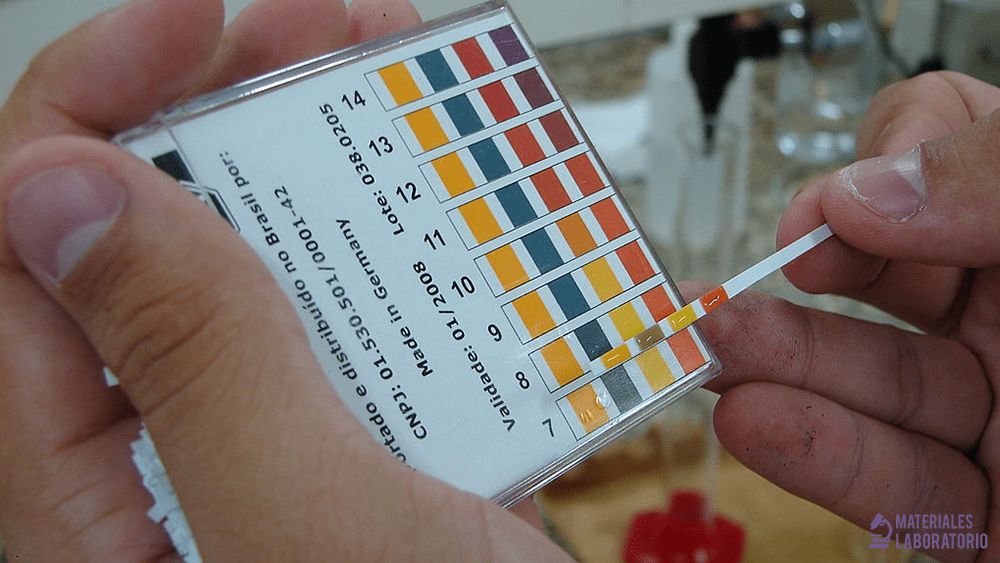
\includegraphics[width=100mm, height=65mm]{Imagenes/cap2/Papel-tornasol-min.png}
        \caption {Papel tornasol o papel pH. \textbf{Fuente:} \cite{noauthor_papel-tornasol-min-768x432png_nodate} }
        \label{fig:tornasol}
    \end{figure}
    
    \item Amperometría: La diferencia en la concentración de iones de hidrógeno (fuera de la sonda vs. dentro de la sonda) crea una corriente muy pequeña. 
    Esta corriente es proporcional a la concentraci\'on de iones de hidrógeno en el líquido medido \cite{Atlas_pH}. 
    La ventaja de la amperometría como método de medición del pH es que es fácil de usar. 
    En mediciones amperométricas de pH generación de hidrógeno ocurre en un metal noble, cuando se combina con un metal menos noble, se forma una c\'elula galvánica de distribución de energía. 
    Debido a que se generan iones de hidrógeno, la corriente de la c\'elula depende del valor del pH. 
    Las desventajas de este método son que las diferencias en la composición de la muestra crean errores muy grandes en las mediciones de pH y el método no puede ofrecer resultados fiables en ácidos y bases extremadamente concentrados, debido a efectos relacionados con la membrana de cristal. 
    
    \begin{figure}[H]
        \centering
        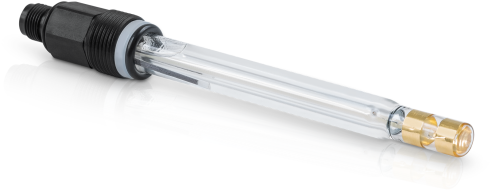
\includegraphics[width=100mm, height=65mm]{Imagenes/cap2/amperimetrico.png}
        \caption {Sensor OPTISENS CL 1100.} \textbf{Fuente:}
        \cite{ampe_sensores_nodate} 
        \label{fig:amperimetrica}
    \end{figure}
    
    \item ISFET: \textit{Ion Sensitive Field Effect Transitor} o transistor de efecto campo sensible a iones en un sensor electroqu\'imico que reaccionan a cambios en la actividad de un ion dado, un m\'etodo relativamente nuevo para la medici\'on del valor de pH \cite{duroux_ion_1991}.
    
    Es un transistor con fuente de poder y desagüe, dividido por un aislador. 
    Este aislador (puerta) está hecho de un óxido metálico donde los iones de hidrógeno se acumulan de la misma manera que un electrodo. 
    La carga positiva que se acumula fuera de la puerta se ``refleja'' en el interior la puerta por una carga negativa igual generada. 
    Una vez que esto sucede, la puerta comienza a conducir electricidad. 
    Cuanto menor sea el valor de pH, más iones de hidrógeno se acumulan y más corriente puede fluir entre la fuente y el drenaje. 
    El ISFET Los sensores, similares a los electrodos de pH de vidrio, actúan de acuerdo con la ecuación de Nernst.
    La ventaja de un ISFET es que es muy pequeño. 
    El transistor de efecto de campo real (FET) es de solo \(0.2 mm^{^{2}}\). 
    La desventaja de usar un ISFET para mediciones de pH es que tienen una durabilidad comparativamente corta y una baja duración a largo plazo~\cite{li_chapter_2019}.
    
    \begin{figure}[H]
        \centering
        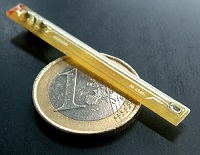
\includegraphics[width=70mm, height=45mm]{Imagenes/cap2/ISFET_Euro.jpg}
        \caption {Sensor de pH-ISFET MSFET 3330. \textbf{Fuente:}
        \cite{microsens_nodate} }
        \label{fig:isfet}
    \end{figure}
    
    \item Electrodos: El método más común de medición del valor de pH es el uso de electrodos.
    Estos dispositivos de medición de pH son sensores electroquímicos que constan de un electrodo de medición y un electrodo de referencia. 
    El electrodo de medición de pH está hecho de vidrio especial que, debido a sus propiedades superficiales, es particularmente sensible a iones de hidrógeno. 
    El electrodo de medición de pH se llena con una solución tampón de un valor de pH de 7. 
    Al colocar el electrodo de medición de pH en una prueba soluci\'on, el cambio de voltaje se mide con el electrodo de pH comparando el voltaje medido al electrodo de referencia estable. 
    Este cambio se registra por el medidor de pH y se convierte en el valor de medición de pH que se muestra.
    
    \begin{figure}[H]
        \centering
        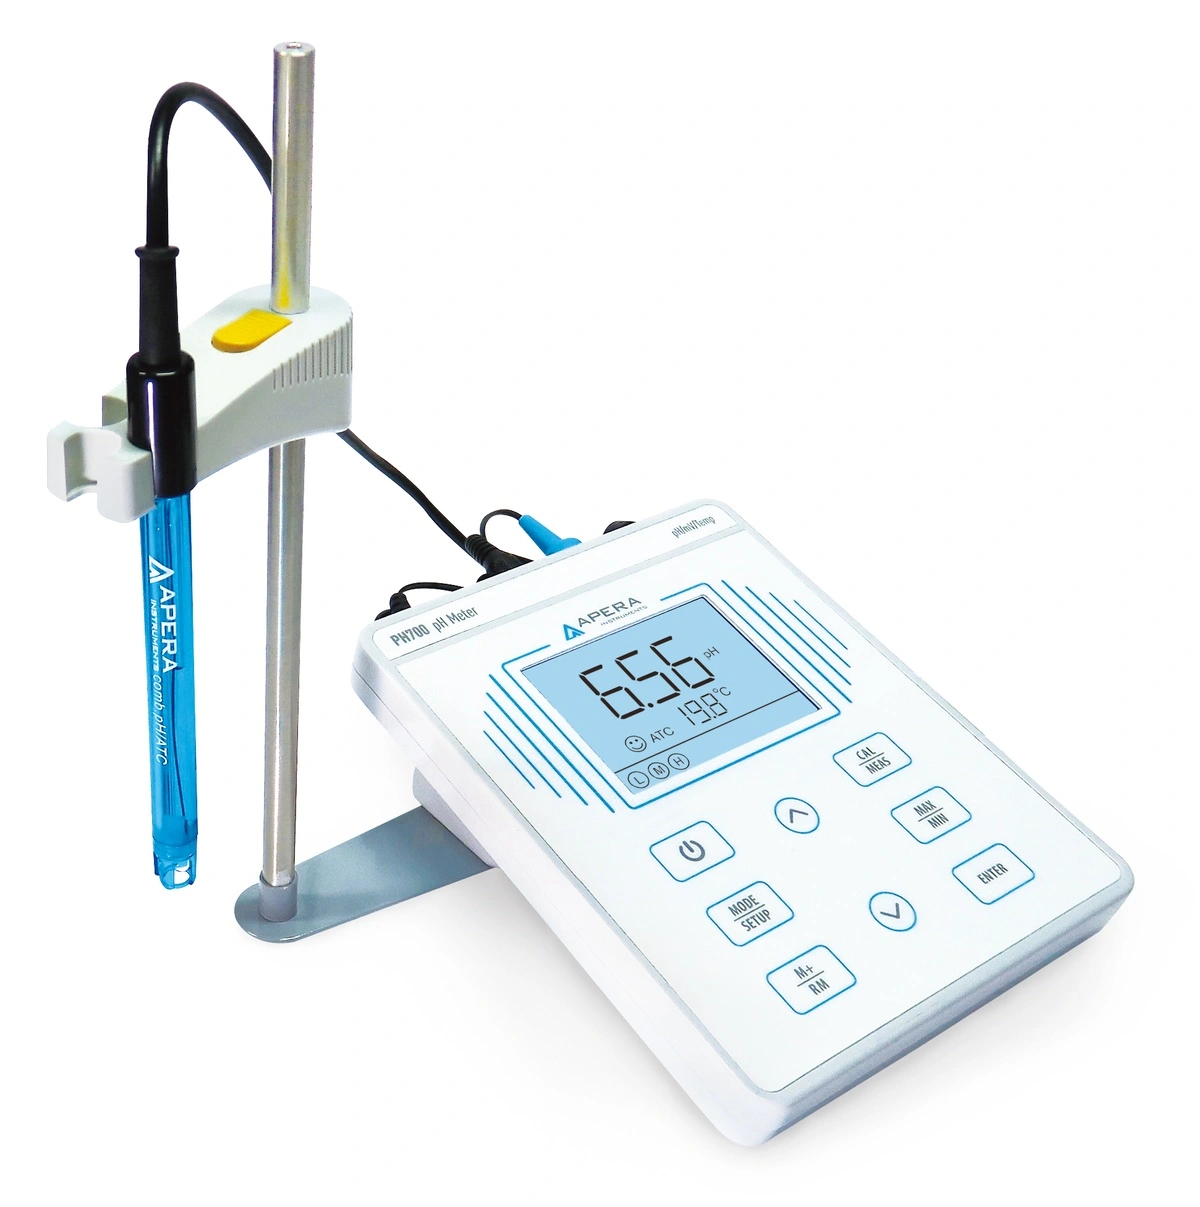
\includegraphics[width=60mm, height=45mm]{Imagenes/cap2/ph700.png}
        \caption {PH700 Benchtop pH Meter Kit. \textbf{Fuente:}
        \cite{ph700_nodate} }
        \label{fig:ph700}
        \end{figure}
\end{itemize}

    De todos estos métodos de medición del valor de pH,  el mejor es el uso de electrodos de pH. 
    No hay otro sistema de medición de pH que proporcione mejor confiabilidad, precisión y velocidad de la medición del pH en todo el pH distancia. 
    La desventaja mínima de usar electrodos de vidrio para pH para este método de medición de pH es el hecho de que los electrodos de vidrio son delicados y deben manipularse con cuidado~\cite{li_chapter_2019}.

\subsubsection{Sensor de potencial de hidrógeno (pH)}

El medidor de pH es un instrumento utilizado para medir la acidez o la alcalinidad de una solución, también llamado de pH. El pH es la unidad de medida que describe el grado de acidez o alcalinidad y es medido en una escala que va de 0 a 14, con 0 siendo una solución de ácido fuerte y 14 una solución básica fuerte.
Es una manera de evaluar que tan adecuada es el agua para una planta o animal.  Si el agua es demasiado ácida o básica, ya sea a por contaminantes naturales o de origen humano, puede ver un impacto profundamente negativo a la vida acuática.  Un pH normal en cuerpos de agua tiene un valor de entre 5.0 a 9.0, pero de manera ideal debería estar en un rango de entre 6.0 a 8.0. %poner refdel 2222

\subsubsection{¿Cómo medir el pH?}
Test de pH comunes cómo los test kit químicos y tiras de tornasol, son simples y económicos. 
Aun así, estos métodos tienen inconvenientes que pueden causar resultados imprecisos. 
Ambos métodos entregan un valor de pH basado en una reacción química que resulta en el cambio de color. 
Cuando su papel o muestra líquida cambia de color, debe compararlo con la guía de color y allí seleccionar la que más se ajuste según su criterio.
Las informaciones cuantitativas dadas por el valor del pH expresan el grado de acidez de un ácido o de una base en términos de la actividad de los iones de hidrógeno. 
El valor del pH de determinada sustancia está directamente relacionado a la proporción de las concentraciones de los iones de hidrógeno [H+] e hidroxilo [OH-]. 
Si la concentración de H+ es mayor que la de OH-, el material es ácido; el valor del pH es menor que 7. 
Si la concentración de OH- es mayor que la de H+, el material es básico, con un pH con valor mayor que 7. 
Si las cantidades de H+ y de OH- son las mismas, el material es neutral y su pH es 7. Ácidos y bases tienen, respectivamente, iones de hidrógeno y de hidroxilo libres. 
La relación entre los iones de hidrógeno y de hidroxilo en determinada solución es constante para un dado conjunto de condiciones y cada uno puede ser determinado desde que se conozca el valor del otro.
Una lectura más precisa significa que es necesario utilizar un medidor de pH. 
Cuando está eligiendo un tester o medidor de pH, existen múltiples consideraciones relacionadas tanto al electrodo como al dispositivo que deben tenerse en cuenta. 
Asegúrese de encontrar un medidor de pH y un electrodo que mejor se ajuste a su área de trabajo.


El medidor de pH es un instrumento utilizado para medir la acidez o la alcalinidad de una solución, también llamado de pH. El pH es la unidad de medida que describe el grado de acidez o alcalinidad y es medido en una escala que va de 0 a 14, con 0 siendo una solución de ácido fuerte y 14 una solución básica fuerte.

Las informaciones cuantitativas dadas por el valor del pH expresan el grado de acidez de un ácido o de una base en términos de la actividad de los iones de hidrógeno. El valor del pH de determinada sustancia está directamente relacionado a la proporción de las concentraciones de los iones de hidrógeno [H+] e hidroxilo [OH-]. Si la concentración de H+ es mayor que la de OH-, el material es ácido; el valor del pH es menor que 7. Si la concentración de OH- es mayor que la de H+, el material es básico, con un pH con valor mayor que 7. Si las cantidades de H+ y de OH- son las mismas, el material es neutral y su pH es 7. Ácidos y bases tienen, respectivamente, iones de hidrógeno y de hidroxilo libres. La relación entre los iones de hidrógeno y de hidroxilo en determinada solución es constante para un dado conjunto de condiciones y cada uno puede ser determinado desde que se conozca el valor del otro.


\subsection{Medición de potencial ORP-REDOX}
\subsubsection{¿Que es ORP?}
El potencial de oxidacion-reduccion (ORP) se define como la fuerza electromotriz entre un electrodo de metal noble y un electrodo de referencia cuando se sumergen en una solución.
Los electrodos de ORP son inertes y miden la relación entre las actividades de las especies oxidadas y las reducidas presentes~\cite{d19_committee_test_nodate}.
También conocido como redox, es una medida en milivoltios y mide el potencial de intercambio de electrones, si una sustancia (generalmente liquida) se oxida o se reduce. 
Los oxidantes siempre tendrán un valor de ORP positivo, mientras que los reductores siempre tendrán un valor de ORP negativo. 
El ORP se usa comúnmente para medir la limpieza en los sistemas de agua y la descomposición de productos de desecho, escombros y contaminantes. 
La composición química del agua subterránea y los sistemas de acuíferos contaminados se ven afectados por procesos de reducción de oxidación (redox)~\cite{wator_redox_2020}.

\subsubsection{¿Cómo medirlo?}
Un sensor de ORP consta de un electrodo de ORP y un electrodo de referencia.
Los electrodos de ORP miden de forma fiable el ORP en casi todas las soluciones acuosas y, en general, no están sujetos a la interferencia de la solución por el color, la turbidez, la materia coloidal y la materia en suspensión~\cite{d19_committee_test_nodate}.

El electrodo OPR: el principio detras de la medicion de ORP es el uso de un electrodo de metal inerte (platino, a veces oro), que, debido a su baja resistencia, cedera electrones a un oxidante o aceptara electrones de un reductor. 
El electrodo de ORP continuará aceptando o cediendo electrones hasta que desarrolle un potencial, debido a la carga acumulada, que es igual al ORP de la solución. 
La precisión típica de una medida de ORP es d\'e \( \pm5 mV\).

El electrodo de referencia:  ser el mismo electrodo de plata-cloruro de plata utilizado con mediciones de pH~\cite{li_chapter_2019}.

    \begin{figure}[H]
        \centering
        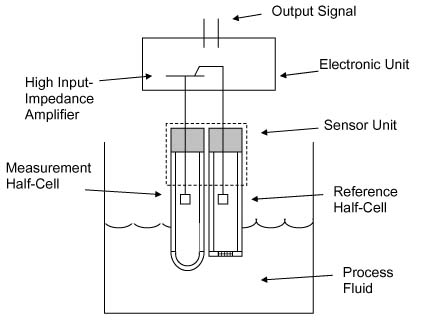
\includegraphics[width=80mm, height=80mm]{Imagenes/cap2/ORP_Sensor_Image.jpg}
        \caption {Diagrama del sensor OPR. \textbf{Fuente:}
        \cite{orp_sensor_measure_nodate} }
        \label{fig:opr}
    \end{figure}


\subsubsection{Sensor de potencial de \'oxido reducción (OPR)}
Los sensores de potencial de reducción de la oxidación (ORP) miden la habilidad de una solución de actuar como agente oxidante o reductor. 
Para conseguir resultados exactos, es importante contar con una combinación correcta de sistema de referencia, unión y forma. METTLER TOLEDO ofrece sensores de ORP (Redox) con superficies de metal lisas y uniones de referencias únicas para garantizar unas mediciones fiables, incluso con muestras sucias.

\subsection{Temperatura}
\subsubsection{¿Qué es temperatura?}
La temperatura es una de las medidas más comunes en la vida diaria. 
En el contexto de calidad de agua, la temperatura puede proveer un indicio de las condiciones de vida para plantas acuáticas y animales.  
Las temperaturas templadas se consideran generalmente benéficas para el crecimiento de la población acuática. 
De cualquier forma, después de cierto punto la temperatura puede tener un efecto contrario, contribuyendo a declinar la diversidad biológica en cuerpos de agua.

\subsubsection{¿Porque la medición de temperatura es importante?}
Organismos acuáticos cómo los peces y plancton son de agua fría, así que la temperatura en el agua tiene un impacto directo en la temperatura de su cuerpo. 
Estos organismos tienen rangos de temperatura en los cuales pueden sobrevivir y desarrollarse. 
A medida que la temperatura alcanza el límite superior o su rango para un organismo, la actividad biológica estará en su tope. 
La actividad disminuirá cuando se alcance el punto mínimo del rango. 
Si la temperatura excede el rango aceptable para el organismo, la cantidad disponible de oxígeno puede ser demasiado baja para sustentarlos. 
Esto se debe a que el agua caliente tiene un punto de saturación de ox\'igeno menor al agua fría. 
Si la temperatura está por debajo del rango aceptable, no hay suficiente actividad para el crecimiento de los organismos. 
La temperatura alta también contribuye al crecimiento y floración de algas. 
El oxígeno se consume en la medida que bacterias descompongan estos brotes, lo que reduce la cantidad de oxígeno disuelto disponible.
La temperatura en varios cuerpos de agua se basa en la hora del día y la cantidad de luz solar calentando la superficie. 
Las temperaturas aceptables también varían dependiendo del tipo de río o corriente de agua que desee monitorear. 
Esto depende de la fuente de la cuenca que alimenta la corriente. 
Si se alimenta la corriente con agua de manantial, por ejemplo, la temperatura normal de la corriente puede ser adecuada (menor a 68 68$^\circ$ F). 
Una corriente se considera templada si tiene una temperatura promedio superior a los 68$^\circ$ F, pero menor a los 89$^\circ$ F. 
La temperatura también puede verse influenciada por el flujo y el cuerpo de agua. 
Si el flujo de agua se incrementa, quizá cómo resultado de una fuerte lluvia, se puede esperar que la temperatura disminuya. 
El incremento en la corriente tiene cómo efecto reducir la temperatura en el agua.

La polución por temperatura, también conocida cómo polución térmica, puede ser causada por vertimientos de agua calentada en asfalto o concreto. 
Esta también puede proceder de efluentes industriales que sean descargados en cuerpos de agua, o agua que sea usada cómo refrigerante en plantas de energía nuclear. 
Estos efluentes significan que el agua en el que son descargadas incrementará la temperatura general del cuerpo de agua.  
La temperatura también puede asociarse a la turbidez.  
Ya que la cantidad de luz absorbida incrementa a medida que el agua se oscurece, la temperatura también aumentará.

\subsubsection{¿Cómo medir la temperatura?}
Muchos termómetros simples usan un termistor.  
El termistor es un dispositivo semiconductor cuya resistencia varía en función de la temperatura.  
A medida que la temperatura incrementa, la resistencia disminuye.  
La resistencia medida por el termistor se convierte en un valor que se muestra ya sea en la escala Celsius o Fahrenheit.  
Los sensores termistores son adecuados para rangos de temperatura desde -50° a 150°C (-58° a 302°F).

\subsubsection{Calibración de temperatura}
Muchos medidores se calibran en fábrica para las lecturas de temperatura. 
Es una buena práctica revisar esta calibración al menos una vez al año en un laboratorio, y asegurar que el sensor de temperatura funciona de manera adecuada.

\subsubsection{Sensor de temperatura (T)}
La temperatura se puede medir utilizando un sensor de temperatura de los diferentes tipos que existen. 
Todos ellos infieren la temperatura al detectar algún cambio en una característica física. 
Hay seis tipos de sensor de temperatura con los cuales es probable que el ingeniero se encuentre: termopares, dispositivos de temperatura resistivos (RTD y termistores), radiadores infrarrojos, dispositivos bimetálicos, dispositivos de dilatación de l\'iquido, y dispositivos de cambio de estado.
Un termopar es un sensor para medir la temperatura. 
Se compone de dos metales diferentes, unidos en un extremo. Cuando la unión de los dos metales se calienta o enfría, se produce una tensión que es proporcional a la temperatura. 
Las aleaciones de termopar están comúnmente disponibles como alambre.
Los termopares están disponibles en diferentes combinaciones de metales o calibraciones para adaptarse a diferentes aplicaciones. 
Los tres más comunes son las calibraciones tipo J, K y T, de los cuales el termopar tipo K es el más popular debido a su amplio rango de temperaturas y bajo costo.

\subsection{Conductividad (CE) / Total de sólidos disueltos (TDS)}

\subsubsection{¿Qué es la conductividad?}
La conductividad eléctrica (CE) mide que tan bien una sustancia puede transmitir una corriente eléctrica. 
Pequeñas partículas cargadas, llamadas iones, pueden ayudar a transportar la corriente eléctrica a través de la substancia. 
Estos iones pueden estar cargados positiva, o negativamente. A mayor cantidad de iones disponibles, mayor será la conductividad; menores iones resultarán en una menor conductividad. 
La CE se reporta de manera habitual en milliSimens por centímetro (mS/cm).

El total de sólidos disueltos (TDS) es la cantidad de sustancias disueltas en soluciones. 
Las mediciones permiten conocer las sustancias orgánicas e inorgánicas disueltas en el líquido. 
Los resultados de esta lectura se muestran en miligramos por litro (mg/L), partes por mill\'on (ppm), gramos por litro (g/L), o partes por mil (ppt).

\subsubsection{¿Por qu\'e la medici\'on de conductividad es importante?}
La conductividad eléctrica (CE) es otra manera de evaluar la calidad del agua, ya que al incrementar la presencia de total de sólidos disueltos (TDS), expresada en la CE, puede ser un indicador de contaminantes. 
La CE puede verse afectada por los carbonatos presentes en el agua caliza, contaminantes humanos como aguas residuales u otro tipo de fuente cómo sistemas de pozos sépticos o residuos de agricultura.

Altas concentraciones de TDS pueden reducir la calidad de agua y causar problemas en el balance de agua para organismos individuales. 
Por otra parte, bajas concentraciones pueden limitar el crecimiento de vida acuática. 
Algunos de los efectos comentados para parámetros como el dióxido de carbono y acidez tienen relevancia para la CE, cómo su impacto negativo en la fotosíntesis. 
Esto se debe a que al incrementar la cantidad de sólidos el agua se oscurecerá, reduciendo la tasa de fotosíntesis. 
La CE proveerá un indicio del total de sólidos disueltos, del cual el total de sales disueltas es un componente. 
Si el nivel de sales en el TDS es alto, esto también puede contribuir a acidificar el agua. 
De cualquier forma, si el nivel de carbonatos en la lectura de TDS son altos, esto podría contribuir a incrementar la alcalinidad, lo que puede ayudar a proteger el agua ante cambios ácidos. 
Esta es una buena respuesta de interrelación, entre los parámetros de calidad de agua.

Niveles aceptables de CE en ríos y corrientes de agua varía dependiendo del tipo de sólidos disueltos presentes y esto determina el uso de la corriente, ya sea para pesca, nado o como una fuente de agua potable.


Corriente
Es importante comprender la relación entre TDS y sólidos totales. Los sólidos totales se refieren a toda la materia sólida, ya sea suspendida o disuelta en agua. 
Los sólidos disueltos no son visibles en el agua, ya que al disolverse se vuelven parte de la solución. 
Los TDS son una medida de las sustancias disueltas en agua que están en una muestra de agua. 
En una muestra recolectada en un rio, estas sustancias disueltas se conocen cómo solutos, y el agua es llamada solvente.

\subsubsection{¿Cómo medir la conductividad?}
La mejor manera de medir la conductividad es con el uso de un medidor. 
Dos electrodos que aplican un voltaje AC se ubican en la solución. 
Esto crea una corriente que depende de la conductividad natural de la solución. 
El medidor lee esta corriente y muestra la conductividad (CE) o ppm (TDS)

\subsubsection{Calibración de conductividad en campo}
Es importante calibrar la conductividad antes de analizar la muestra. 
Esto se debe a que recubrimientos aceitosos y contaminantes biológicos puede cambiar la geometría celular, resultando en una desviación en la constante celular. 
Antes de realizar la calibración de conductividad, siempre inspeccione el sensor de CE por residuos u obstrucciones.

La mayoría de los medidores se calibran con un solo estándar, procurando que este cerca de la conductividad de la muestra a medir. 
Un segundo estándar puede usarse para revisar la linealidad del instrumento en el rango de medición.

\subsubsection{Procedimiento de calibración}:
Llene el beaker con suficiente estándar para cubrir la unión del electrodo (cerca de 75 mL de un beaker de 100 mL) 
Vierta solución adicional en un segundo beaker para enjuagar el sensor.
Ubique el electrodo en el beaker de enjuague y asegúrese de que los canales del sensor de CE estén llenos con estándar fresco al enjuagar y agitar la sonda en el beaker unas cuantas veces.
Ubique la sonda en el beaker de calibración y golpee suavemente para liberar burbujas atrapadas.
Confirme el punto de calibración cuando la lectura sea estable, o cuando los dígitos no cambien por al menos 5 segundos. (Algunos medidores requerirán que ingrese el valor del estándar de conductividad)
La calibración esta completa. Enjuague la sonda con agua desionizada y almacénela de acuerdo a las instrucciones del fabricante.


\subsubsection{Sensor de conductividad eléctrica (CE) }
La salinidad de un suelo o agua, se refiere a la cantidad de sales presentes en solución, y puede ser estimada indirectamente mediante la medición de la conductividad eléctrica (CE). 
El valor de CE es influenciado por la concentración y composición de las sales disueltas. 
A mayor valor de CE, mayor es la salinidad presente. 
Es importante considerar que todos los fertilizantes inorgánicos son sales y por lo mismo tienen un efecto directo sobre la CE.

La salinidad es un fenómeno indeseable ya que afecta el crecimiento de las plantas  de varias maneras y por lo mismo, un aumento en la CE traerá como consecuencia una disminución de rendimiento.

\subsection{Oxígeno disuelto (OD)}
\subsubsection{¿Qué es el oxígeno disuelto?}
La concentración de oxígeno disuelto (OD) en agua es extremadamente importante en la naturaleza, al igual que para los ambientes artificiales.  
En océanos, lagos, ríos, y otros grandes cuerpos de agua, el oxígeno disuelto es esencial para el crecimiento y desarrollo de la vida acuática.  
Sin oxígeno, el agua puede volverse tóxica debido al decaimiento de la materia orgánica por bacterias anaeróbicas. 
En un ambiente industrial, el agua debe contener al menos 2 mg/L de oxígeno para proteger a las tuberías de corrosión.  
De cualquier manera, los sistemas de agua de calderas, en muchos casos no pueden contener más que 10 mg/L de oxígeno disuelto.

\subsubsection{¿Porque es importante el oxígeno disuelto?}
Los niveles de OD pueden ayudar a indicar la salud de un cuerpo de agua. 
Si los niveles de OD están dentro de la media o más altos, el agua es un buen ambiente para una amplia variedad de vida acuática. 
Si los niveles de OD son bajos, indica la presencia de contaminantes en el agua. 
Algunas especies de vida acuática pueden subsistir en agua con un amplio rango de OD; pero otras fallecen a bajos niveles de OD.

Oxígeno disuelto
Se espera que las lecturas de OD tengan una amplia fluctuación si la fuente de agua cuenta con abundante vida vegetal. 
Esto se debe al proceso de fotosíntesis. 
Ya que existe una menor actividad fotosintética en las noches, cuando la luz no está presente, y que tanto plantas como animales seguirán consumiendo oxígeno a través de la respiración, los niveles de OD en las horas de la mañana serán mucho menores a los de otras horas del día. 
Una vez inicia la fotosíntesis, los niveles de OD incrementarán. 
Este es un buen ejemplo de los beneficios de medir los parámetros varias veces durante el día. 
Si únicamente se realiza la medición de OD antes del amanecer, se llegará a una conclusión inadecuada sin importar la salud del cuerpo de agua.

Mientras que los niveles de OD se influencian particularmente por la actividad fotosintética, una gran cantidad de OD se obtiene de la mezcla del OD y el agua. 
Esto sucede si el agua es turbulenta en grandes cuerpos de agua. 
La turbulencia incrementa el área superficial del agua, para que el oxígeno atmosférico puede mezclarse más fácilmente. 
El aire tiene una concentración de oxígeno que es 20 veces mayor que la concentración de oxígeno en el agua. 
La diferencia de concentración resulta en el oxígeno atmosférico disolviéndose en agua cuando las dos se encuentran. 
Si hay más superficie de agua en su interfaz, entonces más oxígeno del aire se absorberá.

Otros factores que influencian los niveles de OD son la temperatura y los vertimientos. 
El oxígeno se disuelve más fácilmente en agua fría, y el agua fría tiene la capacidad de mantener mayores cantidades de gas que el agua tibia, así que el nivel de OD disuelto disminuye a medida que el agua se calienta. 
Los vertimientos pueden incluir desechos orgánicos o contaminantes creados por el hombre; en ambos casos, los organismos en el agua deben usar oxígeno en el proceso de descomponer estos contaminantes.  
También, los desechos orgánicos pueden llevar al crecimiento de vegetación acuática.  
Cuando las plantas mueren al final del lapso de crecimiento, grandes cantidades de oxígeno disuelto se consumen al descomponerse.

\subsubsection{¿Cómo podemos medir el oxígeno disuelto?}
Las concentración de oxígeno disuelto se reporta en miligramos de gas por litro de agua, mg/L. (La unidad equivalente a mg/L es equivalente a partes por millón=ppm)  

Las lecturas de OD se realizan habitualmente utilizando una sonda y un medidor.

 
Es importante realizar lecturas de OD en varios momentos del día, y a varias profundidades. 
Las mediciones le darán una visión general de los niveles de OD en el cuerpo de agua que investiga. 
Cómo sucede con todos los parámetros de calidad de agua, este parámetro debe monitorearse en el tiempo. 
Esto producirá suficiente información para identificar y evaluar tendencias.

\subsubsection{Calibración de OD en campo}
El contenido de oxígeno disuelto (OD) en el agua se mide usando un electrodo con membrana. 
Desafortunadamente, cepillos u otros objetos de limpieza pueden dañar la membrana, así que remplazar la tapa de la membrana y el electrolito es la mejor manera de realizar un mantenimiento periódico. 
Si bien es más fácil calibrar el sensor de OD antes de estar en campo, es mejor calibrar la sonda en campo pues las diferencias de altitud y presión barométrica entre la calibración y la lectura pueden resultar en errores. 
Asegúrese de verificar que las lecturas de presión barométrica, conductividad, y temperatura sean correctas.

\subsubsection{Procedimiento de calibración (100\%)}:

Llene un beaker de calibración con agua (como alternativa ubique una esponja húmeda o una toalla de papel húmeda en el fondo del contenedor usado para la calibración)
Ajuste ligeramente la sonda en el beaker de calibración para evitar escape de humedad. 
Asegúrese de no humedecer su sensor de OD por la evaporación en el sensor de temperatura pues esto puede influenciar las lecturas de la sonda durante la calibración.
Permita al contenedor saturarse con vapor de agua (por aproximadamente 10 a 15 minutos). 
Durante este periodo, encienda el instrumento para permitir que la sonda de O.D. caliente
Confirme el punto de calibración cuando la lectura sea estable, o cuando los dígitos no cambien por al menos 5 segundos.
La calibración esta completa. 
Enjuague la sonda con agua desionizada y almacénela de acuerdo a las instrucciones del fabricante.

\subsubsection{Procedimiento de calibración (0\%):}
Llene el beaker con suficiente solución 0\% OD para cubrir la unión del electrodo (cerca de 75 mL de un beaker de 100 mL)
Sumerja la sonda de OD en la solución.
Confirme el punto de calibración cuando la lectura sea estable, o cuando los dígitos no cambien por al menos 5 segundos.
La calibración esta completa. 
Enjuague la sonda con agua desionizada y almacénela de acuerdo a las instrucciones del fabricante. 
Asegúrese de enjuagar toda la solución $0\%$ OD para que esta no afecte las mediciones de sus muestras.

\subsubsection{Sensor de oxigeno disuelto (DO):}
Toda la vida acuática depende de la disponibilidad de oxígeno disuelto (DO) en el agua. 
Mientras que los organismos terrestres viven en una atmósfera compuesta aproximadamente de un 20\% de oxigeno, los organismos acuáticos sobreviven con una cantidad de oxigeno considerablemente menor. 
La solubilidad del oxigeno en agua dulce varia entre 14.6 mg/L a 0$^{\circ}$C hasta aproximadamente 7 mg/L a 35$^{\circ}$C bajo una presión de 760 mmHg. La concentración de oxígeno disuelto en agua está determinada por la ley de Henry, que describe la relación de equilibrio entre la presión parcial de oxígeno atmosférico y la concentración de oxígeno en agua. 
Otros factores que influyen la concentración de oxígeno disuelto en agua son: la presión atmosférica (y por lo tanto la altitud sobre el nivel del mar), el contenido de sales en el agua, y la temperatura del agua. 
El contenido de oxigeno disuelto en cuerpos de agua puede disminuir significativamente por efecto de la respiración, especialmente la microbiana, resultante de la degradación de compuestos orgánicos. 

Traducido eso a un sensor cual permita detectar estos factores, se tiene la sonda galvánica de oxigeno disuelto que consta de una membrana de politetrafluoroetileno (PTFE), un ánodo bañado en un electrolito y un cátodo. 
Las mol\'eculas de oxígeno se desactivan a través de la membrana de la sonda a una velocidad constante (sin la membrana, la reacción es rápida). 
Una vez el las mol\'eculas de oxigeno han atravesado la membrana se reducen en el cátodo y se produce una pequeña tensión. 
Si no hay moléculas de oxígeno presentes, la sonda emitiría 0 mV. 
A medida que aumenta el ox\'igeno, tambi\'en lo hace la salida de mV de la sonda. La sonda emite un voltaje diferente en presencia de ox\'igeno. Lo \'unico que es constante es que 0mV = 0 ox\'igeno []

emitite

%%%%%%%%%%%%%%%%%%%%%%%%%%%%%%%%%%%%%%%%%%%%%%%%%%%%%%%%%%%%%%%%%%%%%%%%%%%%%%%%%%%%%%%%%%%%%%%%%%%%%%%%%%%%%%%%%%%%%%%%%%


%PONER IMAGEN




\section{Muestreo de Aguas.}
%%[RR] información de Regina  



%% Revolución 222 tipos de aguas
%%
%%Coerencia de resiltado
%% Fiabilidad 
%% Estándar, regulador de transporte 
%%    
     47675896 i\chapter[Metodolog\'ia.]{Metodologia}
\pagestyle{fancy}

En este cap\'itulo se describen las consideraciones tenidas en cuenta para el desarrollo de la sonda, el diseño mec\'anico, el\'ectrico, electr\'onico, control y comunicaci\'on de cada uno de los componentes que componen la sonda y su sistema de despliegue. Adem\'as de los diagramas, algoritmos de funcionamiento y el caso de aplicaci\'on en el PINV15-177.

\section[Consideraciones del sistema]{Consideraciones de Dise\~no}
Para el desarrollo de la soluci\'on presentada, se tuvo en cuenta las siguientes consideraciones:
\begin{itemize}
    \item Portabilidad: Se espera que la sonda sea transportable por una persona sin mucho problema, el di\'ametro debe ser menor a 150[mm].
    \item Asequibilidad: Se espera que el costo final pueda ser reducido menor al 20\% del costo de una soluci\'on comercial parecida(Libelium Smart Water Xtreme), valorada en \$ 11.200 (once mil doscientos d\'olares americanos) \cite{storeLibelium}, sin contar los impuestos y gastos de importaci\'on.  
    \item Escalable: Se espera que la soluci\'on pueda ser escalable y configurable, seg\'un la necesidad. Vers\'atil para que pueda ser compatible con otros sensores con peque\~nos o ningún cambio en la sonda.
    \item Compatibilidad: Se espera que la sonda pueda ser compatibles con varios protocolos de comuncic\'on y con otros sensores, con la menor cantidad de adaptaciones mec\'anicas o electr\'onicas. 
    \item Rangos de medici\'on: Considerando que el lugar de despliegue de la sonda, ser\'a en el lago Ypakarai, se espera que la soluci\'on pueda desenvolverse sin problemas hasta 4 metros de profundidad, considerando el estudio de batimetr\'ia realizado por el laboratorio de Soluciones tecnol\'ogicas para la gesti\'on Integral de los Recursos H\'idricos. Anexo \ref{fig:BatimetriaItaipu}
    \item Adaptable: Se espera que la soluci\'on pueda ser utilizado con diferentes sistemas de despliegue.
    \item Open Source: Se espera que durante el desarrollo de la soluci\'on se prioricen los sistemas open source para reducir costos y poder contribuir al ecosistema. 
    \item Autonom\'ia: Se espera que la soluci\'on presentada se pueda utilizar sin necesidad de estar sujeto a otros sistemas y que cuenta con una fuente de alimentaci\'on independiente y recargable para permitir muestro de hasta por lo menos 10 horas continuas, que es la duraci\'on promedio de luz natural \cite{ClimaSol}. 
    
\end{itemize}

Teniendo en cuenta las consideraciones y criterios antes expuestas y luego de la revisi\'on de los trabajos de otros autores, estudiados en el cap\'itulo anterior. A continuaci\'on se abordar\'a el proceso de desarrollo involucrado, a modo de orden se dividi\'o todo el proceso en tres grandes secciones, los cuales son Disen\~no, en el cual se detallan los planos y diagramas m\'ecanicos de cada uno de los elementos del sistema en la subsecci\'on de dise\~nos m\'ecanico, los diagramas, planos y esquemas de conexi\'on el\'ectrica en la subsecci\'on de dise\~no el\'ectrico, en la subsecci\'on de dise\~no electr\'onico se abarcara lo concerniente al diseño electr\'onico circuitos de adquisici\'on de datos de los sensores, drivers y otros elementos, en la subsecci\'on de la base de datos y control. 

\section{Dise\~no}

\subsection[Dise\~no M\'ecanico]{Dise\~no M\'ecanico}
\subsubsection[Sonda]{Sonda}

El dise\~no final fue un proceso evolutivo resultado de varias iteraciones y resultado de procesos evolutivos iniciado en el proyecto Cormor\'an-I detallado en el anexo \ref{Anexo:Cormoran},  partiendo el modelo utilizado por Hitz y otros\cite{hitz2012design}, %% Colocar Graficos o referenciar del cap2

hasta la versi\'on final, aunque esta soluci\'on est\'a pensada principalmente para el proyecto PIN15-177, la idea tras este trabajo es adem\'as, contar con un dispositivo capaz de funcionar de forma independiente a cualquier otro tipo de veh\'iculo, extendiendo as\'i sus posibles tipos de usos, como el monitoreo de acu\'iferos, esto supone que la sonda deba contar con todos los elementos necesarios para su correcto desenvolvimiento, la funci\'on principal de la sonda es brindar soporte a cada uno de los sensores, el soporte incluye el procesamiento de se\~nal, alimentaci\'on, almacenamiento de datos, protecci\'on contra impactos y transmisi\'on a una estaci\'on base remota los datos sensados.

Para el proyecto PIN15-177, la sonda a ser implementada debe de dar soportes a inicialmente cinco sensores (ph,CE,OD,OPR,T) y el dise\~no debe soportar la incorporaci\'on y/o retiro de alg\'un sensor, sin que esto conlleve adaptaciones importantes en la sonda, por ese motivo se opt\'o por un dise\~no modular de tal forma que, cuando sea necesario modificar alg\'un sensor se tenga que reemplazar simplemente uno de los m\'odulos y de esta forma reducir los costos. Los tres mo\'dulos est\'an compuestos por:
\begin{itemize}
    \item \textbf{Frente}: Este m\'odulo es la pieza frontal de la sonda, cuya funci\'on principal es de protecci\'on a cada uno de los sensores contra basuras u objetos con que puede entrar en contacto directo y adem\'as de crear un entorno de volumen de agua constante y reducir en la mayor medida posible la formaci\'on de turbulencias alrededor de los sensores para evitar los fallos o errores de lecturas de los sensores que se podr\'ian registrar a causas de burbujas de aire en los cabezales de los sensores. Tal como indica en la figura \ref{fig:Frente}, la zona comprendida dentro del recuadro rojo. As\'i como se indica en el plano del anexo \ref{fig:ModuloFrontal}, para el dise\~no de est\'e m\'odulo, se parti\'o de una forma cil\'indrica hueco de altura suficiente para poder cubrir totalmente cada uno de los sensores, con aberturas longitudinales equidistantes en las paredes laterales en forma de ranuras con bordes redondeados, una de las bases totalmente libre para que se pueda acoplar a los otros m\'odulos y  la otra base redondeado de forma esf\'eorico hueco, a fin favorecer el efecto hidrodin\'amico al momento del contacto con el agua, como se presentara m\'as adelante con las simulaciones realizadas.
    
    \begin{figure}[H]
        \centering
        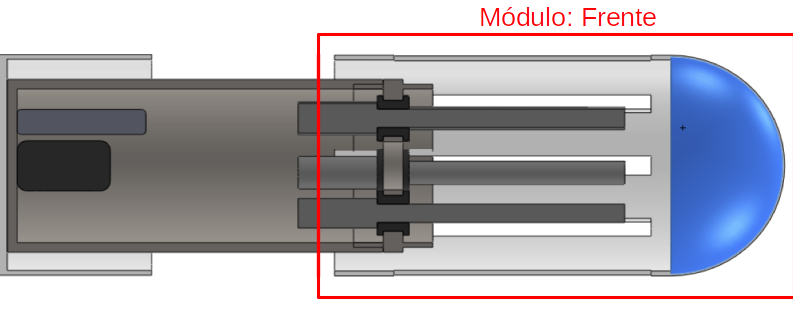
\includegraphics[width=110mm, height=40mm]{Imagenes/cap3/CompletoV5_Frente.png}
        \caption[Corte Transversal]{Corte Transversal Sonda. M\'odulo: Frente.}\textbf{Fuente:} Elaboración Propia.
        \label{fig:Frente}
    \end{figure}
    \item \textbf{Base}: Este m\'odulo, es la parte posterior de la sonda, su función principal es de almacenar de forma segura todo el equipamiento electr\'onico de control, el\'ectrico, almentaci\'on y placas necesarias para los sensores, tal como se indica en la figura \ref{fig:Base2020}, la base est\'a conformada por un cilindro hueco de 270 [mm] de altura, 120[mm] de di\'ametro exterior, espesor de las paredes internas laterales de 10[mm] y un espesor de la base 15[mm],  para sellar de forma herm\'etica, se utilizó un roscado Whitworth fino, utilizada para tuber\'ias de gas y de agua\cite{falk_metalotecnia_1986}, de paso 1,154 [mm].
    
    \begin{figure}[h]
    \centering
    \fbox{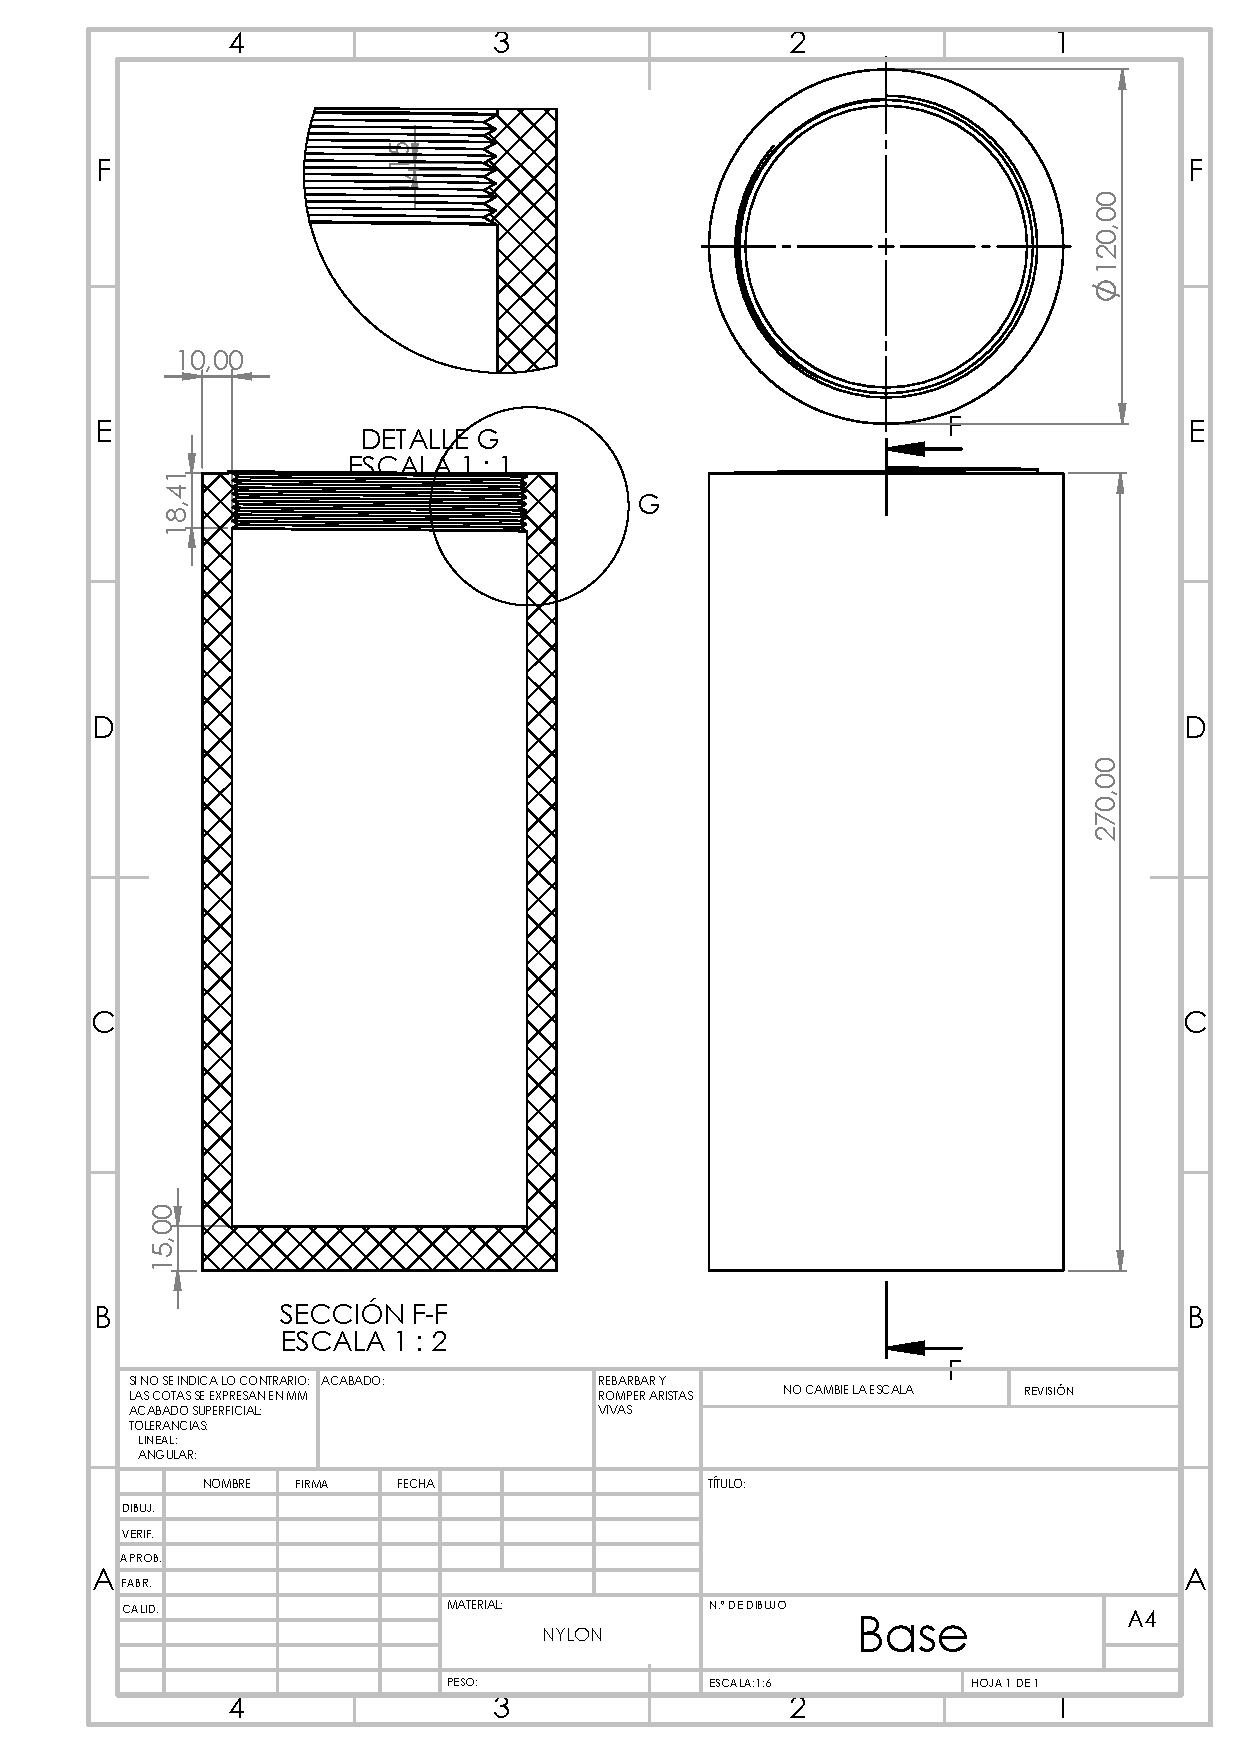
\includegraphics[scale=0.45]{Imagenes/2019/Base2019.PDF} }
    \caption{Dise\~no final de la base. \textbf{Fuente}: Elaboraci\'on propia}
    \label{fig:Base2020}
    \end{figure}
    \item \textbf{Anillo}: Tercer m\'odulo, es la parte centrar de la sonda, adem\'as de servir como enlace entre las otras dos piezas, tiene dos funciones principales, en primer lugar acoplarse a la base cerr\'andolo de forma herm\'etica y la segunda de sostener los sensores en sus posiciones fijas en la sonda. Este es el m\'odulo m\'as peque\~no en relaci\'on a las otras dos, se dise\~no de esta forma para ser el \'unico m\'odulo que se espera se tenga que reemplazar en el caso de ser necesario una reconfiguraci\'on u modificaci\'on de los sensores. Tal como se muestra en la figura \ref{fig:Anillo2019} el dise\~no parte de un cilindro macizo de 70 [mm] de altura y 120[mm] de di\'ametro exterior, se utiliz\'o Whitworth fino al igual que la base a fin de que pueda enroscarse  perfectamente, con el roscado se asegura hasta cierto punto el cierre herm\'etico entre los dos m\'odulos, como medida de seguridad extra se introducen los o-ring, para crear otro  sello hermético al momento del contacto entre las dos m\'odulos, con estos dos sistemas se espera que el ingreso de l\'iquidos sea nulo o m\'inimo, para la implementaci\'on de la sonda en este trabajo se utilizaran 5 sensores, y como esta secci\'on es la encargada que mantener en su posici\'on cada uno de los sensores, se realizan cinco perforaciones en este m\'odulo a fin de poder colocarlos de forma perpendicular. Como estas perforaciones para los sensores implicar\'ia posibles en \'areas de ingreso de l\'iquido, considerando adem\'as que el uso de o-ring se tornan un poco complicados para la posterior fabricaci\'on, se opt\'o por utilizar juntas hidr\'aulicas estandarizadas con el di\'ametro interno compatible con el di\'ametro del los sensores, dispuesta en pares por cada uno de los sensores a fin de 
    
    \begin{figure}[h]
    \centering
    \fbox{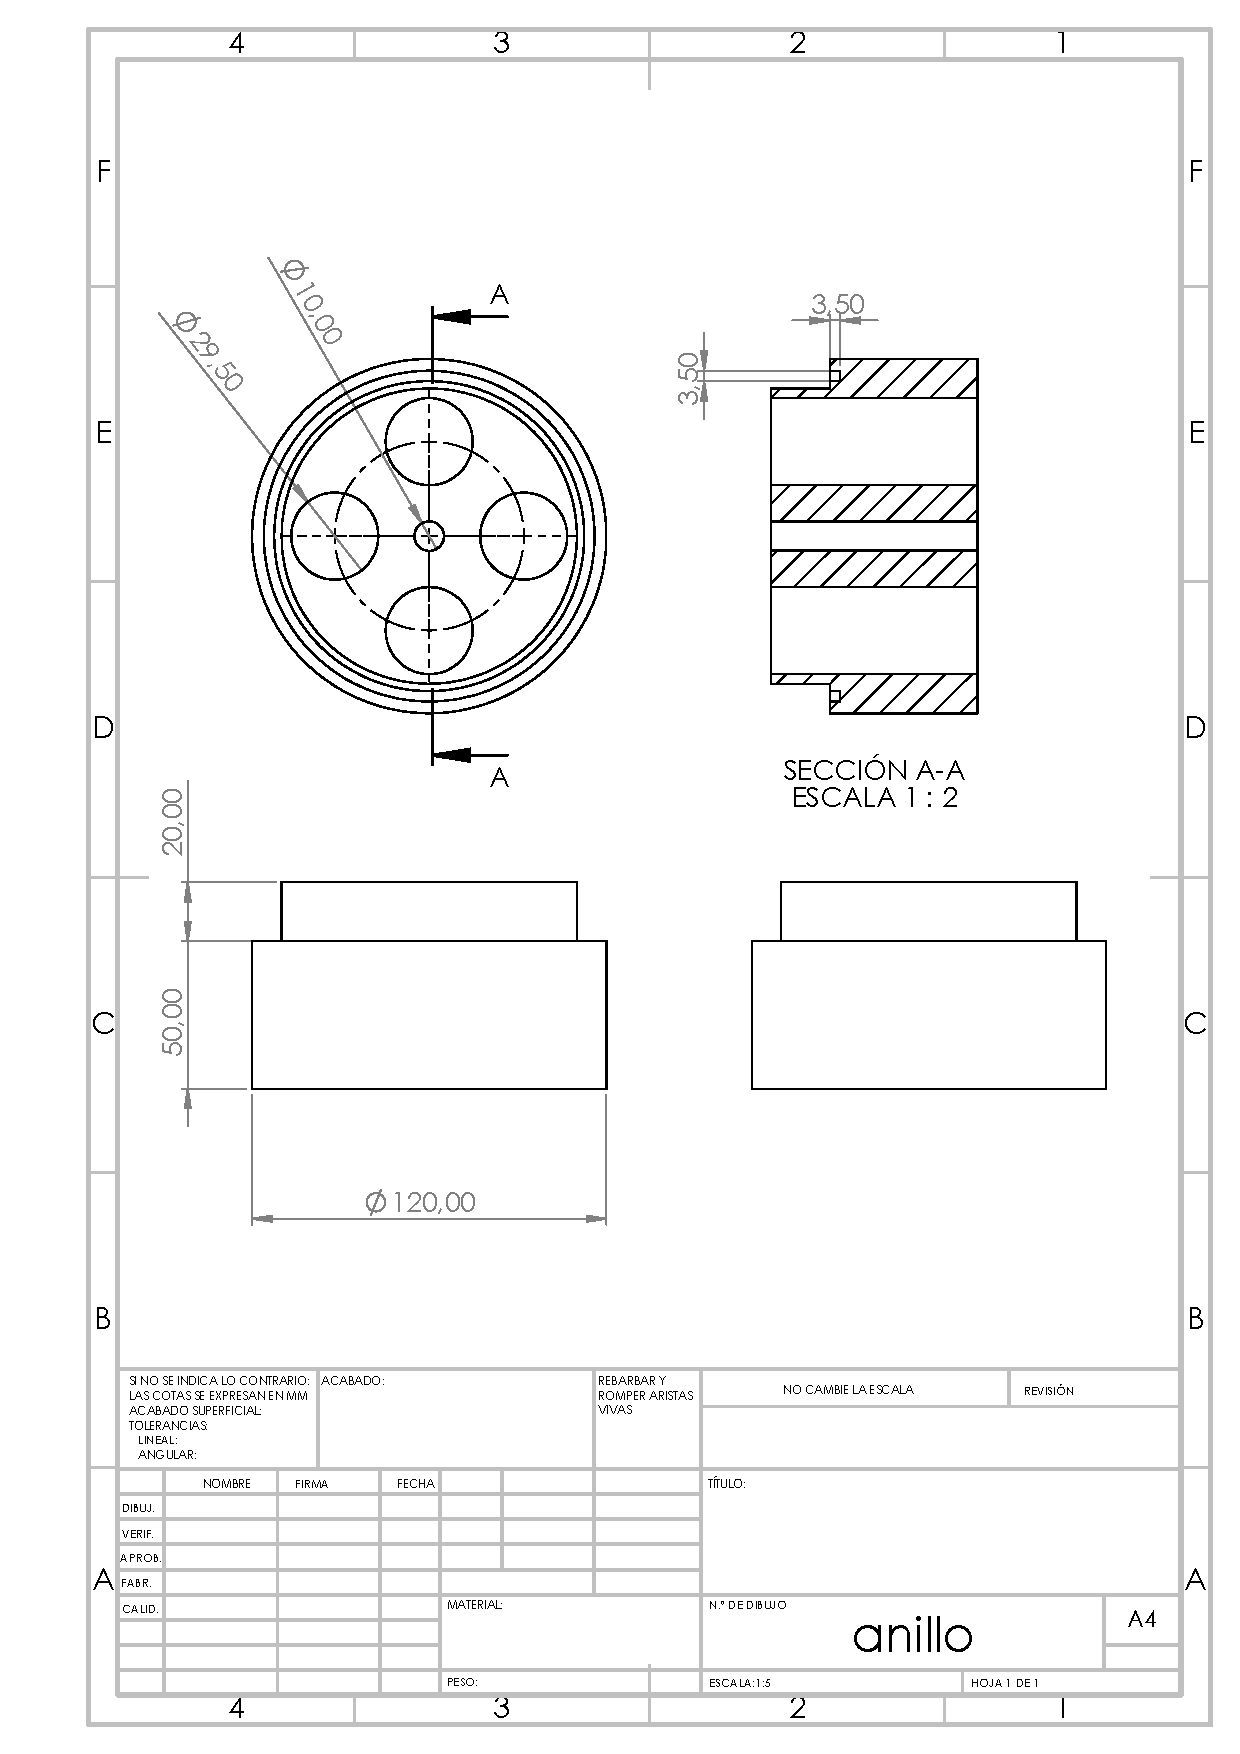
\includegraphics[scale=0.6]{Imagenes/2019/anillo2019.PDF} }
    \caption{Dise\~no final del anillo. Fuente: elaboración propia}
    \label{fig:Anillo2019}
    \end{figure}
\end{itemize}

\subsubsection[Batimetr\'ia]{Batimetr\'ia}
Este subsistema auxiliar, está pensado por la capacidad de medici\'on a multi niveles, cuando se requiera que la sonda descienda el subsistema se encargara de censar la profundidad en el punto de descenso y mandar la informaci\'on a la sonda para seteo de la carrera de la gr\'ua. Se opt\'o por una estructura simple, de bajo costo,  modular y vers\'atil para varios modos de uso.  
La estructura est\'a compuesta por

\subsubsection[Gr\'ua ]{Gr\'ua}


\subsection[Dise\~no El\'ectrico]{Dise\~no El\'ectrico}
\subsubsection[Sonda]{Sonda}
Para lograr autonom\'ia energ\'etica para la sonda se opto por utilizar bater\'ias LiPo Nano-Tech por sus caracter\'isticas t\'ecnicas que permitir\'an alimentar de forma suficiente a toda los componentes que conforman la sonda, como se aprecia en la Figura \ref{fig:4.17}. 

Las baterias Turnigy nano-tech Lipoly bater\'ias fueron dise\~nados para alto rendimiento . Utilizando un avanzado sustrato electrones que permite pasar m\'as libremente de \'anodo a c\'atodo con menos impedancia interna.
 Las ventajas que presenta la utilización de esta fuente son la posibilidad de tener tensiones de +/- 3.3V, +/-5V y +/-12V sin la necesidad de realizar circuitos para la obtención de estos voltajes en comparación a la utilización de baterías de litio.
 \newline
 \hfill
Las ventajas sobre las bater\'ias tradicionales LIPOLY;
\begin{itemize}
    \item La densidad de potencia alcanza 7,5 kW / kg.
    \item Menos hueco de tensi\'on durante la descarga de alta velocidad, dando m\'as poder bajo carga.
    \item Impedancia interna puede llegar tan bajo como 1.2 m${\Omega }$ en comparación con la de 3 m${\Omega }$ de un Lipoly estándar
    \item Control t\'ermico m\'as, paquete por lo general no supera 60 $^{\circ}$C.
    \item Hinchazón durante la carga pesada no supera 5\%, en comparación con 15\% de un Lipoly normal.
    \item Mayor capacidad durante la descarga pesada. M\'as del 90\% a la tasa de 10O\% C.
    \item Carga r\'apida capaz, hasta 15$^{\circ}$C en algunas baterías.
    \item Mayor duraci\'on del ciclo, casi el doble que el de la tecnolog\'ia LiPoly est\'andar.
\end{itemize}


La tecnolog\'ia de nano-core en las bater\'ias de litio es la aplicaci\'on de aditivos conductores nan\'ometros. Los aditivos nan\'ometros conductora forman redes ultra-fuertes de electrones de conducci\'on en los electrodos que pueden aumentar la conductividad electr\'onica.

Estos aditivos crean la capacidad de imbibici\'on en el l\'iquido portador para suministrar m\'as canales de iones. Esto mejora la capacidad de transmisi\'on de iones y la difusi\'on de iones. A trav\'es de la mejora de la conductividad y de iones de transmisi\'on electr\'onica, la impedancia se reduce y la polarizaci\'on de la descarga de alta tasa disminuye en gran medida.

\hfill
\begin{table}[t]
\protect\caption[Caracter\'isticas de bater\'ia Lipo Nano-Tech ]{Caracter\'isticas de bater\'ia Lipo Nano-Tec 5100mAh.}
\label{tab:caract_bat}
\begin{center}
\begin{tabular}{|l|l|}
\hline
Capacidad    &  5100 mAh \\
\hline
Voltaje      &  2S3P/ 7.4 V \\
\hline
Descarga &  65C / 135C \\
\hline
Peso  & 290 g\\
\hline
Dimensi\'on   &  69x47x25 mm\\
\hline
Conector equilibrio	& JST\\
\hline
\end{tabular}
\vspace{5mm}
\newline
\hfill \textbf{Fuente:} P\'agina Web del Fabricante\cite{bateria}
\end{center}
\end{table}

En contrapartida, limitará a nuestro sistema, ya que deberá ir conectado a la red eléctrica todo el tiempo que se requiera del uso de la misma.
\section[Características Técnicas de los módulos]{Características Técnicas del módulo Sonda}
La Tabla \ref{tab:carac_general} detalla las características técnicas del mecanismo a ser desarrollado, teniendo en cuenta los objetivos planteados en la Sección 1.3.

\begin{table}[H]
\protect\caption[Datos Técnicos]{Datos Técnicos. \label{tab:carac_general}}
    \centering
    \scalebox{0.9}{\begin{tabular}{|c|c|}
        \hline
        \textbf{Característica} & \textbf{Valor}  \\
        \hline
        \multicolumn{2}{|c|}{\textbf{Sensores}} \\
        \hline
        Cantidad & $ 5 $   \\
        \hline
        \multicolumn{2}{|c|}{\textbf{Físico}} \\
        \hline
        Dimensiones & $< 50 [cm]$  $< \phi 15[cm]$   \\
        \hline
        Peso &  $ > 6 kg$ \\
        \hline
        Caja Electrónica & Herm\'etica  \\
        \hline
        \multicolumn{2}{|c|}{\textbf{Eléctrico}} \\
        \hline
         Alimentación & 5 V DC  \\
        \hline
         Autonomía & LiPo 5100mAh  \\
        \hline
         \multicolumn{2}{|c|}{\textbf{Interfaz}} \\
         \hline
         Configuración de Parámetros & Por Interfaz Gráfica, SSH, VNC  \\
        \hline
         Transmisi\'on Remota  & Si  \\
        \hline
    \end{tabular}}
    \vspace{5mm}
    \newline
    \hfill \textbf{Fuente:} Elaboración Propia
\end{table}

\subsubsection[Batimetr\'ia]{Batimetr\'ia}
\subsubsection[Gr\'ua ]{Gr\'ua}


\subsection[Dise\~no Electr\'onico]{Dise\~no Electr\'onico}
\subsubsection[Sonda]{Sonda}
\paragraph[Interfaz de Sensores]{Interfaz de Sensores}
Es el bloque donde se obtiene las mediciones de las caracter\'isticas f\'isico - qu\'imica del recurso h\'idrica, para su posterior procesamiento, almacenamiento y transmici\'on a base remoto.

\subparagraph{Sensor de pH}
En la Figura \ref{fig:4.8} se puede apreciar el sensor de pH por el que se optó fabricado por la empresa Atlas Scientfic.
    \begin{figure}[t]
    \centering
	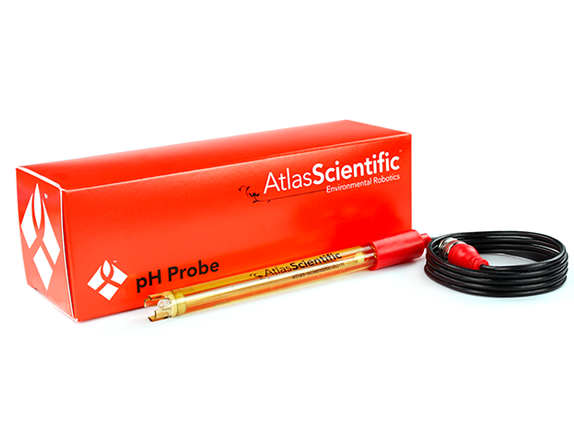
\includegraphics[width=150mm, height=90mm]{Imagenes/2021/imag23.png}%\textwidth%
	\caption[Sonda de pH de la empresa Atlas Scientific]{Sonda de pH de la empresa Atlas Scientific. \textbf{Fuente:} Página Web del fabricante.}
	\label{fig:4.8}
    \end{figure}
Los criterios para la selección de este sensor fueron, su simplicidad de uso gracias a su extensa documentación y soporte por parte del fabricante, su popularidad en el ámbito de la automatización y control de calidad de agua para varios tipos de usos y su integración dentro de la placa de desarrollo sin necesidad de cableados externos y compatible con el módulo EZO pH Circuit que se muestra en la Figura \ref{fig:4.9}
\newline
\hfill
    \begin{figure}[H]
    \centering
	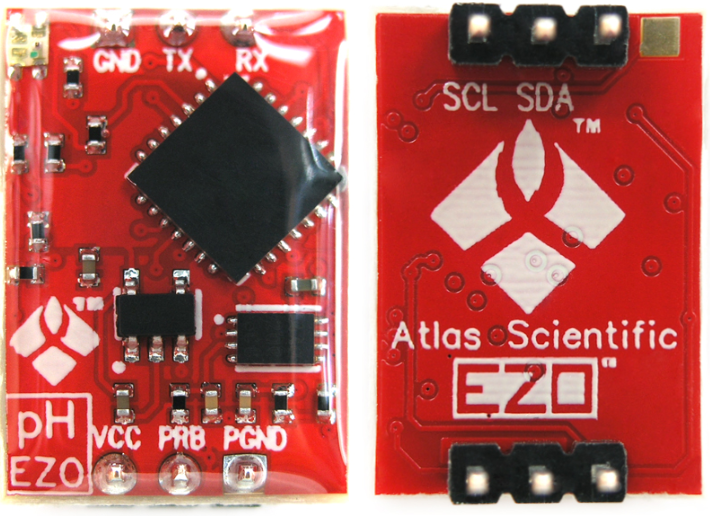
\includegraphics[width=70mm, height=60mm]{Imagenes/2021/imag27.png}%\textwidth%
	\caption[EZO pH Circuit]{EZO pH Circuit.\textbf{Fuente:} Pagina Web del Fabricante.}
	\label{fig:4.9}
    \end{figure}
El módulo es un dispositivo bastante sensible, y ésta sensibilidad es lo que le da una excelente precisión. Significa que es capaz de leer microvoltajes que están presentes en el agua de fuentes no naturales como bombas, válvulas de solenoide u otras sondas o sensores lo que ocasiona lecturas que fluctúan rápidamente o lecturas que están constantemente apagadas.

Al leer el pH y la conductividad u oxígeno disuelto juntos, el fabricante recomienda que los módulos estén aislados eléctricamente de los demás circuitos, subsanados con el la placa de Tentacle.
\newline
\hfill
\begin{figure}[t]
    \centering
    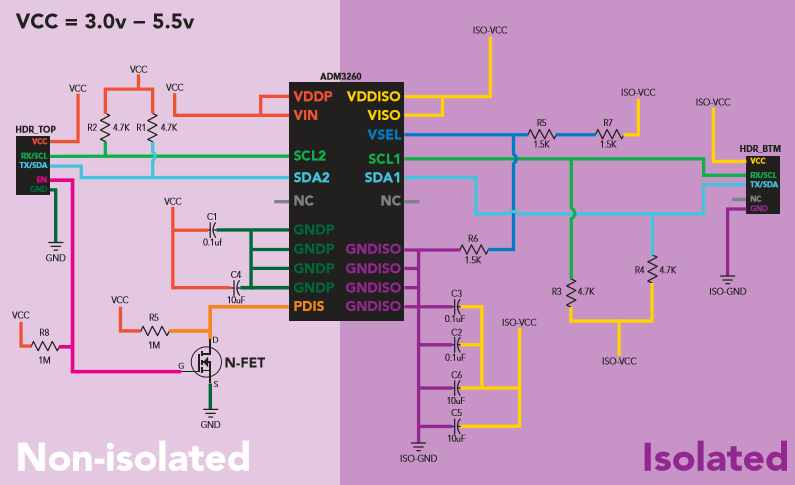
\includegraphics[width=150mm, height=90mm]{Imagenes/2021/imag36.png}
    \caption[Esquema de Funcionamiento del circuito EZO pH]{Esquema de Funcionamiento del circuito EZO pH.\textbf{Fuente: }Pagina Web del Fabricante\cite{ezoph}.}
    \label{fig:4.10}
\end{figure}
En la Figura \ref{fig:4.10} se muestra  el esquema del circuito interno del módulo, cómo están aislados datos y la potencia con el ADM3260, que es el chip encargado de realizar la aislación de los canales I2C utilizados y algunos componentes pasivos. El ADM3260 puede generar una potencia aislada de hasta 150 mW e incorpora dos canales de datos bidireccionales.
Esta tecnología funciona mediante el uso de pequeños transformadores para inducir el voltaje a través de un espacio de aire. Los dos canales de datos tienen una resistencia de extracción de 4.7 k$\Omega$ tanto en las líneas aisladas como en las no aisladas (R1, R2, R3 y R4). El voltaje de salida se configura mediante un divisor de voltaje (R5, R6 y R, 7). produce un voltaje de 3.9V independientemente de su voltaje de entrada.


\textbf{Principio de Operación: }Una sonda de pH mide la actividad del ion de hidrógeno en un líquido, en el extremo inferior de ésta hay una membrana de vidrio que permite a los iones de hidrógeno del líquido que se está midiendo depositarse en la capa exterior del vidrio, mientras que los iones más grandes permanecen en la solución. En la Figura \ref{fig:4.11} se pude apreciar el comportamiento de los iones de hidrógeno de acuerdo al tipo de solución que se tiene. La diferencia en la concentración de iones de hidrógeno (fuera de la sonda y en el interior de la sonda) crea una corriente muy pequeña. Esta corriente es proporcional a la concentración de iones de hidrógeno en el líquido que se mide.
La corriente que se genera a partir de la actividad del ion hidrógeno es el recíproco de esa actividad y se puede predecir usando esta ecuación:
\begin{equation}
E=E^0 + \frac{RT}{F}\times \ln\alpha_{H+} = E^0 - \frac{2.303RT}{F}\rho H
\label{eq:iv}
\end{equation}
Donde $R$ es la constante ideal del gas, $T$ es la temperatura en grados Kelvin y $F$ es la constante de Faraday.
\newline
\hfill
\begin{figure}[t]
\centering
	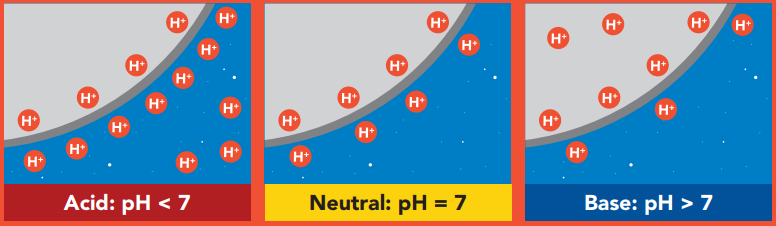
\includegraphics[width=160mm, height=70mm]{Imagenes/2021/imag22.png}%\textwidth%
	\caption[Actividad de los iones de hidrógeno]{Actividad de los iones de hidrógeno.  \textbf{Fuente:}Pagina Web del Fabricante \cite{atlasph}}
	\label{fig:4.11}
\end{figure}

En la Tabla \ref{tab: caract_sondaph} se detallan las características del sensor de pH.
\newline
\hfill
Entre las aplicaciones típicas en las que se utiliza esta sonda están, uso estándar de laboratorio, uso en el campo, en el suelo, cultivos con técnicas de hidroponía o acuaponía, muestras que contienen metales pesados,cerveza, vino y otros.

\begin{table}[H]
\protect\caption[Características del sensor de pH de AtlasScientific]{Características del sensor de pH de AtlasScientific.}
\label{tab: caract_sondaph}
\begin{center}
\begin{tabular}{|l|l|}
\hline
Rango    &  0 - 14\\
\hline
Exactitud      &  +/-0.002\\
\hline
Conector &  BNC macho\\
\hline
Resolución   &  +/-0.0001\\
\hline
Tiempo de Respuesta   &  95\% en 1s\\
\hline
Presión Máxima    &  100PSI\\
\hline
Profundidad Máxima	& 60m\\
\hline
Rango de Temperatura $^{\circ}$C	& 1- 99\\
\hline
Longitud del Cable	& 1m\\
\hline
Sensor de Temperatura Interno	& NO\\
\hline
Tiempo antes de recalibración	& 1 año\\
\hline
Tiempo de Vida	& aprox. 2.5 años\\
\hline
Seguro en Alimentos & Si\\
\hline
Peso & 49 gramos\\
\hline
Dimensiones & 12mm x 150 mm\\
\hline
\end{tabular}
\vspace{5mm}
\newline
\hfill
\textbf{Fuente: }Pagina Web del Fabricante\cite{atlasph}
\end{center}
\end{table} 


\subparagraph{Sensor de Conductividad}
El sensor utilizado para las lecturas de conductividad se puede apreciar en la Figura \ref{fig:4.12}, también de la empresa Atlas Scientific.
\begin{figure}[t]
\centering
	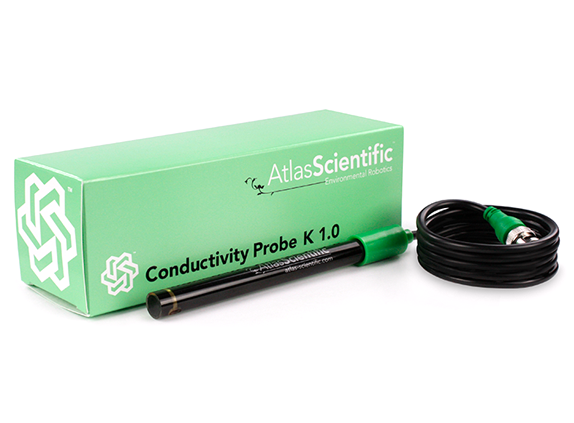
\includegraphics[width=150mm, height=90mm]{Imagenes/2021/imag24.png}%\textwidth%
	\caption[Sensor de CE]{Sensor de CE.  \textbf{Fuente:}Pagina Web del Fabricante \cite{atlasce}}
	\label{fig:4.12}
\end{figure}
Los criterios de selección fueron su extendido uso para control de calidad de aguas para varios usos, buen soporte y extensa documentación disponible en la web, la homogeneidad en los dispositivos electrónicos, al utilizar sensores ya compatibles (Sensor de pH y Sensor de CE) y con los debidos aislamientos requeridos entre estos.  
 
El módulo EZO conductivity Circuit, se muestra en la Figura \ref{fig:4.13} emplea un método de resolución de escala. A medida que aumenta la conductividad, la resolución entre lecturas disminuye como se puede apreciar en la Tabla \ref{tab:resol_ce}.
\begin{figure}[b]
    \centering
    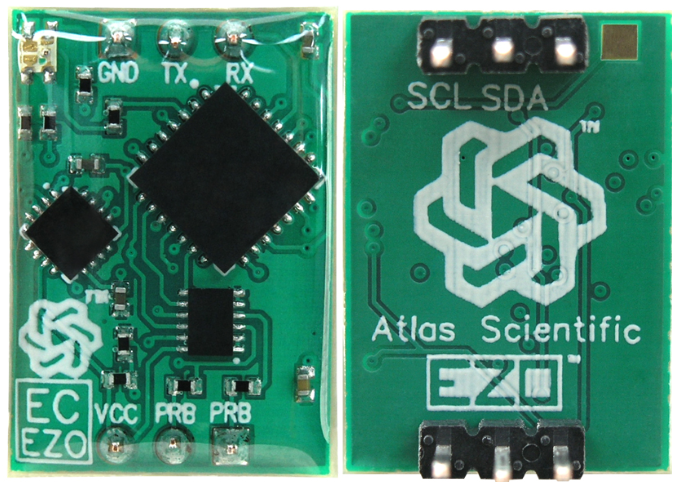
\includegraphics[width=70mm, height=60mm]{Imagenes/2021/imag28.png}
    \caption[EZO conductivity Circuit]{EZO conductivity Circuit. \textbf{Fuente: }Página Web del Fabricante.}
    \label{fig:4.13}
\end{figure}
El módulo emitirá lecturas de conductividad donde los primeros 4 dígitos son válidos y los demás se establecen en 0. Esto excluye las lecturas de conductividad que son menores a 9.99. En ese caso, solo se emitirán 3 dígitos de conductividad.

\begin{table}[t]
    \label{tab:resol_ce}
    \protect\caption[Resolución de Escala Sensor de Conductividad]{Resolución de Escala Sensor de Conductividad.}
    \centering
    \begin{tabular}{ c c }
         \toprule
         \textbf{Valor}&\textbf{Resolución}  \\
         \midrule
%         \hline
         0.07-99.99 & 0.01$ \mu S/cm$ \\
%         \hline
         100.1-999.9 & 0.1 $\mu S/cm $\\
%         \hline
         1,000-9,999 & 1.0 $\mu S/cm$ \\
%         \hline
         10,000-99,990 & 10.0 $\mu S/cm $\\
%         \hline
         100,000-999,99 & 100 $\mu S/cm$ \\
%         \hline
        \bottomrule
    \end{tabular}
   \vspace{5mm}
   \newline
    \textbf{Fuente: }\cite{ezoce}.
\end{table}




\textbf{Principio de operación: }
Una sonda de conductividad eléctrica (CE) mide la conductividad eléctrica en una solución. Se usa comúnmente en ecosistemas de agua dulce para controlar la cantidad de nutrientes, sales o impurezas en el agua.
Dentro de la sonda de conductividad, dos electrodos se colocan opuestos entre sí como se muestra en la Figura \ref{fig:4.14}, se aplica un voltaje de CA a los electrodos, lo que hace que los cationes se muevan al electrodo cargado negativamente, mientras que los aniones se mueven al electrodo positivo. Cuanto más electrolito libre contiene el líquido, mayor es la conductividad eléctrica.

\begin{figure}[H]
    \centering
    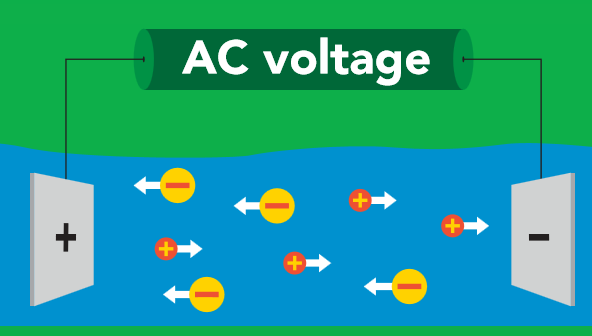
\includegraphics[width=90mm, height=60mm]{Imagenes/2021/imag37.png}
    \caption[Principio de Funcionamiento del Sensor de Conductividad]{Principio de Funcionamiento del Sensor de Conductividad. \textbf{Fuente: }\cite{ezoce}.}
    \label{fig:4.14}
\end{figure}

En la Tabla \ref{tab:caract_ce} se muestran las principales características del sensor de conductividad.
Entre los usos comunes de este sensor se encuentran el uso estándar en laboratorio, uso en el campo, en acuaponía, hidroponía y en acuarios.
\begin{table}[H]
\protect\caption[Características del sensor de CE de AtlasScientific]{Características del sensor de CE de AtlasScientific.}
\label{tab:caract_ce}
\begin{center}
\begin{tabular}{|l|l|}
\hline
Rango    &  5 - 200.000 $\mu S\/cm$\\
\hline
Exactitud      &  +/-2\% \\
\hline
Conector &  BNC macho\\
\hline
Resolución   &  +/-0.0001\\
\hline
Tiempo de Respuesta   &  90\% en 1s\\
\hline
Presión Máxima    &  3,447 kPa (500 PSI) \\
\hline
Profundidad Máxima	& 343 metros\\
\hline
Rango de Temperatura $^{\circ}$C	& 1- 110\\
\hline
Longitud del Cable	& 1m\\
\hline
Sensor de Temperatura Interno	& NO\\
\hline
Tiempo antes de recalibración	& 10 año\\
\hline
Tiempo de Vida	& aprox. 10 años\\
\hline
Dimensiones	& 12mm x 152mm\\
\hline
Peso	& 51 gramos\\
\hline
Superficie de medición	& Grafito\\
\hline
Seguro en Alimentos	& Si\\
\hline
\end{tabular}
\vspace{5mm}
\newline
\hfill \textbf{Fuente:} \cite{atlasce}
\end{center}
\end{table}

%%%%%%%%%%%%%%%%%%%%%%%%CAMBIAR
\subparagraph{Sensor de Temperatura}
En la Figura \ref{fig:4.15}  se puede apreciar el sensor de Temperatura utilizado fabricado por la empresa Atlas Scientific.


\begin{figure}[t]
    \centering
    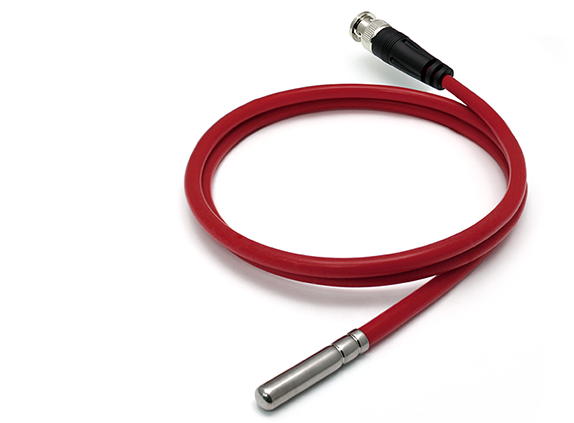
\includegraphics[width=90mm, height=70mm]{Imagenes/2021/imag39.png}
    \caption[Sensor de Temperatura PT 1000]{Sensor de Temperatura PT 1000. \textbf{Fuente: } Página Web del Fabricante. }
    \label{fig:4.15}
\end{figure}


\textbf{Principio de Operación: }
A diferencia de cualquier otro material, la correlación entre la resistencia y la temperatura en el platino es bastante lineal. Es por esta razón que el sensor de temperatura RTD de platino es el estándar industrial para la medición de temperatura.

La sonda de temperatura PT-1000 es un termómetro tipo resistencia. Donde PT significa platino y 1000 es la resistencia medida de la sonda a 0$^{\circ}$C en $\Omega$ (1k a 0$^{\circ}$C).
A medida que la temperatura cambia, la resistencia del platino cambia.
Para convertir la resistencia de la sonda a la temperatura, se utiliza la siguiente ecuación simplificada

\begin{equation}
    T=-\frac{\sqrt{(-0.00232(R)+17.59246)}-3.908}{0.00116}
\end{equation}

Donde $T$ esta en grados Celsius y $R$ es el valor de la resistencia medida por el sensor.

El módulo utilizado para el tratamiento de las señales es el mostrado en la Figura \ref{fig:4.16} también fabricado por la empresa Atlas Scientific.

\begin{figure}[t]
    \centering
    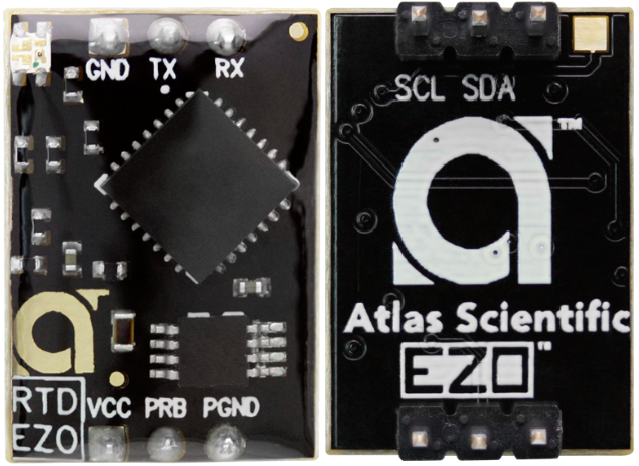
\includegraphics[width=90mm, height=70mm]{Imagenes/2021/imag38.png}
    \caption[EZO-RTD Circuito Integrado de Temperatura]{EZO-RTD Circuito Integrado de Temperatura.\textbf{Fuente: }Pagina Web del Fabricante.}
    \label{fig:4.16}
\end{figure}

Es un sistema informático de tamaño reducido que está diseñado específicamente para ser utilizado en aplicaciones donde se requiera mediciones exactas y precisas de la temperatura a través de una sonda de temperatura genérica PT-100 / PT-1000. Se conecta directamente a la placa Tentacle T3 y no necesita de aislamiento a diferencia de los otros módulos de sensores.

En la Tabla \ref{tab:caract_temp} se visualizan las características del Sensor de Temperatura PT-1000.
Entre las aplicaciones de uso común de este sensor están el uso estándar de laboratorio, uso en el campo, en el suelo, acuapon\'ia, hidroponía, en bebidas como cerveza, vino u otro licor.

% Sensor REDOX
% Sensor OD


\textbf{Bloque de Control}
Este bloque es el encargado de realizar el procesamiento de los datos recibidos a través de los sensores y la configuración de parámetros adquirida por la Interfaz de Usuario.

\begin{itemize}
    \item \textbf{Hardware:}
    En la Figura \ref{fig:4.4} se observa la placa de desarrollo low cost escogida para el presente proyecto, la Raspberry Pi 3 model B desarrollado por la fundación Raspberry Pi. La misma cuenta con un procesador multimedia Broadcom BCM2835 system-on-chip (SoC).
    \newline
    \hfill
    La CPU Contiene un ARM1176JZFS, con unidad de coma flotante, que funciona a 700Mhz y es capaz de soportar overclock a 1GHZ en modo “TURBO” que hace que el SoC de más rendimiento sin reducir el tiempo de vida de la placa y sin perder la garantía. 
    La memoria RAM es de 512MB de SDRAM (en su modelo B), en un único módulo, el cual, funciona a 400Mhz en su modo normal y alcanzando los 600Mhz en su versión “TURBO”.
    La  Raspberry Pi no tiene un disco duro tradicional, para ello dispone de un lector para memorias SD, un sistema de almacenamiento en estado sólido. El arranque del sistema se hará desde la propia tarjeta SD, con lo que, debido a que tiene que albergar todo el sistema operativo, es necesario que la tarjeta sea de al menos 2 GB de capacidad para almacenar todos los archivos requeridos.
    La placa carece de botón de encendido y apagado, con lo que la energía le llega mediante un conector microUSB estándar de 5V. El consumo de la placa es de 700mA, (3,5W).
    La Raspberry Pi, está diseñada para ejecutar el sistema operativo GNU/Linux y la version mas extendido es el Raspberry Pi OS .
    \begin{figure}[t]
        \centering
        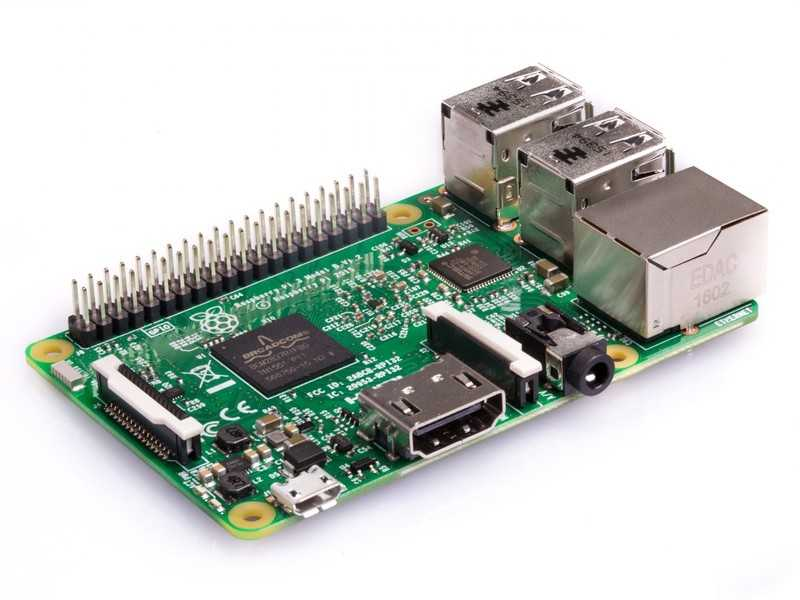
\includegraphics[width=100mm, height=70mm]{Imagenes/2021/imag35.jpg}
        \caption[Placa Raspberry Pi 3 model B]{Placa Raspberry Pi 3 model B.\textbf{Fuente:} Página Web del Fabricante.}
        \label{fig:4.4}
    \end{figure}

    Se optó por este controlador por sus prestaciones,  t\'ecnicas, suficientes para las tareas a ser ejecutadas, con un almacenamiento externa de 64 Gb con una memoria tipo microSD de alto rendimiento, por sus dimensiones reducidas, la raspberry  eran acorde a los requerimientos necesarios y por tener un gran soporte y comunidad activa en l\'inea.
 
    En la Tabla \ref{tab:carac_rasp} se detallan las principales características técnicas de la Raspberry Pi 3 model B.
 
 \begin{table}[t]
      \protect\caption[Características Técnicas. Raspberry Pi 3 model B]{Características Técnicas. Raspberry Pi 3 model B.  \label{tab:carac_rasp}}
    
     \centering
     \begin{tabular}{l c}
        \toprule
           Sistema Operativo & Raspberry Pi OS\\
%          \hline
          Juego de Instrucciones & RISC 64 bits\\
%          \hline
          Procesador & RQuad Core 1.2GHz Broadcom BCM2837\\
%          \hline
          RAM  & 1 GB\\
%          \hline
          Bluetooth &  4.2 Low Energy (BLE)\\
%          \hline
          Puertos USB 2.0 & 4\\
%          \hline
          GPIO& 40\\
%          \hline
          UART& 2\\
%          \hline
          I2C& 4\\
%          \hline
          Stero/Video & 1\\
%          \hline
          HDMI & 1\\
%          \hline
          CSI(RPI Camera) & 1\\
%          \hline
          DSI(RSP Touchscreen display) & 1\\
%          \hline
          Dimensiones & 85.60 mm x 53.98 mm\\
%          \hline
          Peso & 50 g\\
%          \hline
          Consumo energ\'etico & 4 W\\
%          \hline
          Alimentaci\'on & 5 V\\
%          \hline
     \bottomrule   
     \end{tabular}
     \vspace{5mm}
     \newline
     \hfill \textbf{Fuente:} Elaboración Propia. Información recopilada de \cite{rasp}
\end{table}
    Por otra parte, para eliminar la necesidad de cableado, multiplexación y aislamiento eléctrico en la lectura de los sensores, se optó por la utilización de la placa open source Tentacle Shield para arduino de Whitebox labs, la cual se muestra en la Figura \ref{fig:4.5}.
\begin{figure}[t]
    \centering
    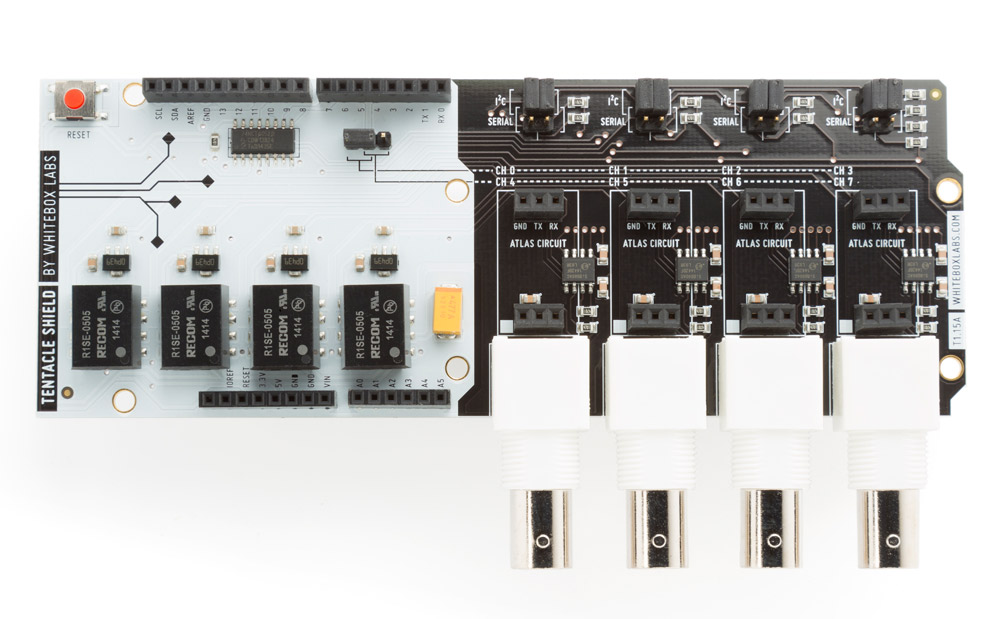
\includegraphics[width=100mm, height=70mm]{{Imagenes/2021/imag26.jpg}}
    \caption[Placa Tentacle para Arduino]{Placa Tentacle para Arduino. \textbf{Fuente:} Página web del Fabricante}
    \label{fig:4.5}
\end{figure}

    Es una forma pr\'actica y fácil de leer múltiples sensores de la empresa Atlas Scientific, la placa puede alojar hasta 4 dispositivos EZO de Atlas Scientific para medir pH(Potencial de Hidrógeno), Oxígeno Disuelto(DO por sus siglas en inglés), conductividad eléctrica(CE), Temperatura(T), Potencial de Reducción de Oxidación(ORP por sus siglas en inglés)

    \textbf{Aislamiento:}
    Los circuitos de medición y las líneas de comunicación aislados individualmente evitan el ruido y los bucles de tierra para obtener mediciones precisas, incluso en sistemas de bucle cerrado.Los sensores no interferirán entre sí y la mayoría del ruido eléctrico exterior que puede interferir con las lecturas se reducirá.

    \item \textbf{Software:}El software de control fue desarrollado en el lenguaje de programación Python. Este es un lenguaje interpretado multiparadigma, soporta programación orientada a objetos, imperativa y funcional.
    Python ya viene instalado en el sistema operativo Raspberry Pi OS para Raspberry Pi.Tiene la ventaja de poder utilizar los pines GPIO de la placa de desarrollo para conectar el mundo digital con el mundo físico mediante la programación, facilitando de esta manera el control de la lectura de los distintos sensores y el accionamiento de los actuadores utilizados.
    
    El administrador de Base de Datos utilizado fue Sqlite3, es un sistema de gestión de base de datos ampliamente difundido en el mundo de la programación de aplicaciones móviles.
    La utilización de este gestor fue debido a su gran portabilidad y su capacidad  de gestionar bases de datos de hasta 2 terabyte de tamaño.
    En la Tabla \ref{tab:caract_sqlite} se muestran las características más relevantes de la Base de Datos Sqlite.

    \begin{table}[H]
    \protect\caption[Características del Gestor de Base de Datos SQLITE]{Características del Gestor de Base de Datos SQLITE.\label{tab:caract_sqlite}}
        \centering
        \begin{tabular}{|l|l|}
            \hline
            Soporte & Múltiples tablas,\textit{triggers} y vistas   \\
            \hline
             Lectura y Escritura& \multicolumn{1}{|l|}{\begin{tabular}[c]{@{}l@{}}  Directamente sobre archivos que se encuentran en el disco \\ duro.\end{tabular}} 
             \\
             \hline
             Formato & 
             \multicolumn{1}{|l|}{\begin{tabular}[c]{@{}l@{}}  Multiplataforma. Puede ser utilizado en sistemas de 32 bits \\ o 64 bits.\end{tabular}} 
           \\
             \hline
             Operaciones &\multicolumn{1}{|l|}{\begin{tabular}[c]{@{}l@{}} Realiza operaciones de manera más eficiente y rápido que  \\ MySql y PostgreSQL.\end{tabular}} 
            \\
             \hline
             Interfaz API &\multicolumn{1}{|l|}{\begin{tabular}[c]{@{}l@{}}Opera con diversas Interfaces API lo que permite trabajar  \\con C++, PHP, Python, Groovy, etc.\end{tabular}} 
            \\
             \hline
             Dependencias Externas & No\\
             \hline
             Librerías & Cuentan con acceso para muchos lenguajes de programación.\\
             \hline
             UDF & Soporta funciones SQL definidas por el usuario.\\
             \hline
             Código Fuente & Dominio público y documentación extensa.\\
             \hline
        
        \end{tabular}
        \vspace{5mm}
        \newline
        \hfill \textbf{Fuente: }P\'agina Web del desarrollador.\cite{sqlite}
        
    \end{table}
    
\end{itemize}
%%%%%%%%%%%%%%%%%%%%%%%%%%%%%%%%%%%%
\subsubsection[Batimetr\'ia]{Batimetr\'ia}
\subsubsection[Gr\'ua ]{Gr\'ua}


\subsection[Dise\~no Control]{Dise\~no Control}
\subsubsection[Sonda]{Sonda}
\begin{table}[t]
\protect\caption[Funciones Generales]{Funciones Generales. \label{tab:fun_general}}
    \centering
    \begin{tabular}{l l l}
        \toprule
        \textbf{Descripción} & \textbf{Decisión} & \textbf{Característica} \\
        \midrule
         Comunicaci\'on  Perif\'ericos  & Algoritmo comunicaci\'on & \multicolumn{1}{ l}{\begin{tabular}[c]{@{}l@{}} Env\'io y recipci\'oon de estados \\ funcionamiento y datos de los \\ dispositivos conectados a la red \end{tabular}}
         \\
%        \hline
        Lectura de Sensores & Algoritmo muestreo & \multicolumn{1}{l}{\begin{tabular}[c]{@{}l@{}} Se Lectura secuencial de los\\ sensores pH, CE,\\ OD, OPR, T\end{tabular}}
         \\
%        \hline
        Almacenamiento datos & Algoritmo datos &
        \multicolumn{1}{l}{\begin{tabular}[c]{@{}l@{}} Consulta y registro as\'incrono \\ 
        del muestreo\end{tabular}}
         \\
%        \hline
        Transmisi\'on datos  & Algoritmo transmisi\'on &
        \multicolumn{1}{l}{\begin{tabular}[c]{@{}l@{}} Transmisi\'on asincr\'onica \\ a estaci\'on remota \end{tabular}}
           \\
        \bottomrule
    \end{tabular}
    \vspace{5mm}
    \newline
    \hfill \textbf{Fuente:} Elaboración Propia
\end{table}
\section{Descripci\'on  sistema }
\section[Descripción General del Sistema]{Descripción General del Sistema}
En referencia al modelo conceptual del sistema, este está constituido, por un bloque interfaz de usuario, un bloque de control, un bloque de sensores, un bloque de actuadores y un bloque de alimentaci\'on,  como se puede apreciar en la Figura \ref{fig:4.1}.
\section[Características Técnicas de los módulos]{Características Técnicas del módulo Despliegue}
La Tabla \ref{tab:carac_general} detalla las características técnicas del mecanismo a ser desarrollado, teniendo en cuenta los objetivos planteados en la Sección 1.3.
\begin{table}[H]
\protect\caption[Datos T\'ecnicos]{Datos T\'ecnicos. \label{tab:carac_general}}
    \centering
    \scalebox{0.9}{\begin{tabular}{|c|c|}
        \hline
        \textbf{Caracter\'istica} & \textbf{Valor}  \\
        \hline
        \multicolumn{2}{|c|}{\textbf{F\'isico}} \\
        \hline
        Capacidad de carga & $ > 10 [Kg] $   \\
        \hline
        Dimensiones & $< 50 [cm]$  x $50 [cm]$ x $50 [cm]$    \\
        \hline
        Peso &  $ < 15 kg$ \\
        \hline
        Caja Electr\'onica & Herm\'etica  \\
        \hline
        \multicolumn{2}{|c|}{\textbf{Eléctrico}} \\
        \hline
         Alimentaci\'on & 12 V DC  \\
        \hline
         Autonom\'ia & No  \\
        \hline
         \multicolumn{2}{|c|}{\textbf{Interfaz}} \\
         \hline
         Configuraci\'on de Par\'ametros & Por Interfaz Gr\'afica  \\
        \hline
         Transmisi\'on Remota  & Si  \\
        \hline
    \end{tabular}}
    \vspace{5mm}
    \newline
    \hfill \textbf{Fuente:} Elaboraci\'on Propia
\end{table}
\subsubsection[Batimetr\'ia]{Batimetr\'ia}
\subsubsection[Gr\'ua ]{Gr\'ua}


\subsection[Dise\~no de Interfaz]{Dise\~no de Interfaz}
\subsubsection[Sonda]{Sonda}
\subsubsection[Batimetr\'ia]{Batimetr\'ia}
\subsubsection[Gr\'ua ]{Gr\'ua}


\section[Fabricaci\'on]{Fabricaci\'on}
\subsubsection[Sonda]{Sonda}
La fabricaci\'on de las partes de la sonda se realiz\'o con dos t\'ecnicas desarrollados en el cap\'itulo anterior, la base y el anillo se realizaron con la t\'ecnica de fabricaci\'on sustractiva de   se realiz\'o en el laboratorio de Metal Mec\'anica de la Facultad de Ingenier\'ia Universidad Nacional de Asunci\'on, con un torno semiatom\'atico, con la t\'ecncia de vaciado progresivo. 
        
\begin{figure}[h]
\centering
\fbox{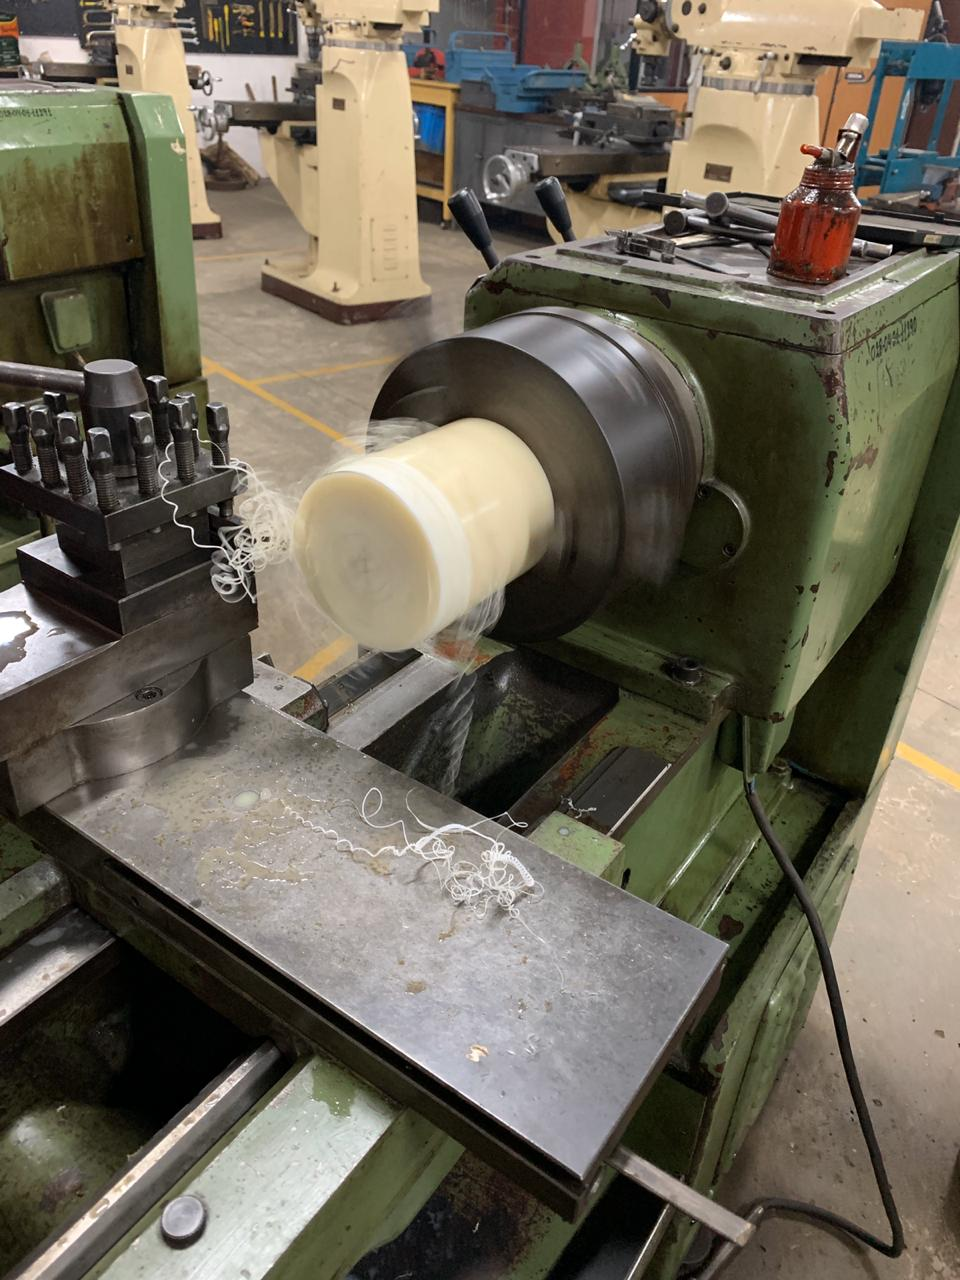
\includegraphics[scale=0.2]{Imagenes/2019/Sonda_Fab0.jpeg} }
\caption{Tubo de Nylon r\'igido en proceso de desgaste. Fuente: elaboración propia}
\label{fig:preparacion}
\end{figure}
 
\hfill\section{Fabricaci\'on de la Sonda.}
\begin{figure}[t]
\centering
\fbox{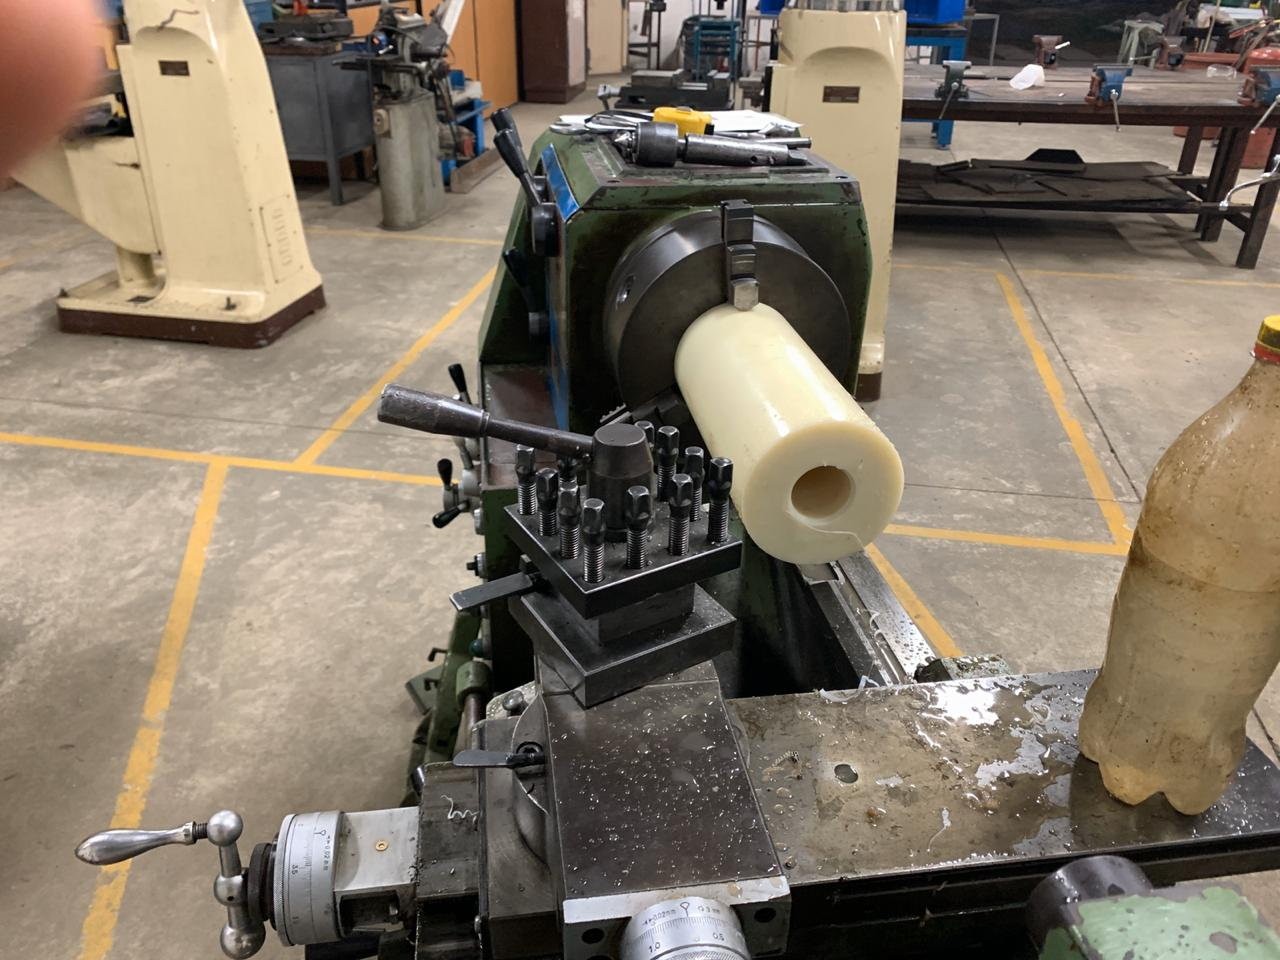
\includegraphics[scale=0.2]{Imagenes/2019/Sonda_Fab.jpeg}}
\caption{Tubo de Nylon r\'igido, proceso de vaciado. Fuente: elaboración propia}
\label{fig:preparacion}
\end{figure}

\subsubsection[batimetría]{Batimetr\'ia} 
Tal como se observa en la figura \ref{fig:batimetro} el sistema de medici\'on de profundidad fue dise\~nado de tal forma que permita ser instalado en la parte posterior (popa) del VAS, mediante dos abrazaderas, uno de su sujeci\'on y otra de sujeci\'on - nivelaci\'on para asegurarse  pueda estar en contacto con el agua al momento de instalarse.  Para la correcta  instalci\'on de se debe alinear el sonar con la parte m\'as baja de la popa 

\begin{figure}[h]
\centering
\fbox{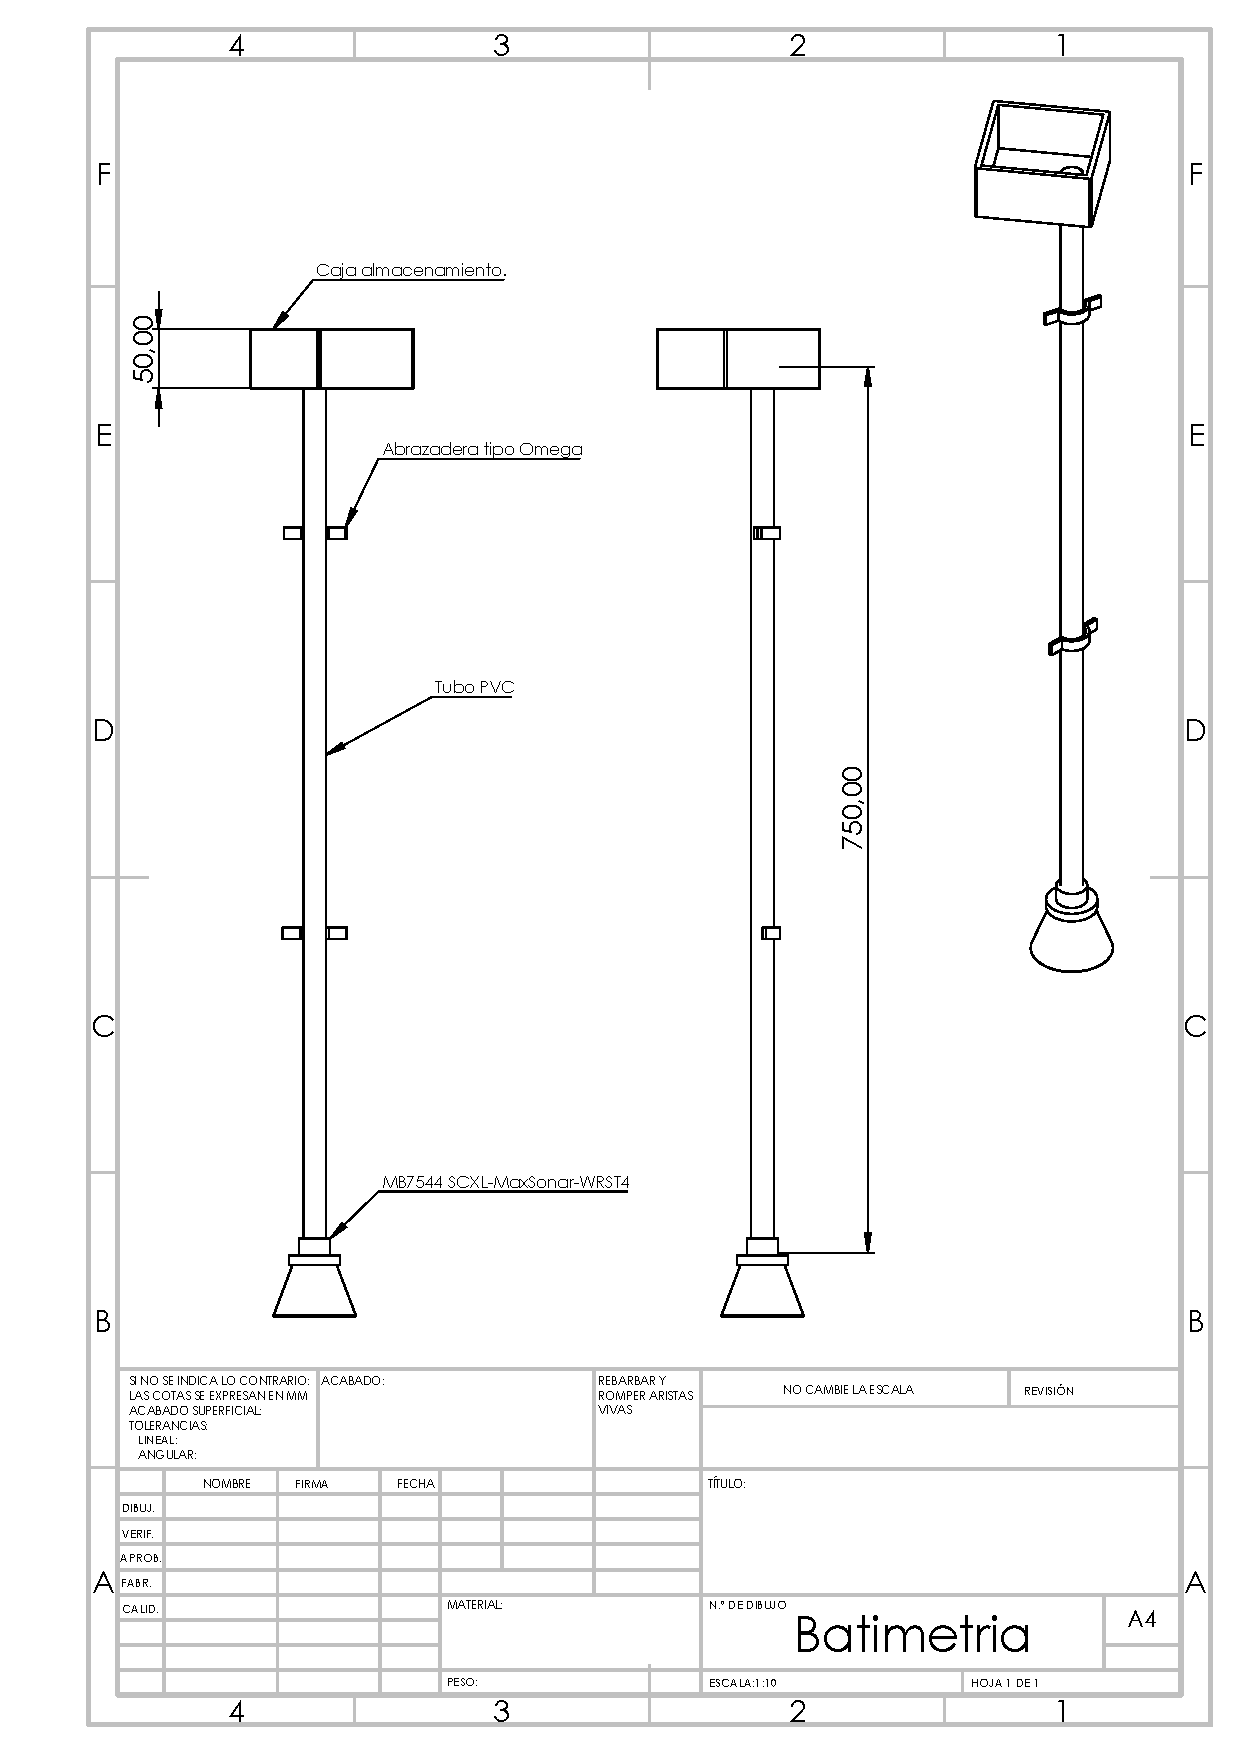
\includegraphics[scale=0.6]{Imagenes/cap3/Batimetria.pdf}}
\caption{Dise\~no final de medidor de profundidad. \textbf{Fuente:} elaboración propia}
\label{fig:batimetro}
\end{figure}

para estructura del sistema de batimetr\'ia tubos de PVC (Policloruro de Vinilo) roscables para la construcci\'on de la estructura de soporte, la secci\'on m\'as larga tiene una longitud de 1,5 [m], con el objetivo de poder ajustar la distancia de medici\'on inicial y que el sonar ubicado en el extremo est\'e totalmente sumergido. El sistema de fijaci\'on y ajuste est\'a compuesta por dos abrazaderas, una del tipo omega utilizada como gu\'ia de desplazamiento y la otra de abrazadora tipo "O" para el ajuste de profundidad. 


\subsubsection[Gr\'ua ]{Gr\'ua}





     \chapter[Pruebas y resultados experimentales]{ Pruebas y resultados experimentales}
\pagestyle{fancy}

En este cap\'itulo se abordar\'a los resultados obtenidos a fin de dar cumplimiento de los objetivos definidos en este TFG, adem\'as de verificación del correcto funcionamiento del sistema dise\~nado, mediantes los reportes y an\'alisis de datos obtenidos a partir de las  pruebas de funcionamiento en ambientes controlados y pruebas de campo en el Lago Ypakarai.  As\'i mismo  las configuraciones correspondientes a fin de obtener las lecturas en tiempo real en la estaci\'on remota, ubicada en la sala de monitoreo del laboratorio de sistemas. distribuido (LSD) en CITEC.
\section{Prueba en ambientes controlados}
Las pruebas en ambientes controlados, consisti\'o en una serie de pruebas realizados en el laboratorio de sistemas distribuido y en el laboratorio de qu\'imica, a fin de poner a punto todos los elementos que conforman el sistema a ser desplegados, antes de realizar las pruebas en campo, donde se espera que se encuentren m\'as variables a tener en cuenta, que deben prever y probar con anticipaci\'on de tal forma de evitar menos fallas.
En este efecto, en este apartado se abarcar\'an los trabajos realizados para la puesta a punto de los sensores Atlas Scientific.

\subsection{Calibraciones de sensores}
La calibraci\'on de los sensores, es fundamental para que pueda representar una lectura correcta de los valores a ser medidos, a este efecto los sensores adquiridos para la sonda, fueron prove\'idos en un kit que se puede observar en la figura \ref{fig:kit}, los cuales inclu\'ian l\'iquidos de calibraci\'on para cada uno de los sensores adquiridos. 

El kit de l\'iquidos de calibraciones est\'a compuesta un total de ocho botellas, de las cuales una de ellas contiene un l\'iquido de almacenamiento. Cada sensor posee un tipo de calibraci\'on distinta, que var\'ia seg\'un la cantidad de puntos que requiere para ajustar la curva de lectura de mediciones.
El caso del sensor de pH requiere de tres puntos de calibración (bajo, medio y alto), para los cuales se utiliza pH=4 para la calibraci\'on del punto bajo, pH=7 para la calibraci\'on del punto medio y pH=10 para la calibraci\'on del punto alto, con estas 3 calibraciones el sensor de pH se encuentra listo.
El sensor de OD, requiere dos puntos de calibraci\'on, la primera calibraci\'on que consiste en la calibraci\'on a los niveles de ox\'igeno atmosf\'erico y el segundo con su l\'iquido test correspondiente.
El sensor de OPR, solo requiere un valor conocido de OPR para su calibraci\'on, para su efecto se utiliza el l\'iquido de calibraci\'on que posee un valor de 225 mV.
El sensor de conductividad el\'ectrica, requiere de dos puntos de calibraci\'on (alto y bajo), para los cuales se utilizaron CE=12.880 $\mu S/cm$ para la calibraci\'on del punto bajo y CE=80.000 $\mu S/cm$ para la calibraci\'on del punto alto.

La calibraci\'on se realiza, con la sobrescritura del valor de lectura muestreado al l\'iquido de calibraci\'on, con el valor esperado seg\'un los datos proporcionados, mediante protocolo de comunicaci\'on i2C o serial, a la placa driver del sensor, con el comando \textbf{CAL,n }, donde CAL es el comando de calibraci\'on y n el valor a ser sobrescrito.
\begin{figure}[H]
        \centering
        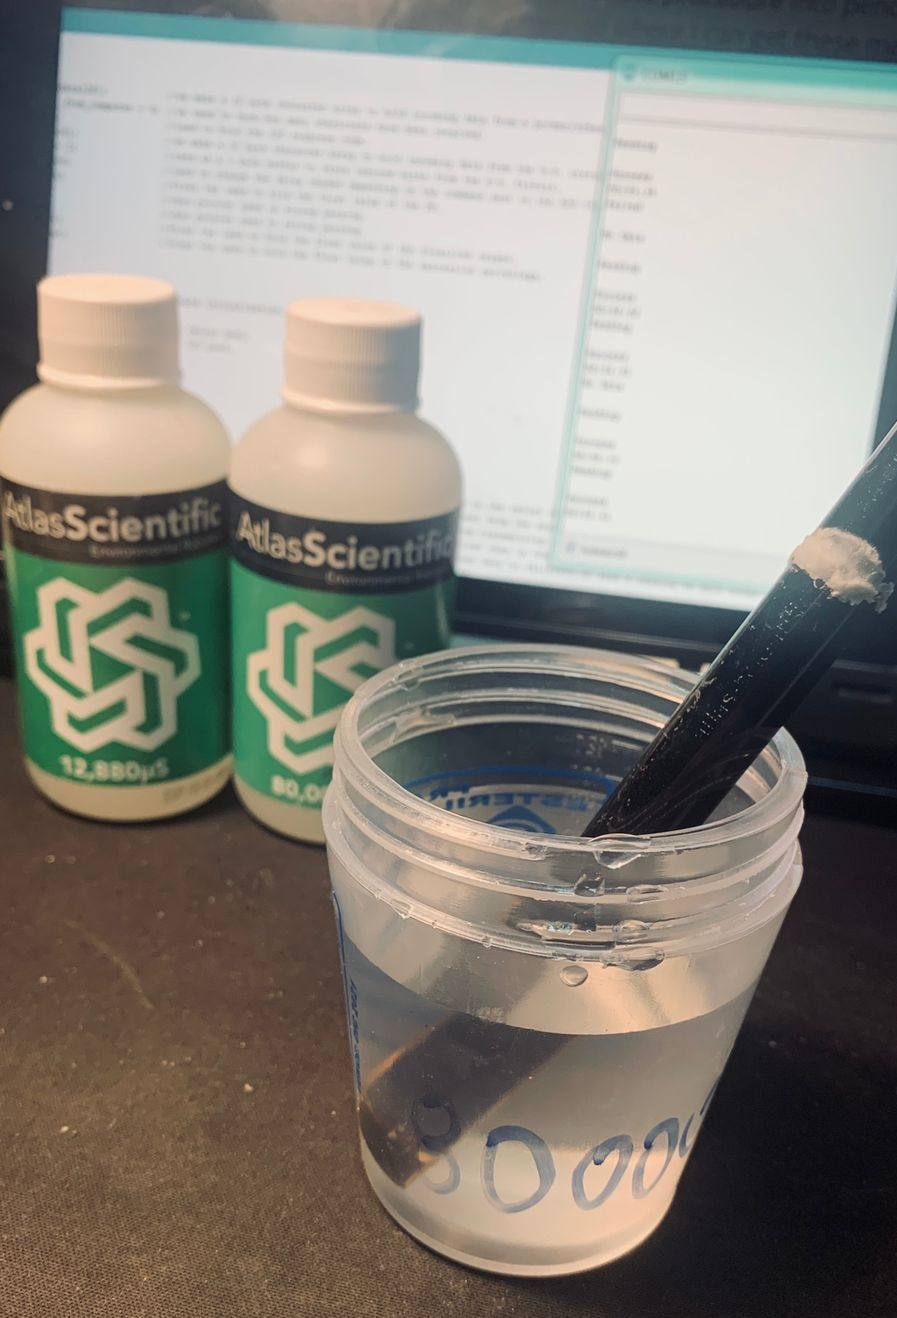
\includegraphics[scale=0.5]{Imagenes/cap4/calibracion.jpeg}
        \caption {Calibraci\'on sensor CE. }{\textbf{Fuente:}
        Elaboraci\'on propia}
        \label{fig:kit}
\end{figure}
Los sensores se consideran calibrados, si pueden realizar lecturas sobre l\'iquidos cuyos valores sean conocidos con un dentro del error esperado o previsto por el fabricante, en el caso de no conseguir una lectura correcta, se debe de borrar las configuraciones de calibraci\'on con el comando \textbf{Cal, clear} y volver a realizar el procedimiento anterior, una vez limpiado todos los equipos utilizados a fin de equipar contaminación. 
En el caso de los sensores de pH y OPR, se deben almacenar con su l\'iquido de almacenamiento.
\subsection{Muestreo en el laboratorio qu\'imica - FIUNA }
El monitoreo se realiz\'o en el laboratorio de qu\'imica de la facultad de ingenier\'ia de la Universidad Nacional de Asunci\'on [QCA], sede San Lorenzo, de los par\'ametros temperatura[T], conductividad el\'ectrica[CE], potencial de hidr\'ogeno[pH]. A fin de poder contrastar los sensores utilizados con los sensores disponibles en el laboratorio de qu\'imica.


\subsubsection{Metodolog\'ia }
La metodolog\'ia de recolección y muestreo consisti\'o en el an\'alisis de tres tipos de muestras distintas, la muestra 1 consisti\'o en agua doble destilada, la muestra 2 consisti\'o en agua de pozo, obtenida de una de las redes de abastecimiento de la zona del campus universitario y la muestra 3 consisti\'o en agua de laguna obtenida en la Facultad de Ciencias Exactas y Naturales (FACEN). Cada una de estas muestras se dividieron equitativamente en tres recipientes distintos, de tal forma de obtener el mismo l\'iquido en tres recientes que ser\'an muestreado y registrado las primeras 5 lecturas estables con el multisensor del laboratorio de qu\'imica e igual n\'umero de veces con los sensores de la sonda disen\~nada.
Los par\'ametros a ser analizados en este apartado son pH, CE y T, por la disponibilidad en ese momento de los equipos.
Las caracter\'isticas de los sensores del laboratorio de qu\'imica utilizados se pueden visualizar en la tabla \ref{tab: Sensores laboratorio de quimica}
Sensores laboratorio de qu\'imica, las caracter\'isticas de los otros sensores se encuentran en el cap\'itulo 2, correspondientes al sensor de CE,T,Ph de la empresa Atlas Scientific.
\begin{table}[H]
    \caption{Caracter\'isticas de los sensores de laboratorio de qu\'imica}
    \label{tab: Sensores laboratorio de quimica}
    \begin{tabular}{l c c}
        \toprule
        Caracter\'isticas & Sensor $pH$ & Sensor  $CE$ \\
        \midrule
        Marca & Ohaus       & Oaklon       \\
        Serie & ST10        & WD-35462-11  \\
        Intervalo de medici\'on                      & 0.00 – 14 {[}pH{]} & 0.00 – 20.00 {[}mS/cm{]}        \\
        Resoluci\'on de la medici\'on & 0.1   {[}pH{]}     & TDS 10 {[}ppm{]}, 0,1 {[}ppt{]} \\
        Precisi\'on                                  & $\pm0,1$ {[}pH{]}  & $\pm0,1$ {[}mS/cm{]}   
    \end{tabular}
 \end{table}
Las lecturas se realizaron de forma secuencial con ambos sensores, figura \ref{fig: Muestreo de CE}, cada vez que terminaba el muestreo en cada uno de el recipiente con una de la muestras, se proced\'ia registrar la lectura estable obtenida, retirar el sensor utilizado, limpiarlo con agua destilada y secar con un pa\~no, e introducir el otro sensor equivalente para repetir el procedimiento hasta completar los cinco muestreos.

\begin{figure}
     \centering
     \begin{subfigure}[b]{0.25\textwidth}
         \centering
         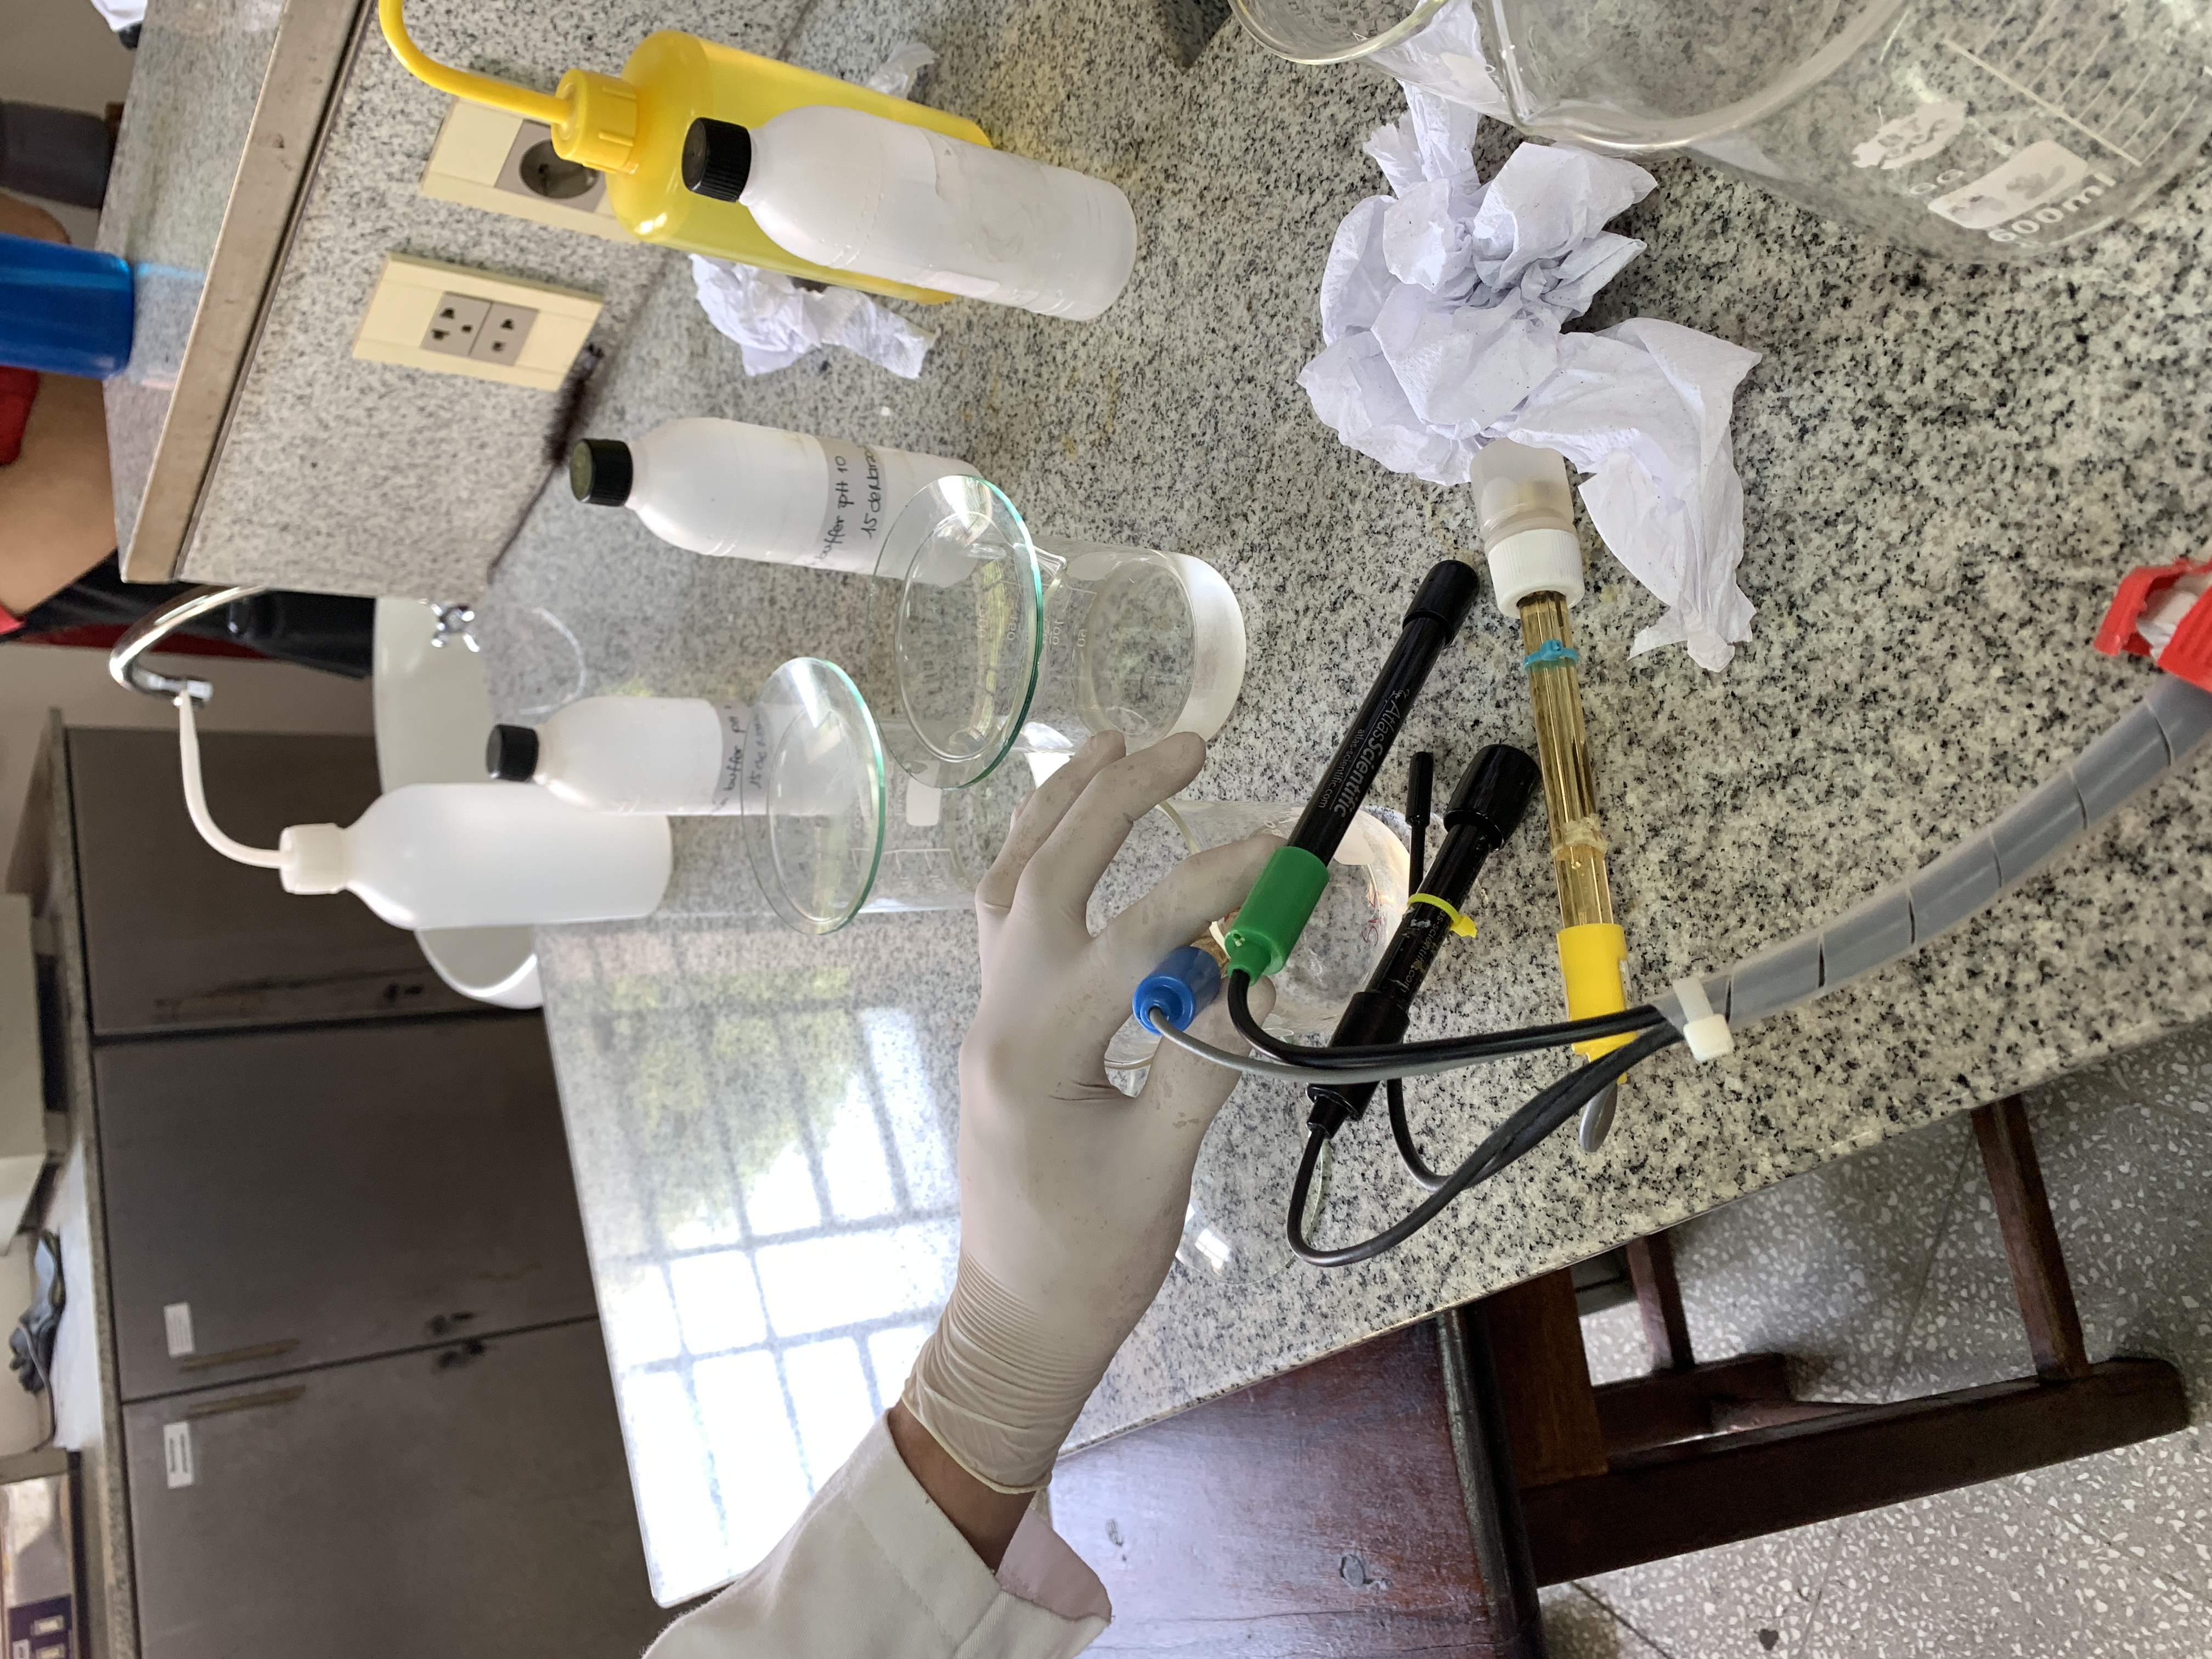
\includegraphics[angle=270,width=\textwidth]{Imagenes/cap4/qca1.jpg}
         \caption{Sensores sonda.}
         \label{fig:calibracionLSD}
     \end{subfigure}
     \hfill
     \begin{subfigure}[b]{0.4\textwidth}
         \centering
         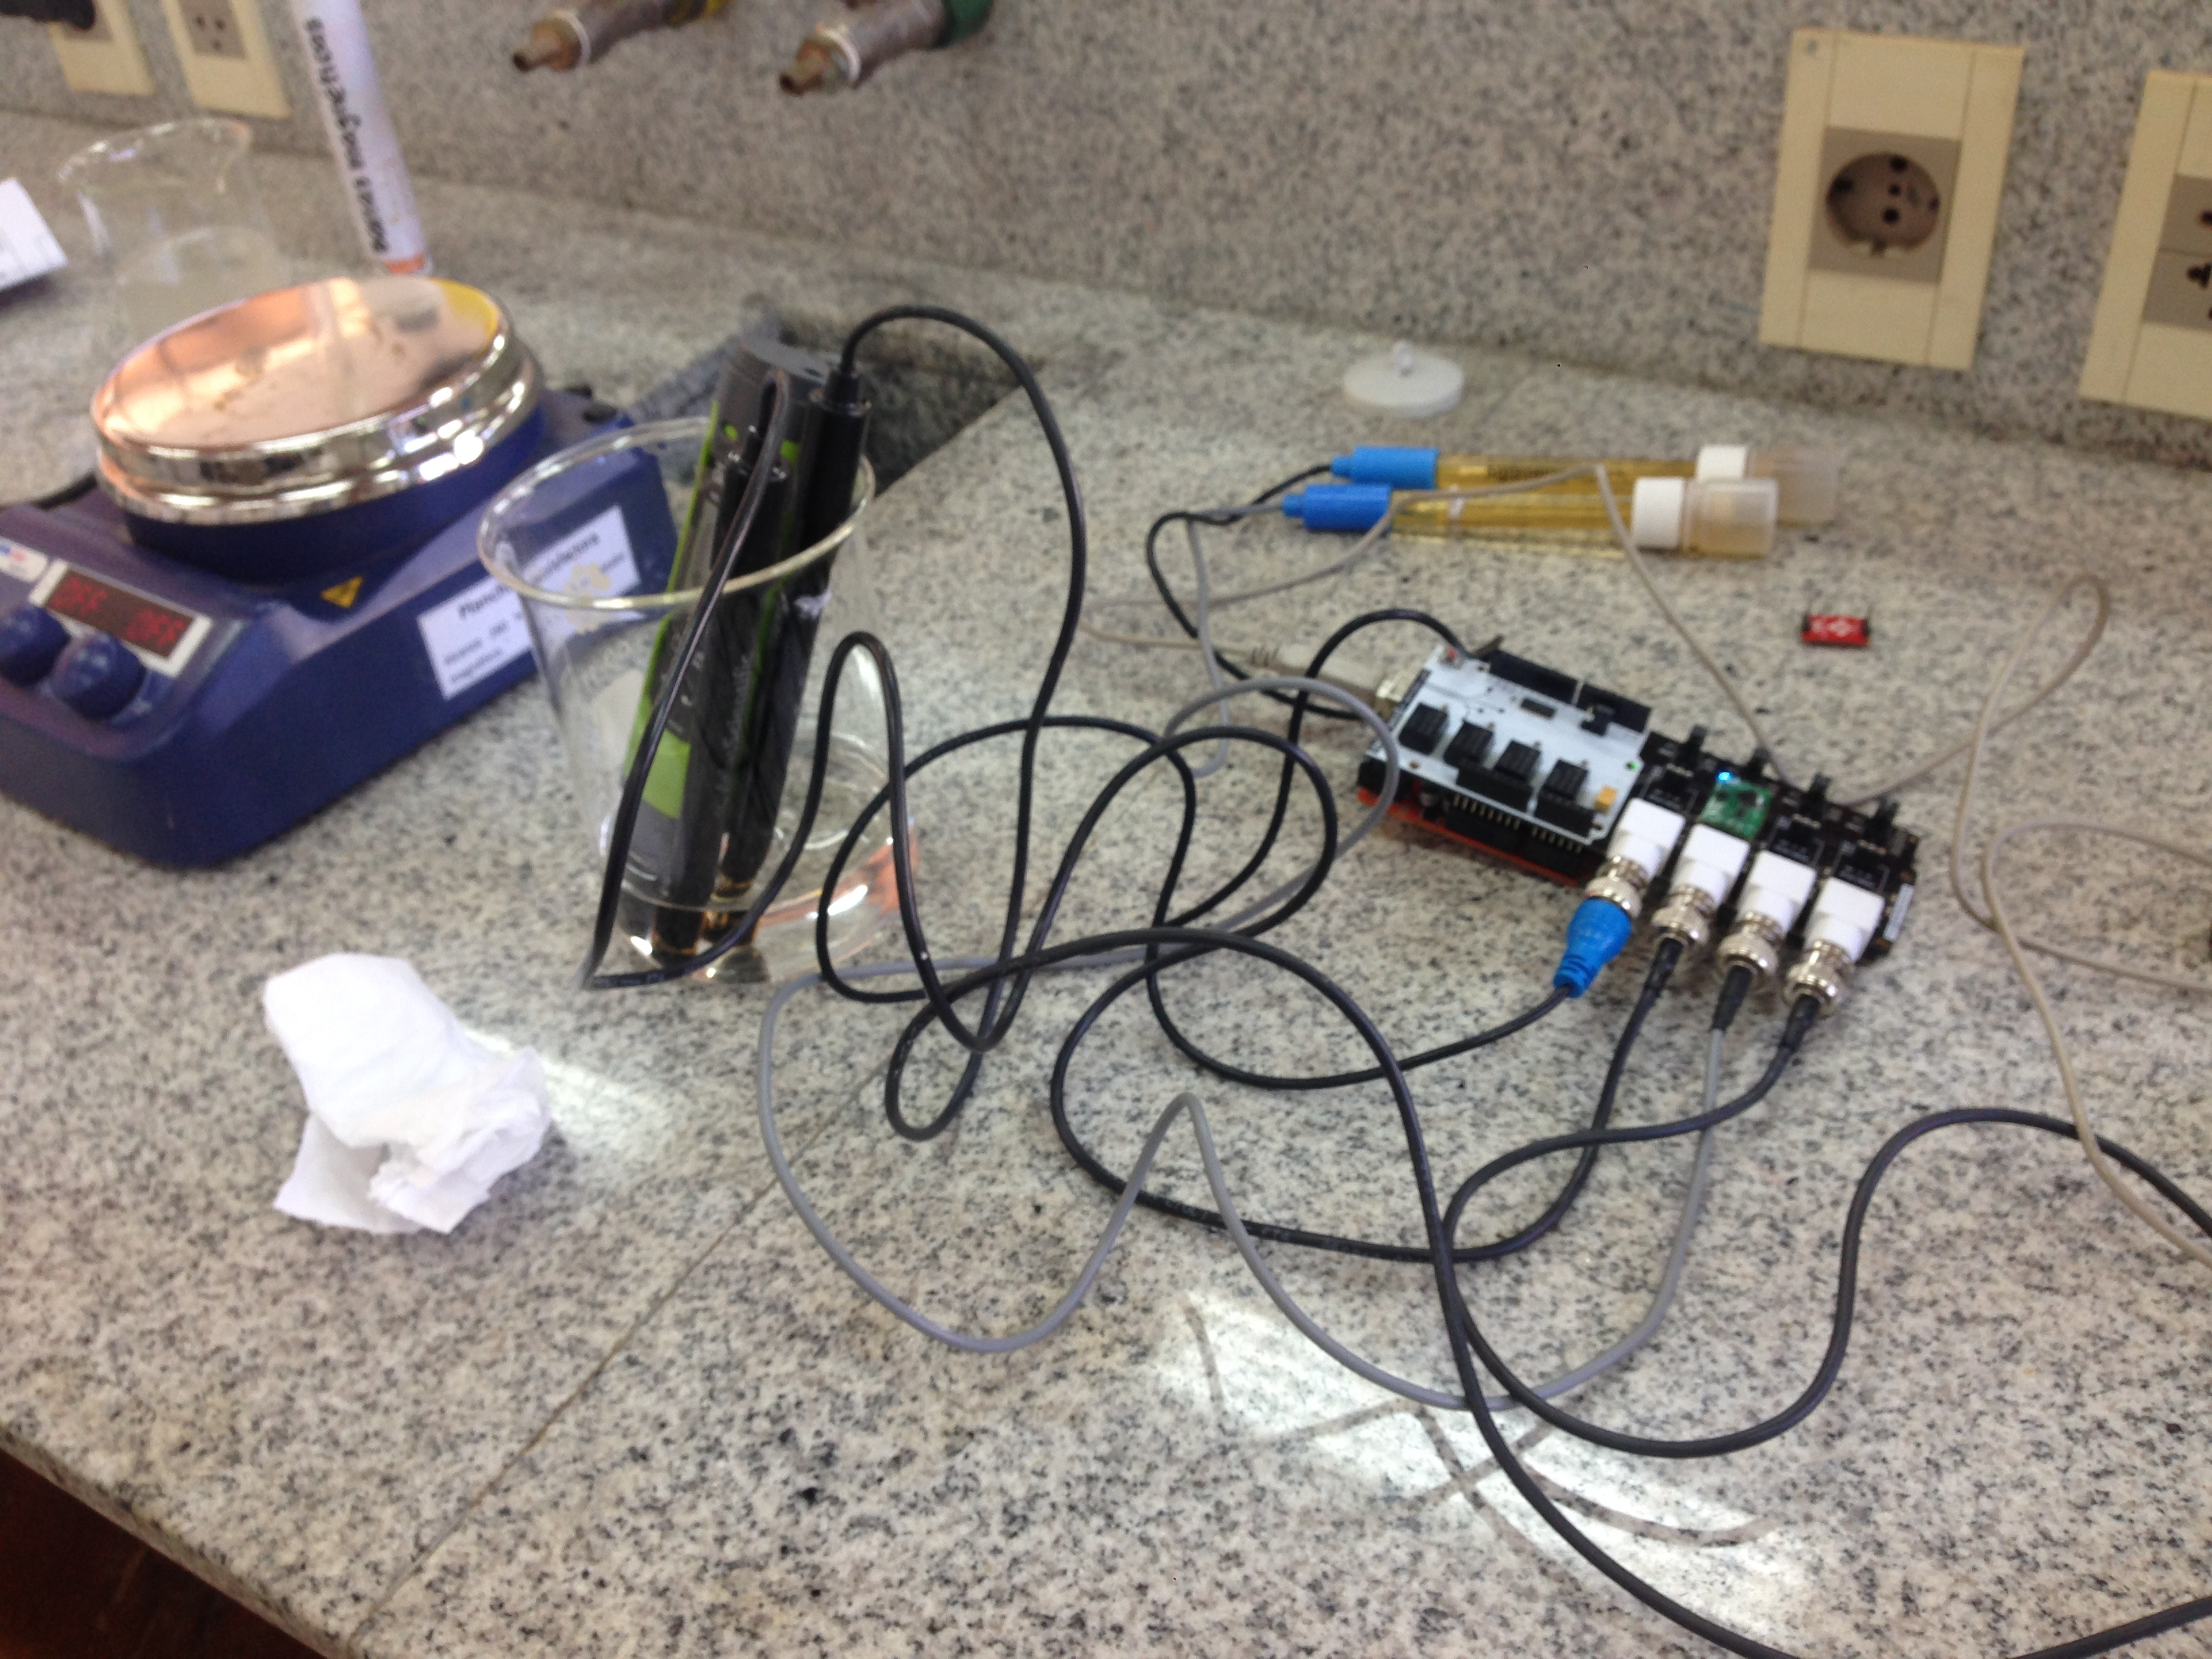
\includegraphics[width=\textwidth]{Imagenes/cap4/qca2.jpg}
         \caption{Placa de sensores}
         \label{fig:placas_muestreo}
     \end{subfigure}
     \hfill
     \begin{subfigure}[b]{0.25\textwidth}
         \centering
         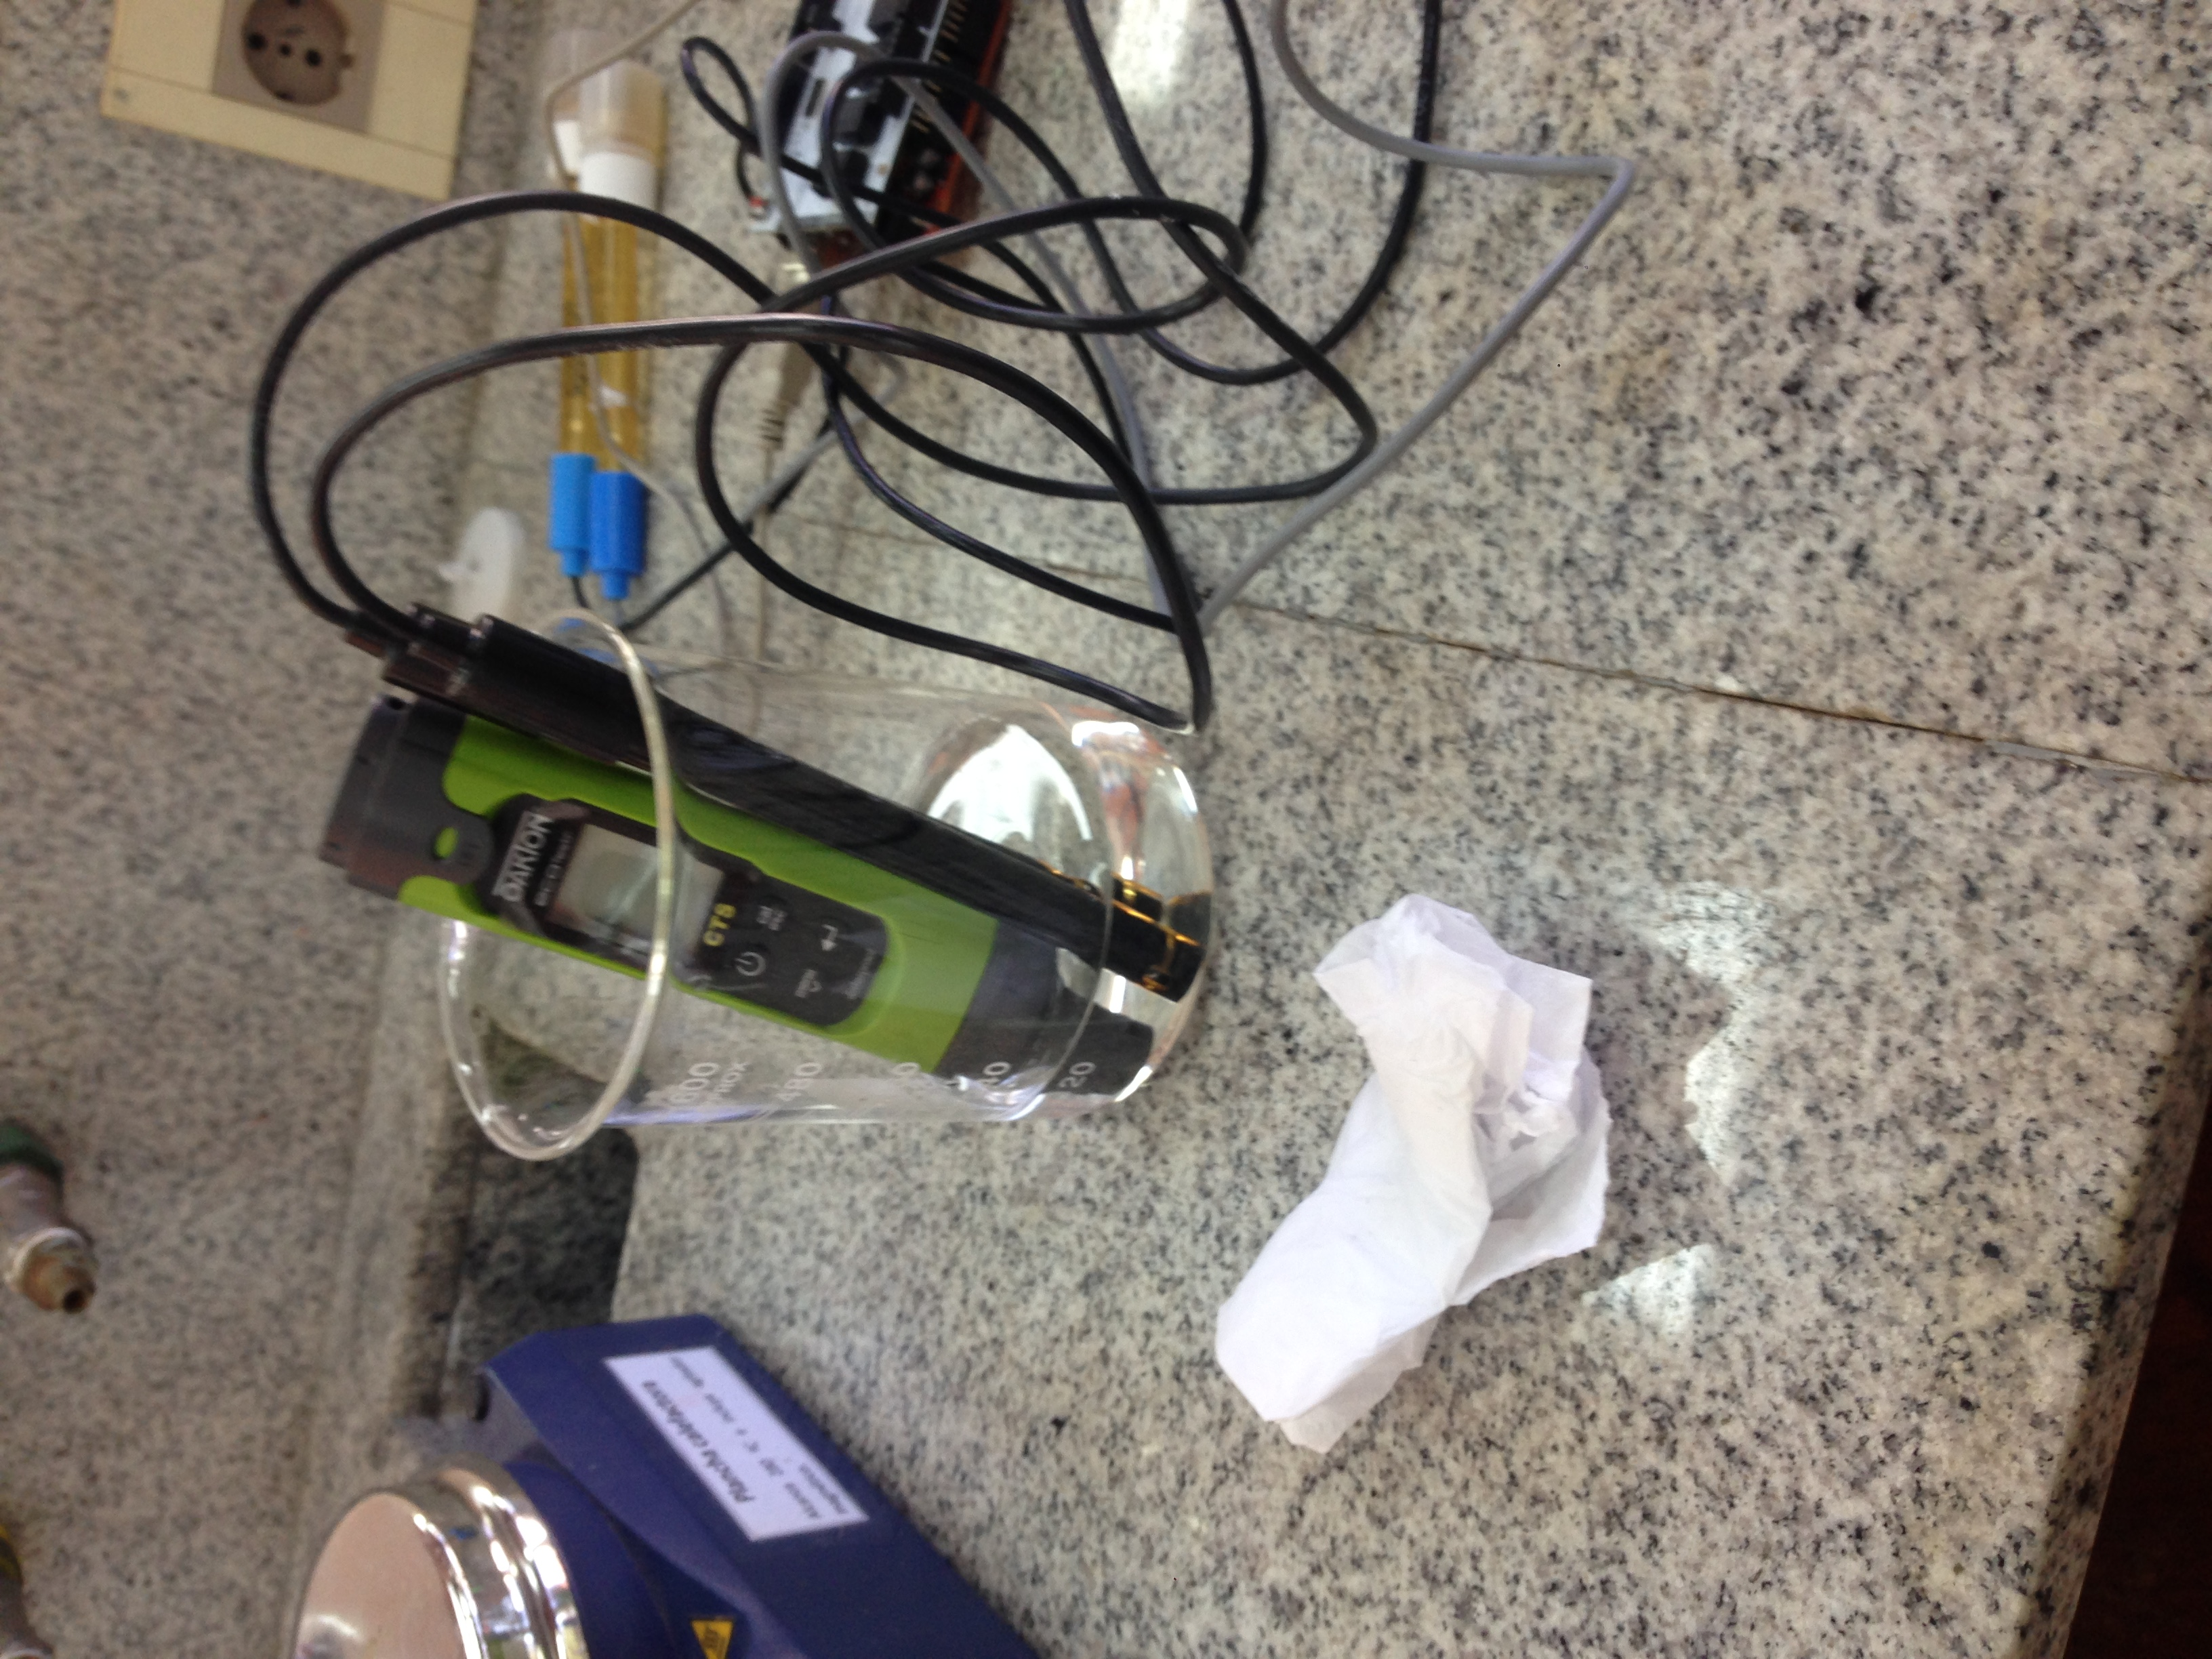
\includegraphics[angle=270,width=\textwidth]{Imagenes/cap4/qca3.jpg}
         \caption{Muestreo de CE}
         \label{fig: Muestreo de CE}
     \end{subfigure}
        \caption{Muestreo en el laboratorio qu\'imica - FIUNA}
        \label{fig:muestreoQCA}
\end{figure}


\newpage
\subsubsection{Muestra 1. Sensor de temperatura}
    \begin{table}[H]
        \protect\caption[Muestra 1: Destilada ]{Muestra 1: Agua de destilada.}
        \label{tab:TMuestra1}
        \centering
        \begin{tabular}{c c c}
            \hline
            \multicolumn{3}{c}{\textbf{Muestra 1: Agua de destilada}} \\
             \hline
            \multicolumn{3}{c}{\textbf{Recipiente 1}} \\
            \hline
            \textbf{Lectura}&\textbf{LSD ($^{\circ}$C)}&\textbf{Qca ($^{\circ}$C)} \\
            \hline
            {1}& $25.7$&$25.5$ \\ 
            % \hline
            {2}& $25.4$&$25.5$ \\ 
            % \hline
             {3}& $25.6$&$25.6$\\  
            % \hline
            {4}& $25.4$&$25.5$\\ 
            % \hline
            {5}& $25.2$&$25.6$ \\
            \hline
                       \multicolumn{3}{c}{\textbf{Recipiente 2}} \\
            \hline
            \textbf{Lectura}&\textbf{LSD ($^{\circ}$C)}&\textbf{Qca ($^{\circ}$C)} \\
            \hline
            {1}& $25.5$&$25.3$ \\ 
            % \hline
            {2}& $25.4$&$25.3$ \\ 
            % \hline
             {3}& $25.2$&$25.3$\\  
            % \hline
            {4}& $24.8$&$25.4$\\ 
            % \hline
            {5}& $24.6$&$25.4$ \\ 
            \hline
            \multicolumn{3}{c}{\textbf{Recipiente 3}} \\
            \hline
            \textbf{Lectura}&\textbf{LSD ($^{\circ}$C)}&\textbf{Qca´($^{\circ}$C)} \\
            \hline
            {1}& $24.6$&$25.4$ \\ 
            % \hline
            {2}& $25.6$&$25.6$ \\ 
            % \hline
             {3}& $25.9$&$25.6$\\  
            % \hline
            {4}& $25.6$&$25.4$\\ 
            % \hline
            {5}& $25.4$&$25.3$ \\ 
            \hline
        \end{tabular}
        \vspace{5mm}
        \newline
        \hfill \textbf{Fuente: }Elaboración Propia.
    \end{table}

% Grafico M1T
\begin{figure}[H]
        \centering
        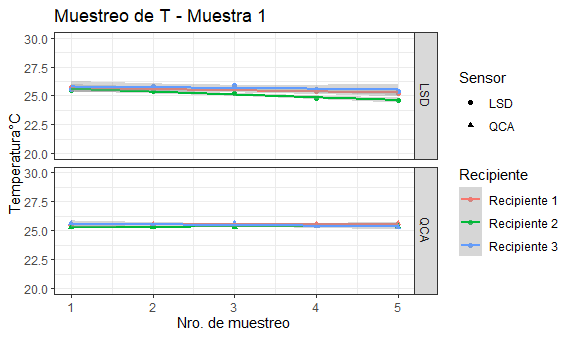
\includegraphics[width=0.75\linewidth]{Imagenes/cap4/T_M1.png}
        \caption {Muestreo de temperatura. }{\textbf{Fuente:}
        Elaboraci\'on Propia. }
        \label{fig:M1T}
    \end{figure}
    
\subsubsection{Muestra 1. Sensor Conductividad El\'ectrica}
    \begin{table}[H]
        \protect\caption[Muestra 1: Destilada ]{Muestra 1: Agua de destilada.}
        \label{tab:TMuestra1}
        \centering
        \begin{tabular}{c c c}
            \hline
            \multicolumn{3}{c}{\textbf{Muestra 1: Agua de destilada}} \\
             \hline
            \multicolumn{3}{c}{\textbf{Recipiente 1}} \\
            \hline
            \textbf{Lectura}&\textbf{LSD ($\mu S/cm$)}&\textbf{Qca ($\mu S/cm$)} \\
            \hline
            {1}& $0$&$0$ \\ 
            % \hline
            {2}& $0$&$0$ \\ 
            % \hline
             {3}& $0$&$0$\\  
            % \hline
            {4}& $0$&$0$\\ 
            % \hline
            {5}& $0$&$0$ \\
            \hline
                       \multicolumn{3}{c}{\textbf{Recipiente 2}} \\
            \hline
            \textbf{Lectura}&\textbf{LSD ($\mu S/cm$)}&\textbf{Qca ($\mu S/cm$)} \\
            \hline
            {1}& $0$&$0$ \\ 
            % \hline
            {2}& $0$&$0$ \\ 
            % \hline
            {3}& $0$&$0$\\  
            % \hline
            {4}& $0$&$0$\\ 
            % \hline
            {5}& $0$&$0$ \\
            \hline
            \multicolumn{3}{c}{\textbf{Recipiente 3}} \\
            \hline
            \textbf{Lectura}&\textbf{LSD ($\mu S/cm$)}&\textbf{Qca ($\mu S/cm$)} \\
            \hline
            {1}& $0$&$0$ \\ 
            % \hline
            {2}& $0$&$0$ \\ 
            % \hline
             {3}& $0$&$0$\\  
            % \hline
            {4}& $0$&$0$\\ 
            % \hline
            {5}& $0$&$0$ \\
            \hline
        \end{tabular}
        \vspace{5mm}
        \newline
        \hfill \textbf{Fuente: }Elaboración Propia.
    \end{table}

% Grafico M1CE
    \begin{figure}[H]
        \centering
        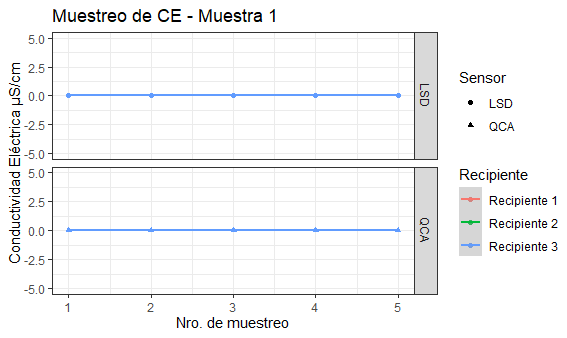
\includegraphics[width=0.75\linewidth]{Imagenes/cap4/CE_M1.png}
        \caption {Muestreo de conductividad el\'ectrica. }{\textbf{Fuente:}
        Elaboraci\'on Propia. }
        \label{fig:M1CE}
    \end{figure}

\subsubsection{Muestra 1. Sensor de pH}
    \begin{table}[H]
        \protect\caption[Muestra 1: Destilada ]{Muestra 1: Agua de destilada.}
        \label{tab:TMuestra1}
        \centering
        \begin{tabular}{c c c}
            \hline
            \multicolumn{3}{c}{\textbf{Muestra 1: Agua de destilada}} \\
             \hline
            \multicolumn{3}{c}{\textbf{Recipiente 1}} \\
            \hline
            \textbf{Lectura}&\textbf{LSD ($pH$)}&\textbf{Qca ($pH$)} \\
            \hline
            {1}& $6.898$&$8.27$ \\ 
            % \hline
            {2}& $6.853$&$7.86$ \\ 
            % \hline
            {3}& $6.856$&$7.36$\\  
            % \hline
            {4}& $6.809$&$6.82$\\ 
            % \hline
            {5}& $6.715$&$6.86$ \\
            \hline
            \multicolumn{3}{c}{\textbf{Recipiente 2}} \\
            \hline
            \textbf{Lectura}&\textbf{LSD ($pH$)}&\textbf{Qca ($pH$)} \\
            \hline
            {1}& $6.555$&$6.59$ \\ 
            % \hline
            {2}& $6.303$&$6.88$ \\ 
            % \hline
            {3}& $5.919$&$6.76$\\  
            % \hline
            {4}& $5.502$&$6.65$\\ 
            % \hline
            {5}& $5.171$&$6.62$ \\
            \hline
            \multicolumn{3}{c}{\textbf{Recipiente 3}} \\
            \hline
            \textbf{Lectura}&\textbf{LSD ($pH$)}&\textbf{Qca ($pH$)} \\
            \hline
            {1}& $6.495$&$6.86$ \\ 
            % \hline
            {2}& $6.440$&$6.77$ \\ 
            % \hline
             {3}& $6.316$&$6.49$\\  
            % \hline
            {4}& $6.711$&$6.18$\\ 
            % \hline
            {5}& $6.613$&$6.37$ \\
            \hline
        \end{tabular}
        \vspace{5mm}
        \newline
        \hfill \textbf{Fuente: }Elaboración Propia.
    \end{table}

% Grafico M1Ph
    \begin{figure}[H]
        \centering
        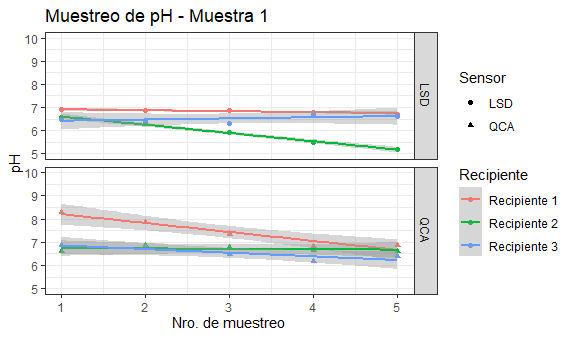
\includegraphics[width=0.75\linewidth]{Imagenes/cap4/pH_M1.png}
        \caption {Muestreo de pH. }{\textbf{Fuente:}
        Elaboraci\'on Propia. }
        \label{fig:M1PH}
    \end{figure}

\subsubsection{An\'alisis de Datos. Muestra 1}
% Please add the following required packages to your document preamble:

\begin{table}[H]
\protect\caption[Muestra 1: Destilada ]{Estad\'isticas de mediciones: Muestra 1.}
\label{tab:AnalisisM1}
\begin{tabular}{l ccc|ccc}
\hline
\textbf{Muestra 1  }& \multicolumn{3}{c}{LSD} & \multicolumn{3}{c}{QCA}  \\ 
\begin{tabular}[c]{@{}l@{}}An\'alisis de datos\end{tabular} & \multicolumn{1}{c}{\begin{tabular}[c]{@{}c@{}}T \\$ ^{\circ}C$\end{tabular}} & \multicolumn{1}{c}{pH}        & \begin{tabular}[c]{@{}c@{}}CE\\ $\mu S/cm$\end{tabular} & \multicolumn{1}{c}{\begin{tabular}[c]{@{}c@{}}T \\$ ^{\circ}C$\end{tabular}} & \multicolumn{1}{c}{pH}        & \multicolumn{1}{c}{\begin{tabular}[c]{@{}c@{}}CE\\ $\mu S/cm$\end{tabular}} \\ 
\hline
Desviaci\'on Est\'andar & \multicolumn{1}{c}{0.349} & \multicolumn{1}{c}{0.511} & 0                                                  & \multicolumn{1}{c}{0.118}                                       & \multicolumn{1}{c}{0.551} & \multicolumn{1}{c}{0}                                                  \\ 
Varianza                                                                        & \multicolumn{1}{c}{0.122}                                       & \multicolumn{1}{c}{0.261} & 0                                                  & \multicolumn{1}{c}{0.014}                                      & \multicolumn{1}{c}{0.304} & \multicolumn{1}{c}{0}                                                  \\ 
Error Estándar                                                                  & \multicolumn{1}{c}{0.090}                                      & \multicolumn{1}{c}{0.132} & 0                                                  & \multicolumn{1}{c}{0.0306}                                      & \multicolumn{1}{c}{0.142} & \multicolumn{1}{c}{0}                                                  \\ 
Mínimo  &   \multicolumn{1}{c}{24.60}  & \multicolumn{1}{r}{5.171} & 0 & \multicolumn{1}{c}{25.30} & \multicolumn{1}{r}{6.180} & 0 \\
% \hline
Máximo  & \multicolumn{1}{c}{25.90}    & \multicolumn{1}{c}{6.898} & 0 & \multicolumn{1}{c}{25.60}  & \multicolumn{1}{c}{8.270} & 0  \\ 
% \hline
Promedio & \multicolumn{1}{c}{25.41}   & \multicolumn{1}{c}{6.410} & 0 & \multicolumn{1}{c}{25.45} & \multicolumn{1}{c}{6.889} & 0 
\\ 
\hline
\end{tabular}
\vspace{5mm}
\newline
\hfill \textbf{Fuente: }Elaboración Propia.
\end{table}

En la tabla \ref{tab:AnalisisM1}, se puede observar algunos par\'metros estad\'isticos calculados, a partir de los registros recolectados en el muestreo de los recipientes de la muestra 1, el cual arrojo los siguientes resultados. La desviaci\'on est\'andar en el caso de la temperatura, presenta en ambos caso un \'indice bajo m\'as aun para el equipo de QCA, por lo cual indica que la mayor parte de los datos de una muestra tienden a estar agrupados cerca de su media. En caso del pH la desviaci\'on est\'andar es un poco mayor, pero de igual manera baja, por lo tanto, tambi\'en tienen tendencia que las lecturas se agrupen cerca de la media. La varianza sigue la misma tendencia de la desviaci\'on est\'andar, por lo tanto, todos los datos recolectados no presentan dispersi\'on. El error est\'andar, presenta valores bajos en todo los par\'ametros, el cual sugiere que los valores recolectados son uniforme y se encuentran cerca de la media. Los valores mínimos recolectados en el caso de la temperatura presentan una deferencia de 0,7 $ ^{\circ}C$ siendo 25.3 $ ^{\circ}C$ la menor lectura registrada por el sensor de QCA, en el caso del pH la diferencia entre los mínimos fue de 1.009 pH, siendo 5.171 pH la menor lectura registrada por el sensor de LSD. Los valores m\'aximo recolectados en el caso de la temperatura presentan una deferencia de 0,3 $ ^{\circ}C$ siendo 25.90 $ ^{\circ}C$ la mayor lectura registrada por el sensor de LSD, en el caso del pH la diferencia entre los m\'aximos fue de 1.372 pH, siendo 8.270 pH la mayor lectura registrada por el sensor de QCA. El promedio de las mediciones fueron cercanas con una diferencia de 7$\%$ en el caso del pH, siendo el promedio de los datos de pH registrado por el sensor de QCA 6.889 pH contra el promedio de pH registrado por el sensor LSD igual a 6.41 pH, en el caso de los resultados promedios registrados de la temperatura la diferencia entre los resultados fue menor al 0.5$\%$ siendo la temperatura promedio del sensor LSD igual a 24.41$ ^{\circ}C$ y la temperatura promedio del sensor de QCA igual a 25.25$^{\circ}C$. En este an\'alisis de datos correspondiente a la muestra 1, no sé describi\'o los datos recolectados por el sensor de CE, ya que en ambos sensores se obtuvieron los mismos resultados iguales a 0 $\mu S/cm$, tal como se espera para este tipo de muestra.

\begin{table}[]
\caption{Relaci\'on entre los equipos de sensores}
\label{tab:VaCoM1}
\centering
\begin{tabular}{llll} 
\toprule
& T   &  pH    & CE \\
\midrule
Covarianza  & 0.0125& 0.111 & 0                \\
Correlación & 0.301& 0.395 & 0        \\
\bottomrule
\end{tabular}
\\ \textbf{Fuente: }Elaboración Propia.
\end{table}     
% https://sitiobigdata.com/2019/10/26/covarianza-y-correlacion/


En la tabla \ref{tab:VaCoM1}, se analizan los resultados de covarianza y correlación de las muestras, en el caso de la temperatura y pH se obtuvieron unas covarianzas positivas el cual indica que ambas lecturas varían en la misma dirección, as\'i mismo en ambos par\'ametros se obtuvieron correlaciones positivas lo cual indica que son directamente proporcionales entre sí, la media varía en la misma dirección con el factor del valor del coeficiente de correlación. Luego de analizar los resultados obtenidos en el caso de la muestra 1, se puede concluir que ambos sensores presentan lecturas cercanas, con baja dispersi\'on. 

%% Muestra nro 2: Agua de Pozo
\subsubsection{Muestra 2.Temperatura}
    \begin{table}[H]
        \protect\caption[Muestra 2: Agua de pozo ]{Muestra 2: Agua de pozo.}
        \label{tab:TMuestra2}
        \centering
        \begin{tabular}{c c c}
            \hline
            \multicolumn{3}{c}{\textbf{Muestra 2: Agua de pozo.}} \\
             \hline
            \multicolumn{3}{c}{\textbf{Recipiente 1}} \\
            \hline
            \textbf{Lectura}&\textbf{LSD($^{\circ}$C)}&\textbf{Qca($^{\circ}$C)} \\
            \hline
            {1}& $23.6$&$25.1$ \\ 
            % \hline
            {2}& $22.9$&$24.9$ \\ 
            % \hline
             {3}& $22.6$&$24.8$\\  
            % \hline
            {4}& $22.5$&$24.6$\\ 
            % \hline
            {5}& $22.3$&$24.6$ \\
            \hline
                       \multicolumn{3}{c}{\textbf{Recipiente 2}} \\
            \hline
            \textbf{Lectura}&\textbf{LSD($^{\circ}$C)}&\textbf{Qca($^{\circ}$C)} \\
            \hline
            {1}& $24.4$&$24.4$ \\ 
            % \hline
            {2}& $24.0$&$24.2$ \\ 
            % \hline
             {3}& $23.9$&$24.0$\\  
            % \hline
            {4}& $23.9$&$23.9$\\ 
            % \hline
            {5}& $23.8$&$23.9$ \\ 
            \hline
            \multicolumn{3}{c}{\textbf{Recipiente 3}} \\
            \hline
            \textbf{Lectura}&\textbf{LSD($^{\circ}$C)}&\textbf{Qca($^{\circ}$C)} \\
            \hline
            {1}& $22.2$&$23.9$ \\ 
            % \hline
            {2}& $21.9$&$24.0$ \\ 
            % \hline
             {3}& $21.5$&$23.8$\\  
            % \hline
            {4}& $21.4$&$23.7$\\ 
            % \hline
            {5}& $21.2$&$23.6$ \\ 
            \hline
        \end{tabular}
        \vspace{5mm}
        \newline
        \hfill \textbf{Fuente: }Elaboración Propia.
    \end{table}

% Gráfico M2T
    \begin{figure}[H]
        \centering
        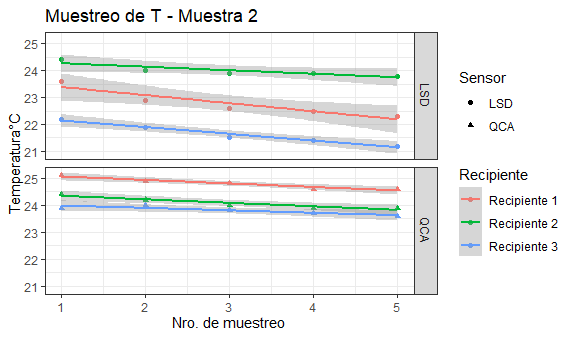
\includegraphics[width=0.75\linewidth]{Imagenes/cap4/T_M2.png}
        \caption {Muestreo de temperatura. }{\textbf{Fuente:}
        Elaboraci\'on Propia. }
        \label{fig:M2T}
    \end{figure}

\subsubsection{Muestra 2. Sensor Conductividad El\'ectrica }
    \begin{table}[H]
        \protect\caption[Muestra 2: Agua de pozo ]{Muestra 2: Agua de pozo.}
        \label{tab:CEMuestra2}
        \centering
        \begin{tabular}{c c c }
            \hline
            \multicolumn{3}{c}{\textbf{Muestra 2: Agua de pozo}} \\
             \hline
            \multicolumn{3}{c}{\textbf{Recipiente 1}} \\
            \hline
            \textbf{Lectura}&\textbf{LSD ($\mu S/cm$)}&\textbf{Qca ($\mu S/cm$)} \\
            \hline
            {1}& $81.39$&$100$ \\ 
            {2}& $80.12$&$90$ \\ 
            {3}&$80.05$&$90$\\  
            {4}& $80.55$&$100$\\ 
            {5}& $80.10$&$90$ \\
            \hline
                       \multicolumn{3}{c}{\textbf{Recipiente 2}} \\
            \hline
            \textbf{Lectura}&\textbf{LSD ($\mu S/cm$)}&\textbf{Qca ($\mu S/cm$)} \\
            \hline
            {1}& $80.32$&$80$ \\ 
            {2}& $80.36$&$80$ \\ 
            {3}&$80.40$&$80$  \\  
            {4}& $80.45$&$80$ \\ 
            {5}& $80.49$&$80$ \\ 
            \hline
            \multicolumn{3}{c}{\textbf{Recipiente 3}} \\
            \hline
            \textbf{Lectura}&\textbf{LSD ($\mu S/cm$)}&\textbf{Qca($\mu S/cm$)} \\
            \hline
            {1}& $119.60$&$130$ \\ 
            {2}& $110.30$&$130$ \\ 
            {3}&$118.90$&$130$  \\  
            {4}& $117.10$&$130$ \\ 
            {5}& $118.40$&$130$ \\ 
            \hline
        \end{tabular}
        \vspace{5mm}
        \newline
        \hfill \textbf{Fuente: }Elaboración Propia.
    \end{table}

% Gráfico M2CE
    \begin{figure}[H]
        \centering
        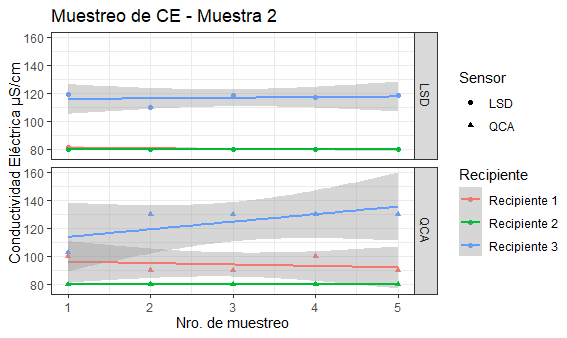
\includegraphics[width=0.75\linewidth]{Imagenes/cap4/CE_M2.png}
        \caption {Muestreo de conductividad el\'ectrica. }{\textbf{Fuente:}
        Elaboraci\'on Propia. }
        \label{fig:M2CE}
    \end{figure}

\subsubsection{Muestra 2. Sensor de pH}
    \begin{table}[H]
        \protect\caption[Muestra 2: Agua de pozo ]{Muestra 2: Agua de pozo.}
        \label{tab:phMuestra2}
        \centering
        \begin{tabular}{c c c}
            \hline
            \multicolumn{3}{c}{\textbf{Muestra 2: Agua de pozo.}} \\
             \hline
            \multicolumn{3}{c}{\textbf{Recipiente 1}} \\
            \hline
            \textbf{Lectura}&\textbf{LSD ($pH$)}&\textbf{Qca ($pH$)} \\
            \hline
            {1}& $5.569$&$6.12$ \\ 
            {2}& $5.513$&$6.15$ \\ 
            {3}& $5.458$&$6.13$\\  
            {4}& $5.402$&$6.17$\\ 
            {5}& $5.498$&$6.20$ \\
            \hline
            \multicolumn{3}{c}{\textbf{Recipiente 2}} \\
            \hline
            \textbf{Lectura}&\textbf{LSD ($pH$)}&\textbf{Qca ($pH$)} \\
            \hline
            {1}& $5.157$&$5.94$ \\ 
            {2}& $5.251$&$5.96$ \\ 
            {3}& $5.552$&$5.98$ \\  
            {4}& $5.595$&$6.03$ \\ 
            {5}& $5.551$&$6.01$ \\
            \hline
            \multicolumn{3}{c}{\textbf{Recipiente 3}} \\
            \hline
            \textbf{Lectura}&\textbf{LSD ($pH$)}&\textbf{Qca ($pH$)} \\
            \hline
            {1}& $5.582$&$5.91$ \\ 
            {2}& $5.624$&$6.04$ \\ 
            {3}&$5.732$&$6.11$ \\  
            {4}& $5.918$&$6.09$\\ 
            {5}& $5.936$&$6.18$ \\
            \hline
        \end{tabular}
        \vspace{5mm}
        \newline
        \hfill \textbf{Fuente: }Elaboración Propia.
    \end{table}

% Gráfico M2pH
    \begin{figure}[H]
        \centering
        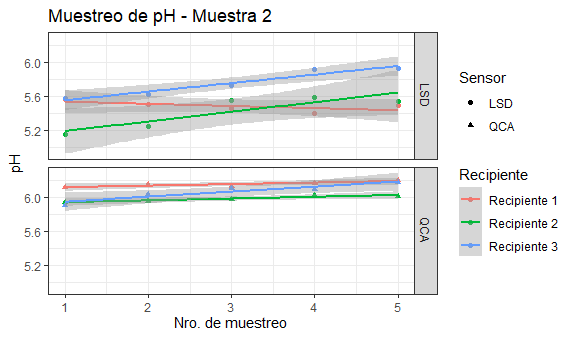
\includegraphics[width=0.75\linewidth]{Imagenes/cap4/pH_M2.png}
        \caption {Muestreo de pH. }{\textbf{Fuente:}
        Elaboraci\'on Propia. }
        \label{fig:M2PH}
    \end{figure}

\subsection{An\'alsis de Datos. Muestra 2}

\begin{table}[H]
    \protect\caption[Muestra 2: Agua de pozo ]{Resumen de mediciones: Muestra 2.}
\label{tab:AnalisisM2}

    \begin{tabular}{lccc|ccc}
    \hline
    Muestra 2 & 
    \multicolumn{3}{c}{LSD} & 
    \multicolumn{3}{c}{QCA}  \\
    \textbf{\begin{tabular}[c]{@{}l@{}}An\'alisis de datos
    \end{tabular}} & \multicolumn{1}{c}{\begin{tabular}[c]{@{}c@{}}T \\ $^{\circ} C$ 
    \end{tabular}} & \multicolumn{1}{c}{pH}        & 
    \begin{tabular}[c]{@{}c@{}}CE\\ $\mu S/cm$\end{tabular} & \multicolumn{1}{c}{\begin{tabular}[c]{@{}c@{}}T \\ $^{\circ} C$
    \end{tabular}} & 
    \multicolumn{1}{c}{pH}        & 
    \multicolumn{1}{c}{\begin{tabular}[c]{@{}c@{}}CE\\ $\mu S/cm$\end{tabular}} \\ 
    \hline
    M\'inimo & 
    \multicolumn{1}{c}{21.20} & 
    \multicolumn{1}{c}{5.157} & 80.05   & \multicolumn{1}{c}{23.60}& 
    \multicolumn{1}{c}{5.910} & 80.0  \\ 
    M\'aximo & 
    \multicolumn{1}{c}{24.40} & 
    \multicolumn{1}{c}{5.936} & 119.60 & 
    \multicolumn{1}{c}{25.10} & 
    \multicolumn{1}{c}{6.200} & 130.0  \\ Promedio & \multicolumn{1}{c}{22.81} & 
    \multicolumn{1}{c}{5.556} & 92.57  & \multicolumn{1}{c}{24.23} & 
    \multicolumn{1}{c}{6.068} & 101.3  \\ 
    Desviaci\'on Est\'andar  & 
    \multicolumn{1}{c}{1.063}  & 
    \multicolumn{1}{c}{0.2077} & {17.89} & \multicolumn{1}{c}{0.472} &
    \multicolumn{1}{c}{0.0934} & 
    \multicolumn{1}{c}{21.995} \\ 
    Varianza & 
    \multicolumn{1}{c}{1.130} &
    \multicolumn{1}{c}{0.0431} & 320.28  & \multicolumn{1}{c}{0.223} & 
    \multicolumn{1}{c}{0.00873} & 
    \multicolumn{1}{c}{483.8}                              \\
    Error Est\'andar & 
    \multicolumn{1}{c}{0.274}  & 
    \multicolumn{1}{c}{0.0536} & {4.62} & 
    \multicolumn{1}{c}{0.122} & 
    \multicolumn{1}{c}{0.024} & 
    \multicolumn{1}{c}{5.68}         \\ \hline
    \end{tabular}
\end{table}

En la tabla \ref{tab:AnalisisM2}, se puede observar algunos par\'ametros estad\'isticos calculados, a partir de los registros recolectados en el muestreo de los recipientes de la muestra 2, el cual arrojo los siguientes resultados. 
La desviaci\'on est\'andar m\'as elevada se registr\'o en el par\'ametro de conductividad el/éctrica, siendo el mayor el registrado por el sensor de qu/ímica igual a 21.9 un  4\%  mayor a la desviación del LSD, en los resultados de  los otros par\'ametros, se registra un desviaci\'on menor en sensores de QCA,   . 
La varianza sigue la misma tendencia de la desviaci\'on est\'andar, la conductividad el\'ectrica presenta una mayor dispersi\'on. 
El error est\'andar, presenta valores bajos en los par\'ametros de pH y QCA, el cual sugiere que los valores recolectados son uniforme y se encuentran cerca de la media. 
Los valores mínimos recolectados en el caso de la temperatura presentan una deferencia de 2,4 $ ^{\circ}C$ siendo 21.2$ ^{\circ}C$ la menor lectura registrada por el sensor de LSD, en el caso del pH la diferencia entre los mínimos fue de 0.753 pH, siendo 5.157 pH la menor lectura registrada por el sensor de LSD, la m\'inima conductividad el\'ectrica registrado fue de 80.00$\mu S/cm$ con una variaci\'on muy baja entre los sensores. 
Los valores m\'aximo recolectados en el caso de la temperatura presentan una deferencia de 0,7 $ ^{\circ}C$ siendo 25.1 $ ^{\circ}C$ la mayor lectura registrada por el sensor de QCA, en el caso del pH la diferencia entre los m\'aximos fue de 0.264 pH, siendo 6.20 pH la mayor lectura registrada por el sensor de QCA, la conductividad el\'ectrica m\'as alta registrada fue de 130.00 $\mu S/cm$ con con una diferencia de 10.4 $\mu S/cm$ con respecto a la mayor lectura registrada en el sensor QCA.
El promedio de las mediciones fueron cercanas con una diferencia de 9.16$\%$ en el caso del pH, siendo el promedio de los datos de pH registrado por el sensor de QCA 5.556 pH contra el promedio de pH registrado por el sensor LSD igual a 6.068 pH, en el caso de los resultados promedios registrados de la temperatura la diferencia entre los resultados fue menor al 9.41$\%$ siendo la temperatura promedio del sensor LSD igual a 22.81$ ^{\circ}C$ y la temperatura promedio del sensor de QCA igual a 24.23$^{\circ}C$, los promedio de las mediciones de los sensores de conductividad eléctrica entre los sensores tienen diferencia de 9.14$\%$, siendo el promedio de los datos de CE registrado por el sensor de QCA 101.3 contra el promedio de CE registrado por el sensor LSD igual a 92.57$\mu S/cm$ .
En este an\'alisis de datos correspondiente a la muestra 2, se observan los mismos patrones, los resultados finales con valores cercanos, con un margen de diferencia menor al 10\% entre ambos sensores. 


\begin{table}[H]
\caption{Relaci\'on entre los equipos de sensores}
\label{tab:VaCoM2}
\centering
\begin{tabular}{llll} 
\toprule
& T   &  pH    & CE \\
\midrule
Covarianza  &0.168 & 0.00734 & 373.89        \\
Correlaci\'on & 0.334& 0.3782 & 0.949        \\
\bottomrule
\end{tabular}
\\ \textbf{Fuente: }Elaboración Propia.
\end{table} 
En un analis de la tabla \ref{tab:VaCoM2}, donde se encuentran los resultados de covarianza y correlación de las muestras, en el caso de la temperatura, conductividad el\'ectrica y pH se obtuvieron unos valores de covarianzas positivas el cual indica que ambas lecturas varían en la misma dirección, as\'i mismo en los tres par\'ametros se obtuvieron correlaciones positivas menores a 1, refleja que se da una correlación positiva entre sí, la media varía en la misma dirección con el factor del valor del coeficiente de correlación. Luego de analizar los resultados obtenidos en el caso de la muestra 2, se puede concluir que ambos sensores presentan lecturas cercanas,relacionadas entre s\'i, con baja dispersi\'on. 

\subsubsection{Muestra 3. Sensor de Temperatura}
  \begin{table}[H]
        \protect\caption[Muestra 3: Agua de laguna]{Muestra 3: Agua de laguna.}
        \label{tab:TMuestra3}
        \centering
        \begin{tabular}{c c c}
            \hline
            \multicolumn{3}{c}{\textbf{Muestra 3: Agua de laguna.}} \\
             \hline
            \multicolumn{3}{c}{\textbf{Recipiente 1}} \\
            \hline
            \textbf{Lectura}&\textbf{LSD ($^{\circ} C$)}&\textbf{Qca ($^{\circ} C$)} \\
            \hline
            {1}& $22.3$&$22.1$ \\ 
            {2}& $22.2$&$22.3$ \\ 
            {3}& $22.3$&$22.1$ \\  
            {4}& $22.1$&$21.9$ \\ 
            {5}& $22.1$&$21.8$ \\
            \hline
            \multicolumn{3}{c}{\textbf{Recipiente 2}} \\
            \hline
            \textbf{Lectura}&\textbf{LSD ($^{\circ} C$)}&\textbf{Qca ($^{\circ} C$)} \\
            \hline
            {1}& $22.7$&$21.8$ \\ 
            {2}& $22.7$&$22.9$ \\ 
            {3}& $22.7$&$22.9$ \\  
            {4}& $22.7$&$22.7$ \\ 
            {5}& $22.7$&$22.7$ \\
            \hline
            \multicolumn{3}{c}{\textbf{Recipiente 3}} \\
            \hline
            \textbf{Lectura}&\textbf{LSD ($^{\circ} C$)}&\textbf{Qca ($^{\circ} C$)} \\
            \hline
            {1}& $22.7$&$22.2$\\ 
            {2}& $22.8$&$22.2$\\ 
            {3}&$22.8$&$22.2$ \\  
            {4}& $22.9$&$22.3$\\ 
            {5}& $22.9$&$22.4$\\
            \hline
        \end{tabular}
        \vspace{5mm}
        \newline
        \hfill \textbf{Fuente: }Elaboración Propia.
    \end{table}




% Gráfico M3T
    \begin{figure}[H]
        \centering
        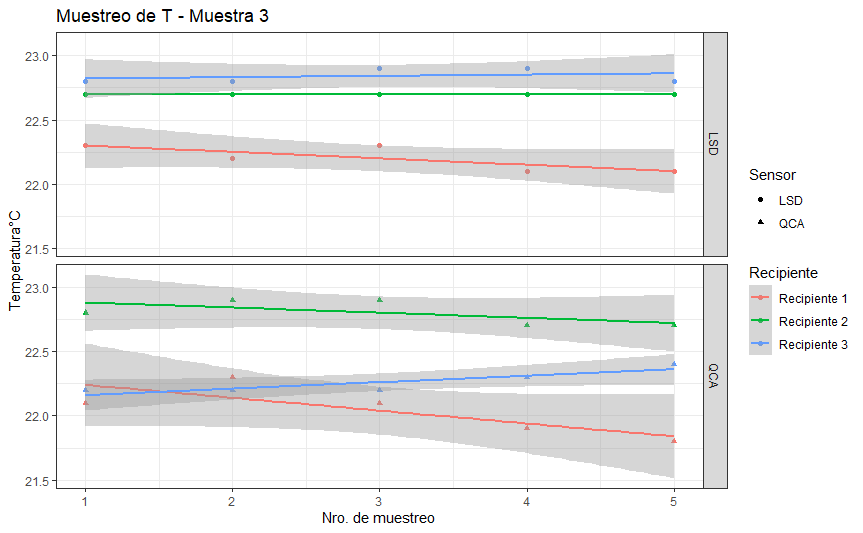
\includegraphics[width=0.75\linewidth]{Imagenes/cap4/T_M3.png}
        \caption {Muestreo de pH. }{\textbf{Fuente:}
        Elaboraci\'on Propia. }
        \label{fig:M3T}
    \end{figure}

\subsubsection{Muestra 3. Sensor Conductividad El\'ectrica}
  \begin{table}[H]
        \protect\caption[Muestra 3: Agua de laguna]{Muestra 3: Agua de laguna.}
        \label{tab:CEMuestra3}
        \centering
        \begin{tabular}{c c c}
            \hline
            \multicolumn{3}{c}{\textbf{Muestra 3: Agua de laguna.}} \\
             \hline
            \multicolumn{3}{c}{\textbf{Recipiente 1}} \\
            \hline
            \textbf{Lectura}&\textbf{LSD ($\mu S/cm$)}&\textbf{Qca ($\mu S/cm$)} \\
            \hline
            {1}& $36.35$&$50$ \\ 
            {2}& $35.18$&$52$ \\ 
            {3}& $35.15$&$50$ \\  
            {4}& $34.87$&$50$ \\ 
            {5}& $33.70$&$51$ \\
            \hline
            \multicolumn{3}{c}{\textbf{Recipiente 2}} \\
            \hline
            \textbf{Lectura}&\textbf{LSD ($\mu S/cm$)}&\textbf{Qca ($\mu S/cm$)} \\
            \hline
            {1}& $32.24$&$52$ \\ 
            {2}& $34.01$&$51$ \\ 
            {3}& $34.13$&$50$ \\  
            {4}& $33.03$&$53$ \\ 
            {5}& $32.75$&$52$ \\
            \hline
            \multicolumn{3}{c}{\textbf{Recipiente 3}} \\
            \hline
            \textbf{Lectura}&\textbf{LSD ($\mu S/cm$)}&\textbf{Qca ($\mu S/cm$)} \\
            \hline
            {1}& $37.39$&$51$ \\ 
            {2}& $36.75$&$50$ \\ 
            {3}&$39.31$&$50$\\  
            {4}& $44.40$&$53$\\ 
            {5}& $42.57$&$52$ \\
            \hline
        \end{tabular}
        \vspace{5mm}
        \newline
        \hfill \textbf{Fuente: }Elaboración Propia.
    \end{table}

% Gráfico CE3T
    \begin{figure}[H]
        \centering
        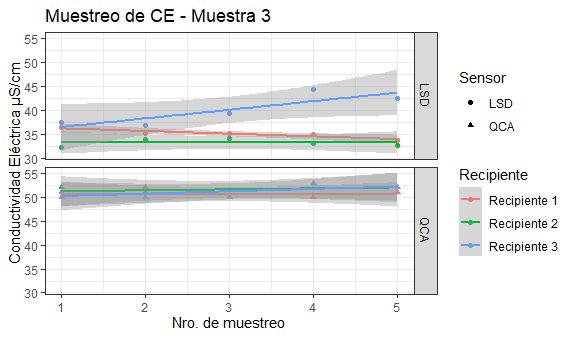
\includegraphics[width=0.75\linewidth]{Imagenes/cap4/CE_M3.png}
        \caption {Muestreo de conductividad el\'ectrica. }{\textbf{Fuente:}
        Elaboraci\'on Propia. }
        \label{fig:M3CE}
    \end{figure}

\subsubsection{Muestra 3. Sensor de pH}
%%%%% noooo
  \begin{table}[H]
        \protect\caption[Muestra 3: Agua de laguna]{Muestra 3: Agua de laguna.}
        \label{tab:TMuestra3}
        \centering
        \begin{tabular}{c c c}
            \hline
            \multicolumn{3}{c}{\textbf{Muestra 3: Agua de laguna.}} \\
             \hline
            \multicolumn{3}{c}{\textbf{Recipiente 1}} \\
            \hline
            \textbf{Lectura}&\textbf{LSD ($pH$)}&\textbf{Qca ($pH$)} \\
            \hline
            {1}& $6.302$&$6.99$ \\ 
            {2}& $6.285$&$6.98$ \\ 
            {3}& $6.318$&$6.96$ \\  
            {4}& $6.253$&$7.00$ \\ 
            {5}& $6.081$&$6.93$ \\
            \hline
            \multicolumn{3}{c}{\textbf{Recipiente 2}} \\
            \hline
            \textbf{Lectura}&\textbf{LSD ($pH$)}&\textbf{Qca ($pH$)} \\
            \hline
            {1}& $6.255$&$7.19$ \\ 
            {2}& $6.265$&$7.14$ \\ 
            {3}& $6.265$&$7.13$ \\  
            {4}& $6.138$&$7.10$ \\ 
            {5}& $6.138$&$7.20$ \\
            \multicolumn{3}{c}{\textbf{Recipiente 3}} \\
            \hline
            \textbf{Lectura}&\textbf{LSD ($pH$)}&\textbf{Qca ($pH$)} \\
            \hline
            {1}& $6.482$&$6.61$ \\ 
            {2}& $6.488$&$6.74$ \\ 
            {3}&$6.532$&$7.07$  \\  
            {4}& $6.538$&$7.01$ \\ 
            {5}& $6.522$&$7.20$ \\
            \hline
        \end{tabular}
        \vspace{5mm}
        \newline
        \hfill \textbf{Fuente: }Elaboración Propia.
    \end{table}

% Gráfico M3PH
\begin{figure}[H]
        \centering
        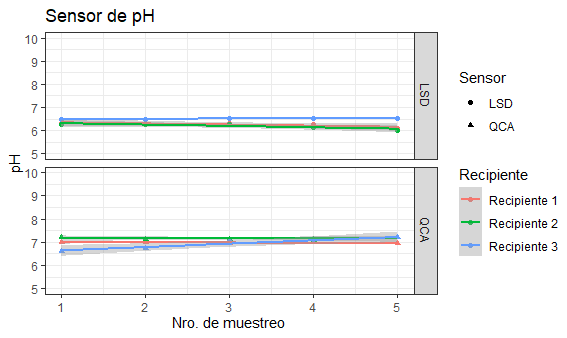
\includegraphics[width=0.75\linewidth]{Imagenes/cap4/pH_M3.png}
        \caption {Muestreo de pH. }{\textbf{Fuente:}
        Elaboraci\'on Propia. }
        \label{fig:M3PH}
\end{figure}

\subsection{An\'alsis de Datos. Muestra 3}

% Please add the following required packages to your document preamble:
% \usepackage{multirow}

\begin{table}[H]
\protect\caption[Muestra 3: Agua de laguna ]{Resumen de mediciones: Muestra 3.}
\label{tab:AnalisisM3}

\begin{tabular}{lccc|ccc}
\hline
Muestra 3 & 
\multicolumn{3}{c}{LSD}&
\multicolumn{3}{c}{QCA}\\ 
\textbf{\begin{tabular}[c]{@{}l@{}}An\'alisis de datos\end{tabular}} & \multicolumn{1}{c}{\begin{tabular}[c]{@{}c@{}}T \\ $^{\circ} C$\end{tabular}} & \multicolumn{1}{c}{pH}        & 
\begin{tabular}[c]{@{}c@{}}CE\\ $\mu S/cm$\end{tabular} & \multicolumn{1}{c}{\begin{tabular}[c]{@{}c@{}}T \\ $^{\circ} C$\end{tabular}} & \multicolumn{1}{c}{pH}        & 
\multicolumn{1}{c}{\begin{tabular}[c]{@{}c@{}}CE\\ $\mu S/cm$\end{tabular}}
\\ \hline
M\'inimo & \multicolumn{1}{c}{22.10}                            & \multicolumn{1}{c}{6.023} & 32.24                               & \multicolumn{1}{c}{21.80}                                       & 
\multicolumn{1}{c}{6.610} & 50.00   \\ M\'aximo                 & 
\multicolumn{1}{c}{22.90}                                       & 
\multicolumn{1}{c}{6.538} & 44.40                               & \multicolumn{1}{c}{22.90}                                       & 
\multicolumn{1}{c}{7.20}  & 53.00   \\ Promedio                 & 
\multicolumn{1}{c}{22.58}                                       & \multicolumn{1}{c}{6.316} & 36.12                               & \multicolumn{1}{c}{22.37}                                       & \multicolumn{1}{c}{7.017} & 51.13  \\ Desviación Est\'andar     & 
\multicolumn{1}{c}{0.291}                                       & \multicolumn{1}{c}{0.165} & 3.545                               & 
\multicolumn{1}{c}{0.354}                                       & 
\multicolumn{1}{c}{0.167}                                       & 
\multicolumn{1}{c}{1.125} \\ Varianza                           & \multicolumn{1}{c}{0.0845}                                      & \multicolumn{1}{c}{0.027} & 12.57                               & \multicolumn{1}{c}{0.125}                                       & 
\multicolumn{1}{c}{0.027}                                       & 
\multicolumn{1}{c}{1.267}  \\ Error Estándar                    & \multicolumn{1}{c}{0.075}                                       & \multicolumn{1}{c}{0.0426} & 0.915                              & 
\multicolumn{1}{c}{0.0914}                                      & 
\multicolumn{1}{c}{0.0431}                                      & 
\multicolumn{1}{c|}{0.290}  \\ 
\hline
\end{tabular}
\end{table}

En la tabla \ref{tab:AnalisisM3}, se puede observar algunos par\'ametros estad\'isticos calculados, a partir de los registros recolectados en el muestreo de los recipientes de la muestra 3, el cual arrojo los siguientes resultados. 
La desviaci\'on est\'andar m\'as elevada se registr\'o en el par\'ametro de conductividad el\'ectrica, siendo el mayor el registrado por el sensor de LSD, igual a 3.545 un  3.17\%  mayor a la desviación del sensor de QCA, en los resultados de  los otros par\'ametros, se registra un desviaci\'on parecidas siendo los menor en sensores de LSD,   . 
La varianza sigue la misma tendencia de la desviaci\'on est\'andar, la conductividad el\'ectrica presenta una mayor dispersi\'on. 
El error est\'andar, presenta valores bajos en todos los par\'ametros menores a 1, el cual sugiere que los valores recolectados son uniforme y se encuentran cerca de la media. 
Los valores mínimos recolectados en el caso de la temperatura presentan una deferencia de 0,3 $ ^{\circ}C$ siendo 21.3$ ^{\circ}C$ la menor lectura registrada por el sensor de QCA, en el caso del pH la diferencia entre los mínimos fue de 0,587 pH, siendo 6,023 pH la menor lectura registrada por el sensor de LSD, la m\'inima conductividad el\'ectrica registrado fue de 32,24 $\mu S/cm$ con una diferencia de 17,76 $\mu S/cm$ con respecto al sensor de QCA. 
Los valores m\'aximo recolectados en el caso de la temperatura no presentaron  deferencia siendo 22,90 $ ^{\circ}C$ la  lectura registrada por los sensores, en el caso del pH la diferencia entre los m\'aximos fue de 0.662 pH, siendo 7.2 pH la mayor lectura registrada por el sensor de QCA, la conductividad el\'ectrica m\'as alta registrada fue de 53 $\mu S/cm$ con con una diferencia de 8.6 $\mu S/cm$ con respecto a la mayor lectura registrada en el sensor QCA.
El promedio de las mediciones fueron cercanas con una diferencia de 9 $\%$ en el caso del pH, siendo el promedio de los datos de pH registrado por el sensor de QCA 7,017 pH contra el promedio de pH registrado por el sensor LSD igual a 6.316 pH, en el caso de los resultados promedios registrados de la temperatura la diferencia entre los resultados fue menor al 0.93$\%$ siendo la temperatura promedio del sensor LSD igual a 22.58$ ^{\circ}C$ y la temperatura promedio del sensor de QCA igual a 22.37$^{\circ}C$, los promedio de las mediciones de los sensores de conductividad eléctrica entre los sensores tienen diferencia de 29.35 $\%$, siendo el promedio de los datos de CE registrado por el sensor de QCA 51.13 contra el promedio de CE registrado por el sensor LSD igual a 36.12 $\mu S/cm$.
En este an\'alisis de datos correspondiente a la muestra 3, se observan los mismos patrones, los resultados finales con valores cercanos, con un margen de diferencia menor al 7\% entre ambos sensores de ph - T y menor al 23.35 \% en el sensor de CE.

\begin{table}[H]
\caption{Relaci\'on entre los equipos de sensores}
\label{tab:VaCoM3}
\centering
\begin{tabular}{llll} 
\toprule
& T   &  pH    & CE \\
\midrule
Covarianza  & 0.05483 & 0.0073 & 0.157                \\
Correlación & 0.5483& 0.3782 & 0.628        \\
\bottomrule
\end{tabular}
\\ \textbf{Fuente: }Elaboración Propia.
\end{table}  

En un an\'alisis de la tabla \ref{tab:VaCoM2}, donde se encuentran los resultados de covarianza y correlación de las muestras, en el caso de la temperatura, conductividad el\'ectrica y pH se obtuvieron unos valores de covarianzas positivas el cual indica que ambas lecturas varían en la misma dirección, as\'i mismo en los tres par\'ametros se obtuvieron correlaciones positivas menores a 1, refleja que se da una correlación positiva entre sí, la media varía en la misma dirección con el factor del valor del coeficiente de correlación. Luego de analizar los resultados obtenidos en el caso de la muestra 3, se puede concluir que ambos sensores presentan lecturas cercanas,relacionadas entre s\'i, con baja dispersi\'on. 

% resumen de mediciones

%Estadistica de mediciones

\section{Pruebas de campo}
Las pruebas en campo se realizaron con el fin de verificar el comportamiento de la sonda y sistemas en un entorno de trabajo real. 
Se realizaron varias pruebas de campos en el lago Ypakarai, los cuales ayudaron a mejorar el dise\~no final, desde el punto de hardware y software, alguna de las mejoras fueron,laincorporaci\'on de una estructura interna de fijado por la base de la sonda, a modo de sostener y mantener ordenado todos los elementos electr\'onicos, evitando con esto que se puedan da\~nar por su manipulaci\'on, incorporaci\'on de un o-ring para mejorar el hermetismo e impedir el ingreso de l\'iquidos, ya que luego de las primeras pruebas se detectaron filtraciones provenientes de la rosca principal uni\'on base-anillo,para la publicaci\'on remota, se agreg\'o al c\'odigo principal, rutinas multi hilos, para cuando la sonda pierda conexi\'on a internet no se pierdan estos paquetes durante, y unan vez recuperada la conexi\'on se env\'ien todos los hilos.

\begin{figure}[H]
     \centering
     \begin{subfigure}[b]{0.65\textwidth}
         \centering
         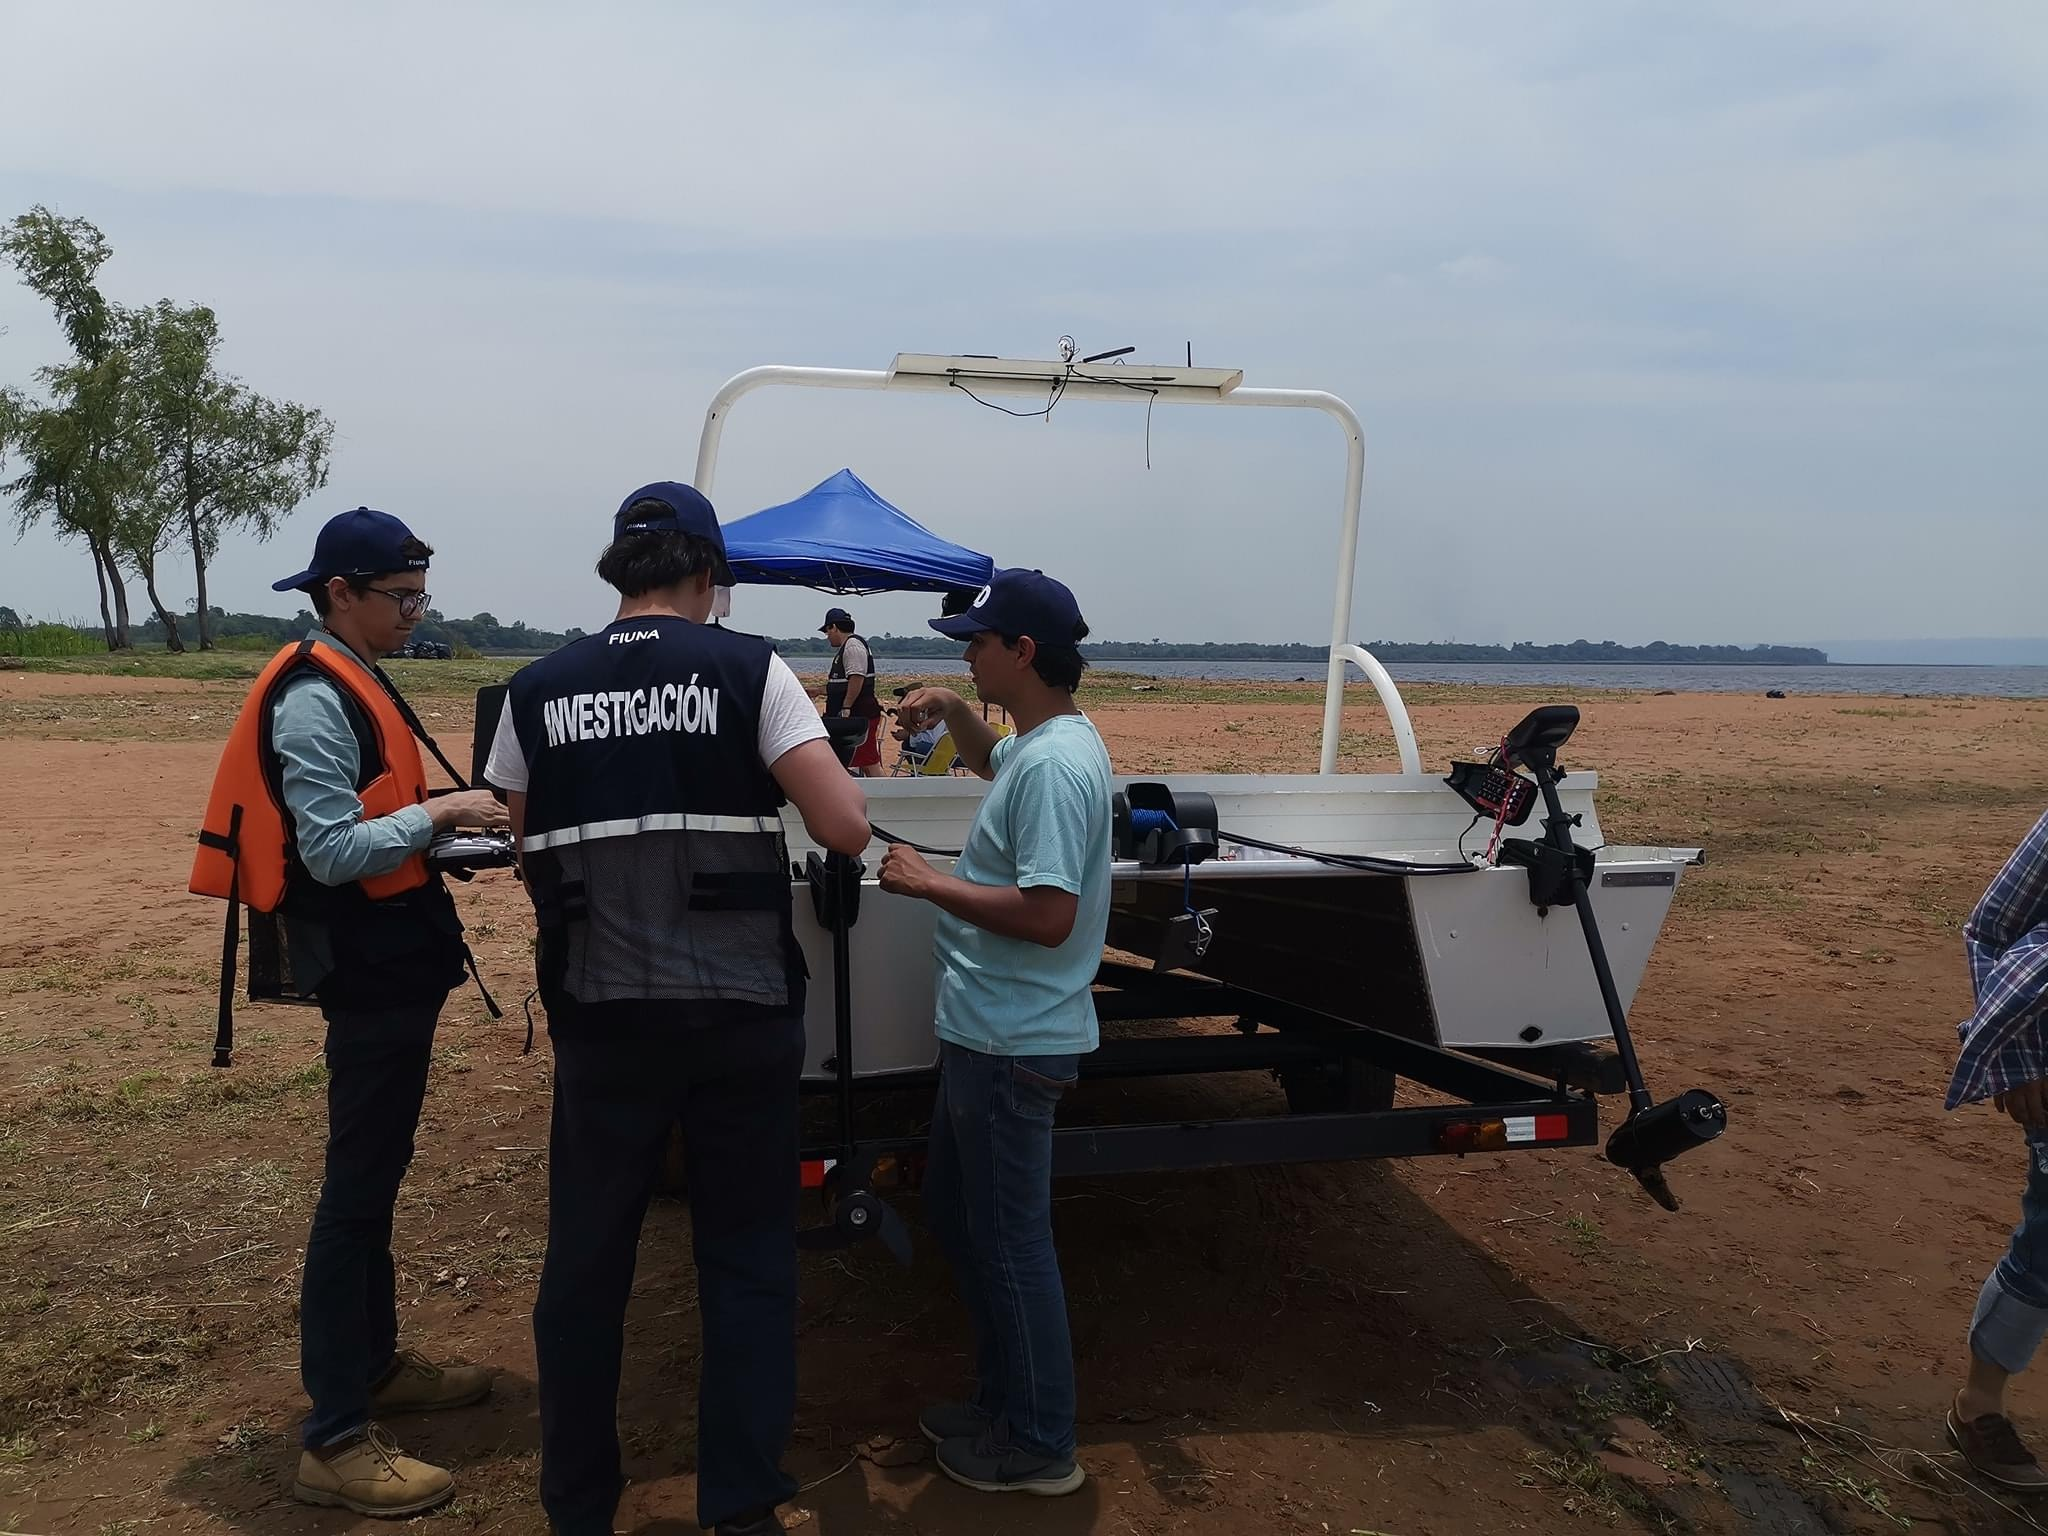
\includegraphics[width=\textwidth]{Imagenes/cap4/PruebaCampo.jpeg}
         \caption{Preparaci\'on del ASV.}
         \label{fig:PreparacionASV}
     \end{subfigure}
     \hfill
     \begin{subfigure}[b]{0.3\textwidth}
         \centering
         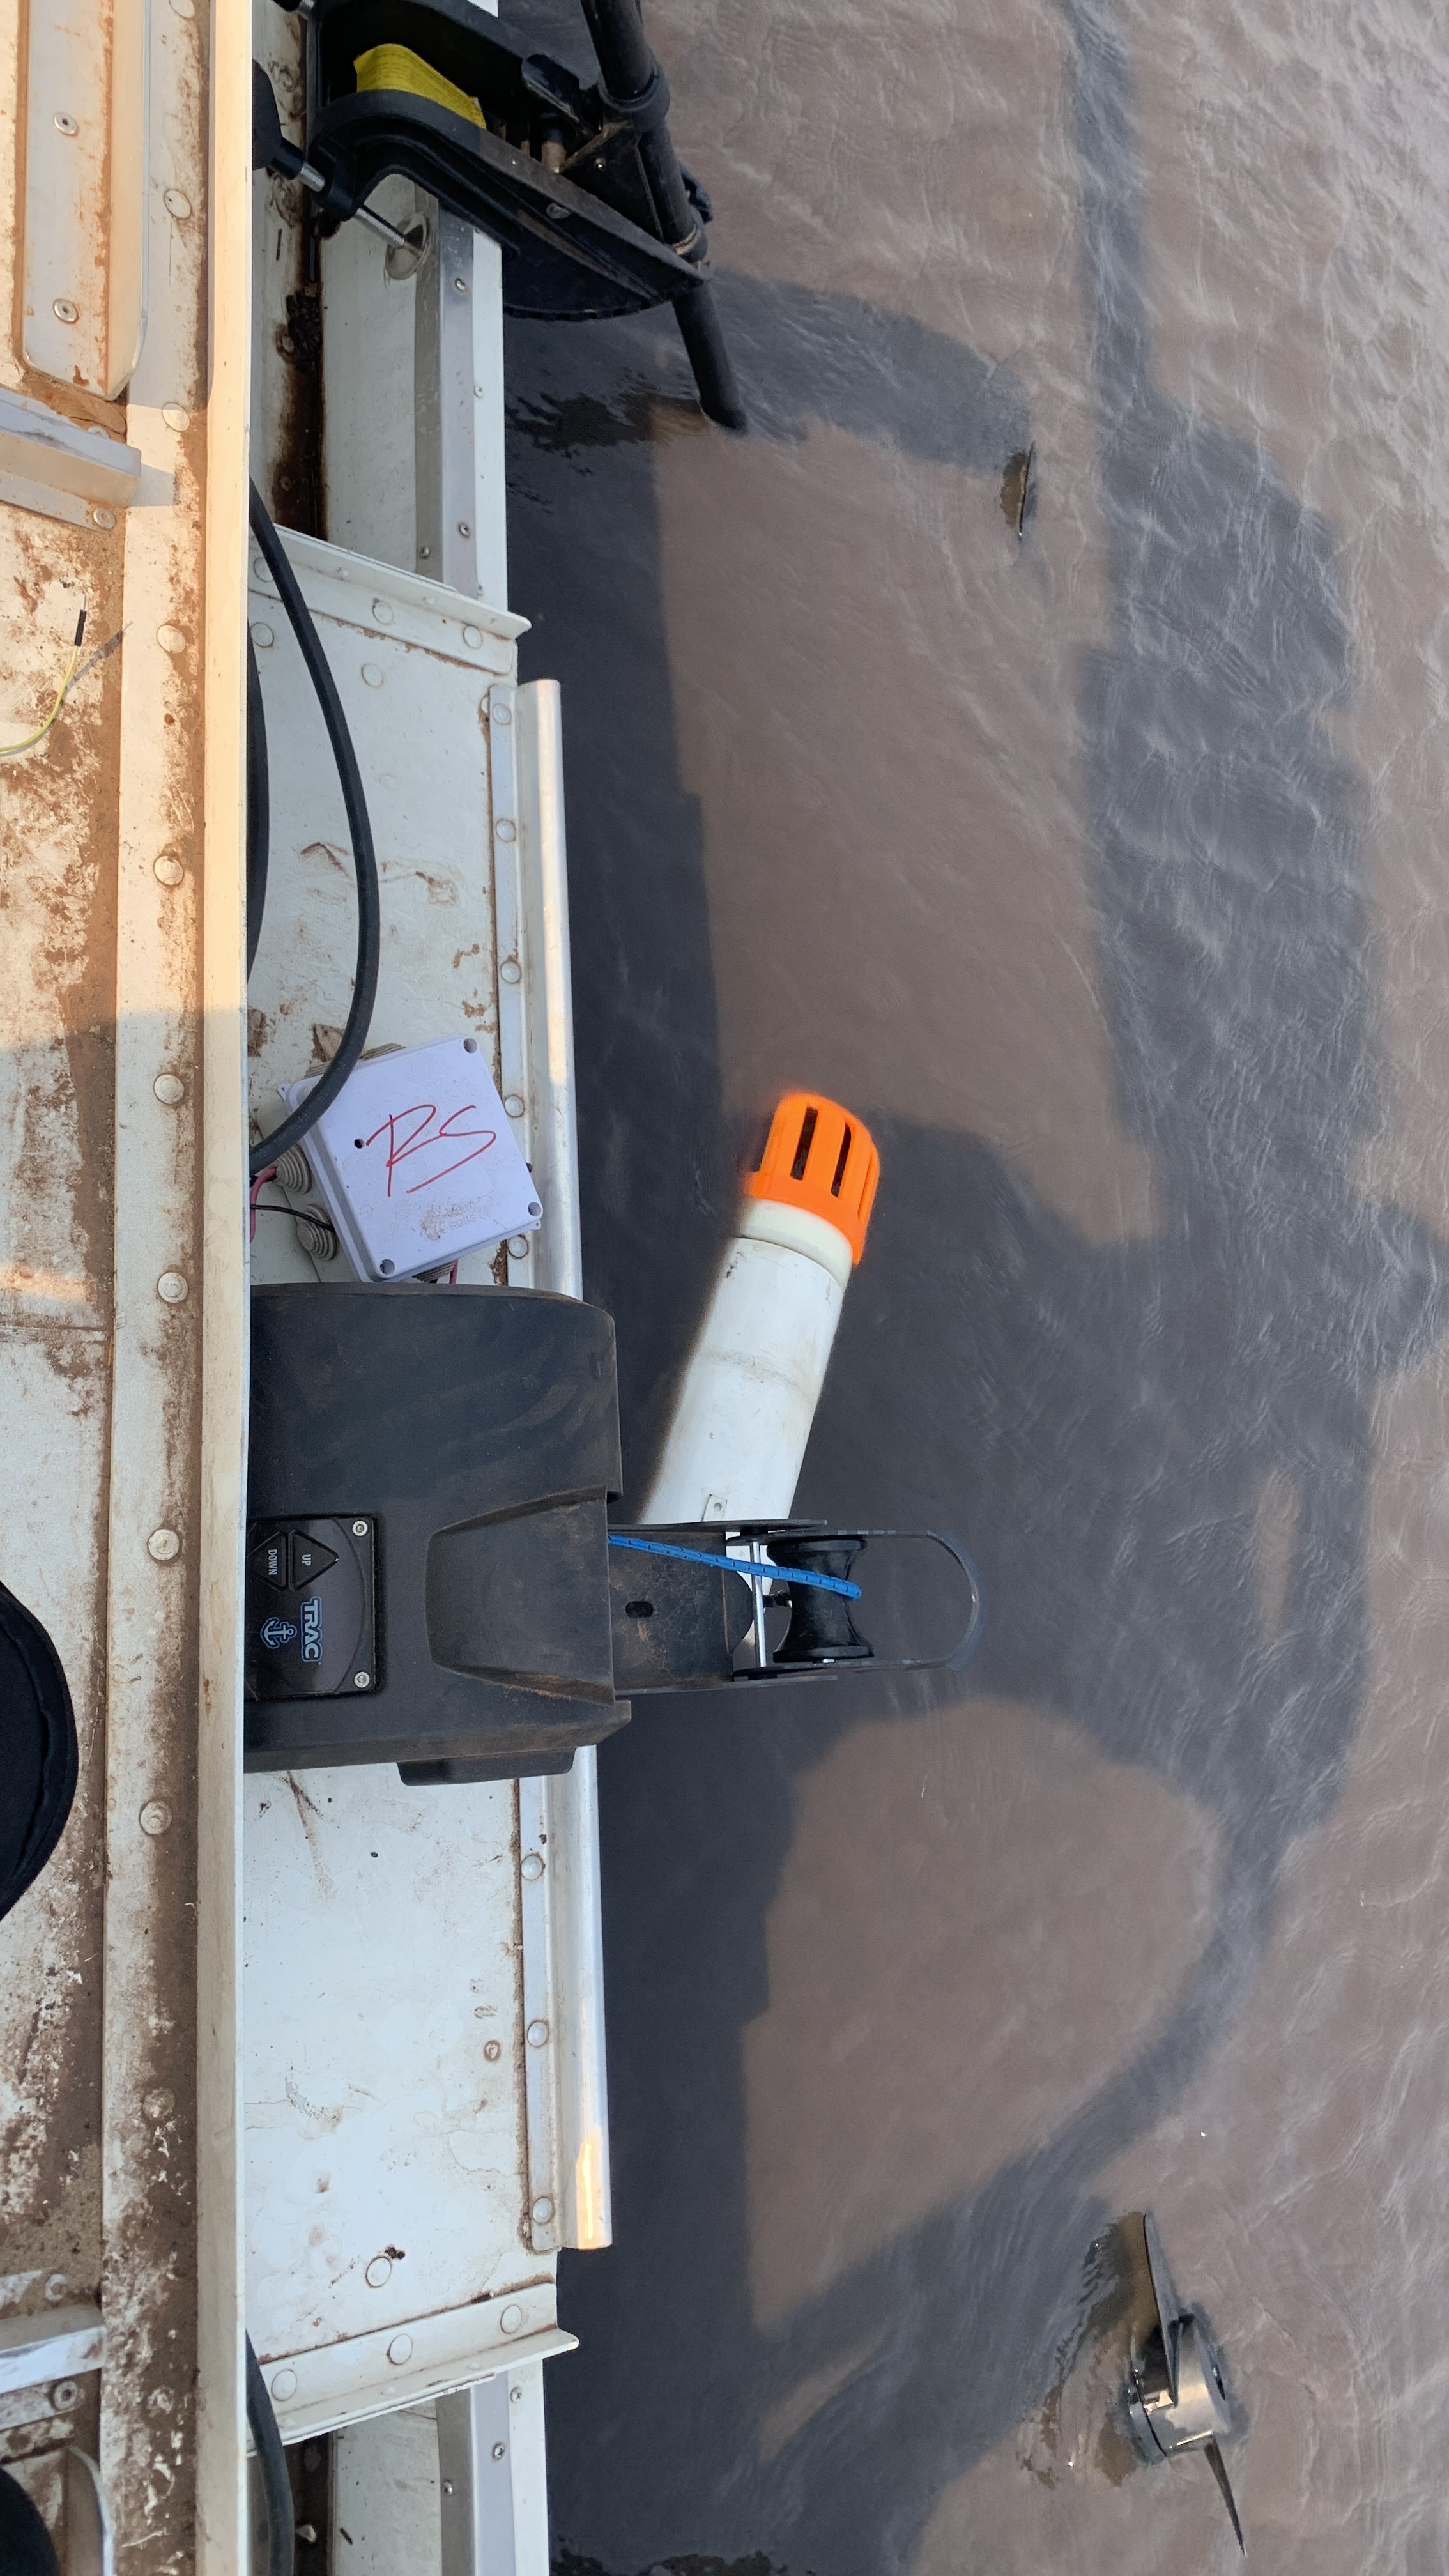
\includegraphics[width=\textwidth]{Imagenes/cap4/PruebaCampo1.JPG}
         \caption{Sonda instalada en el ASV.}
         \label{fig:SondaASV}
     \end{subfigure}
     \hfill
    \caption{Prueba de campo - Lago Ypakarai}
    \label{fig:PruebaCampo}
\end{figure}


\subsection{Muestreo de pH. Prueba de Campo}

\begin{figure}[H]
        \centering
        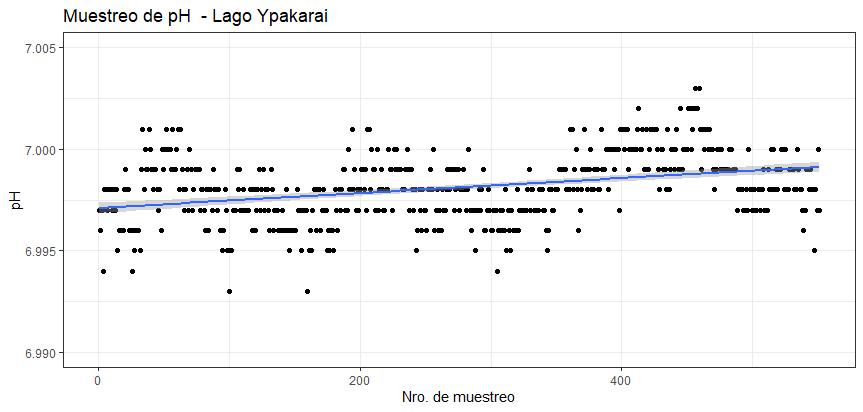
\includegraphics[width=0.75\linewidth]{Imagenes/cap4/pHLago.png}
        \caption {Muestreo de pH, lago Ypakarai. }{\textbf{Fuente:}
        Elaboraci\'on Propia. }
        \label{fig:Lago_ph}
\end{figure}

La Resoluci\'on. SEAM N$ ^{\circ}$ 222/02 estable un l\'imite inferior y superior igual a 6 y 9 respectivamente.Durante esta campa\~na todos los puntos se encuentran acorde a la normativa.
En la tabla \ref{table:Lago_ph} se presenta un an\'alisis comparativo de los valores obtenidos para el par\'ametro pH correspondientes a la prueba de campo  realizada.

\begin{table}[H]
\centering
\caption{Prueba de campo. Estadísticas descriptivas – ph}
\label{table:Lago_ph}
\begin{tabular}{lrrrr}
\toprule & 
\multicolumn{3}{r}{Rango} \\ \cline{4-5} & 
Muestras & Promedio & Mínimo & Máximo \\
\midrule
Prueba de campo  &      472 &      7.0 &  6.993 &  7.003 \\
\bottomrule
\end{tabular}
\end{table}
Se realizaron 472 mediciones en todo el recorrido, los valores recolectados de potencial de hidr\'ogeno que oscilan en un intervalo entre 6.993 y 7.003.
En la tercera \cite{3er_Cemit} y cuarta \cite{4to_Cemit} campaña de muestreo del “Monitoreo de Calidad de Agua por Campañas de Muestreo en el Lago Ypacaraí 2019 -2021, correspondientes al periodo de la prueba de campo, realizado por CEMIT-UNA, segun contrato ITAIPÚ/UNA No. 4500054462/2019, se documentan promedios de pH que oscilaron entre 6.0 y 7.98. 
Se verifica que par\'ametro recolectados en esta campa\~na se encuentra dentro del intervalo de valores.

\subsection{Muestreo de CE. Prueba de Campo}

\begin{figure}[H]
        \centering
        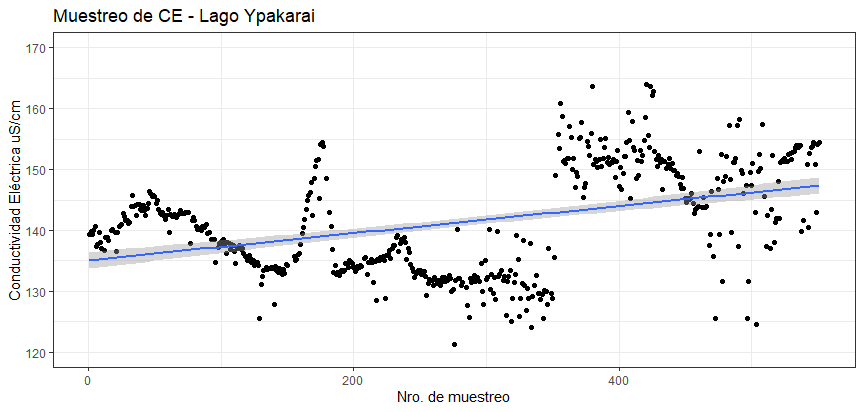
\includegraphics[width=0.75\linewidth]{Imagenes/cap4/CE_lago.png}
        \caption {Muestreo de CE, lago Ypakarai. }{\textbf{Fuente:}
        Elaboraci\'on Propia. }
        \label{fig:Lago_ce}
\end{figure}

Para aguas de Clase 2 la Resoluci\'on 222/02 no estable ningún l\'imite para el par\'ametro evaluado; se toma como referencia el l\'mite de 1250 $\mu S/cm$ establecido en el Anexo X de la ley 1614/2000 en cual Ley General Del Marco Regulatorio y Tarifario Del Servicio De Agua Potabley Alcantarillado Sanitario. Todas las determinaciones realizadas en la campa\~na se encuentran en conformidad con la normativa de referencia.
En la tabla \ref{table:Lago_ce} se presenta un an\'alisis comparativo de los valores obtenidos para el par\'ametro CE correspondientes a la prueba de campo  realizada.

\begin{table}[H]
\centering
\caption{Prueba de campo. Estadísticas descriptivas – ce}
\label{table:Lago_ce}
\begin{tabular}{lrrrr}
\toprule& 
\multicolumn{3}{r}{Rango} \\  \cline{4-5}& 
Muestras & Promedio & Mínimo & Máximo \\
\midrule
Prueba de campo  &      472 &   137.65 &   4.62 &  163.6 \\
\bottomrule
\end{tabular}
\end{table}

Se realizaron 472 mediciones en todo el recorrido, los valores recolectados de conductividad el\'ectrica que oscilan en  un intervalo entre 4.62 $\mu S/cm$ y 163.6 $\mu S/cm$, en promedio 137.65 $\mu S/cm$.
En la tercera \cite{3er_Cemit} y cuarta \cite{4to_Cemit} campaña de muestreo del “Monitoreo de Calidad de Agua por Campañas de Muestreo en el Lago Ypacaraí 2019 -2021, correspondientes al periodo de la prueba de campo, realizado por CEMIT-UNA, segun contrato ITAIPÚ/UNA No. 4500054462/2019, se documentan promedios de CE que oscilaron entre $156 \mu S/cm$ y $601 \mu S/cm$. 
Se verifica que los datos del par\'ametro, recolectados en esta campa\~na se encuentra dentro del intervalo de valores.

\subsection{Muestreo de OD. Prueba de Campo}

\begin{figure}[H]
        \centering
        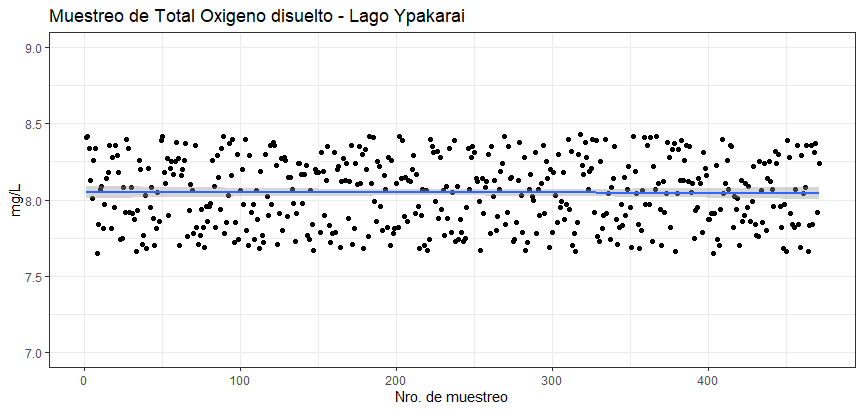
\includegraphics[width=0.75\linewidth]{Imagenes/cap4/OD_Lago Ypakarai.png}
        \caption {Muestreo de OD, lago Ypakarai.}{\textbf{Fuente:}
        Elaboraci\'on Propia. }
        \label{fig:Lago_od}
\end{figure}

La Resoluci\'on SEAM 222/02 establece que el ox\'igeno disuelto en aguas de clases 2 debe ser  $> 5 mg O_2/L$. Todas las determinaciones realizadas en la campa\~na se encuentran en conformidad con la normativa de referencia.
En la tabla \ref{table:Lago_od} se presenta un an\'alisis comparativo de los valores obtenidos para el par\'ametro OD correspondientes a la prueba de campo  realizada.

\begin{table}[H]
\centering
\caption{Prueba de campo. Estadísticas descriptivas – OD}
\label{table:Lago_od}
\begin{tabular}{lrrrr}
\toprule
          & \multicolumn{3}{r}{Rango} \\ \cline{4-5}
          & Muestras & Promedio & Mínimo & Máximo \\
\midrule
Prueba de campo  &      472 &     8.05 &   7.65 &   8.43 \\
\bottomrule
\end{tabular}
\end{table}

Se realizaron 472 mediciones en todo el recorrido, los valores recolectados de oxigeno disuelto que oscilan en  un intervalo entre 7.65   y 8.43 $mg/L$, en promedio 8.05 $mg/L$.
En la tercera \cite{3er_Cemit} y cuarta \cite{4to_Cemit} campaña de muestreo del “Monitoreo de Calidad de Agua por Campañas de Muestreo en el Lago Ypacaraí 2019 -2021, correspondientes al periodo de la prueba de campo, realizado por CEMIT-UNA, segun contrato ITAIPÚ/UNA No. 4500054462/2019, se documentan promedios de CE que oscilaron entre 7.85 $mg/L$ y 8.9 $mg/L$. 
Se verifica que los datos del par\'ametro, recolectados en esta campa\~na se encuentra dentro del intervalo de valores.

\subsection{Muestreo de OPR. Prueba de Campo}

\begin{figure}[H]
        \centering
        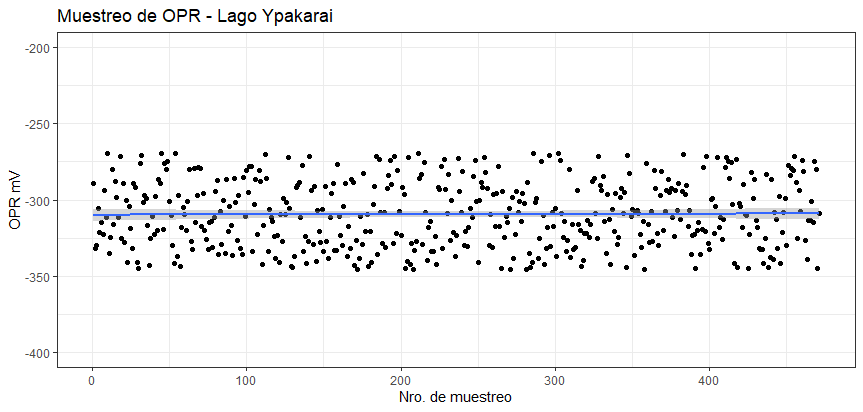
\includegraphics[width=0.75\linewidth]{Imagenes/cap4/OPR_LAGO.png}
        \caption {Muestreo de OPR, lago Ypakarai. }{\textbf{Fuente:}
        Elaboraci\'on Propia. }
        \label{fig:Lago_opr}
\end{figure}
La Resoluci\'on. SEAM N$ ^{\circ}$ 222/02 no define un valor límite para OPR La Organización Mundial de la Salud adoptó en 1972 la medida del POTENCIAL REDOX como la medida más fiable para medir la calidad sanitaria del agua potable, estableciendo en \cite{OPR_10665-39989} el valor 650mV como valor adecuado para el agua potable.
En la tabla \ref{table:Lago_temp} se presenta un an\'alisis comparativo de los valores obtenidos para el par\'ametro OPR correspondientes a la prueba de campo realizada. 
\begin{table}[H]
\centering
\caption{Prueba de campo. Estadísticas descriptivas – OPR}
\label{table:Lago_opr}
\begin{tabular}{lrrrr}
\toprule
          & \multicolumn{3}{r}{Rango} \\  \cline{4-5}
          & Muestras & Promedio & Mínimo & Máximo \\
\midrule
Prueba de campo  &      472 &  -309.43 & -345.7 & -269.1 \\
\bottomrule
\end{tabular}
\end{table}

Se realizaron 472 mediciones en todo el recorrido, los valores recolectados de oxigeno disuelto que oscilan en  un intervalo entre -259.1 $mV$ y -345.7 $mV$, en promedio -309.4 $mV$.

\subsection{Muestreo de T. Prueba de Campo}

\begin{figure}[H]
        \centering
        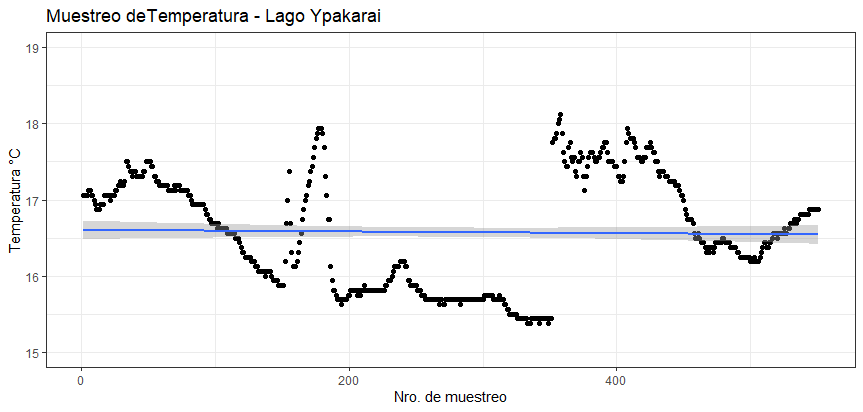
\includegraphics[width=0.75\linewidth]{Imagenes/cap4/Temp_lago.png}
        \caption {Muestreo de T, lago Ypakarai. }{\textbf{Fuente:}
        Elaboraci\'on Propia. }
        \label{fig:Lago_temp}
\end{figure}

La Resoluci\'on. SEAM N$ ^{\circ}$ 222/02 no define un valor límite para la temperatura de las aguas de Clase 2; solo para el vertido de efluentes a cuerpos receptores se establece un valor límite de 40$ ^{\circ}$C.
En la tabla \ref{table:Lago_temp} se presenta un an\'alisis comparativo de los valores obtenidos para el par\'ametro T correspondientes a la prueba de campo  realizada.

\begin{table}[H]
\centering
\caption{Prueba de campo. Estadísticas descriptivas – temp}
\label{table:Lago_temp}
\begin{tabular}{lrrrr}
\toprule
          & \multicolumn{3}{r}{Rango} \\ \cline{4-5}
          & Muestras & Promedio & Mínimo & Máximo \\
\midrule
Prueba de campo  &      472 &    16.51 & 15.375 & 18.125 \\
\bottomrule
\end{tabular}
\end{table}

Se realizaron 472 mediciones en todo el recorrido, los valores recolectados de temperatura que oscilan en  un intervalo entre 15.37 $ ^{\circ}$C y 18.12 $ ^{\circ}$C, en promedio 16.51 $^{\circ}$C .
En la tercera \cite{3er_Cemit} y cuarta \cite{4to_Cemit} campaña de muestreo del “Monitoreo de Calidad de Agua por Campañas de Muestreo en el Lago Ypacaraí 2019 -2021, correspondientes al periodo de la prueba de campo, realizado por CEMIT-UNA, segun contrato ITAIPÚ/UNA No. 4500054462/2019, se documentan promedios de T que oscilaron entre 19.7 $ ^{\circ}$C y 26.2 $ ^{\circ}$C. 
Se verifica que los datos del par\'ametro, recolectados en esta campa\~na no se encuentra dentro del intervalo de valores.

\subsection{Muestreo de TDS. Prueba de Campo}

\begin{figure}[H]
        \centering
        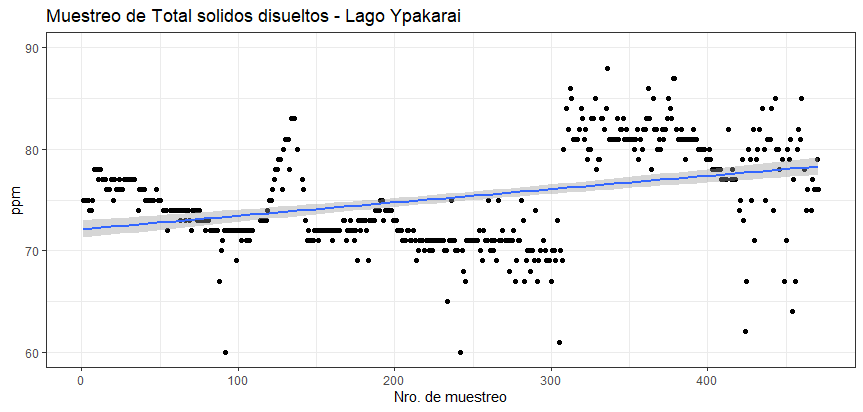
\includegraphics[width=0.75\linewidth]{Imagenes/cap4/TDS LagoYpakarai.png}
        \caption {Muestreo de TDS, lago Ypakarai. }{\textbf{Fuente:}
        Elaboraci\'on Propia. }
        \label{fig:Lago_tds}
\end{figure}

La Resoluci\'on SEAM 222/02 establece que el total de solidos disuelto en aguas de aguas del territorio nacional ser menor a  500$ mg /L$. Todas las determinaciones realizadas en la campa\~na se encuentran en conformidad con la normativa de referencia.
En la tabla \ref{table:Lago_tds} se presenta un an\'alisis comparativo de los valores obtenidos para el par\'ametro TDS correspondientes a la prueba de campo  realizada.

\begin{table}[H]
\centering
\caption{Prueba de campo. Estadísticas descriptivas – tds}
\label{table:Lago_tds}
\begin{tabular}{lrrrr}
\toprule
          & \multicolumn{3}{r}{Rango} \\ \cline{4-5}
          & Muestras & Promedio & Mínimo & Máximo \\
\midrule
Prueba de campo  &      472 &    73.86 &    2.0 &   88.0 \\
\bottomrule
\end{tabular}
\end{table}

\subsubsection{Resumen del an\'alsis de Datos. Prueba de Campo}
A continuaci\'on se presenta un resumen de todos los datos obtenidos.
El muestreo se hizo durante el desplazamiento en un circuito cerrado partiendo de la playa municipal de San Bernardino, pasando por el centro del lago Ypakarai  y la desembocadura del arrollo Piray\'u, tal como se puede observar en la figura \ref{fig:ruta}, el muestreo inicio a las 10:00hs hasta las 12:25hs, durante este periodo se registraron 471 (cuatrocientos setenta y uno) muestras, en intervalos aproximados de 25 segundos, los par\'ametros  recolectados durante el muestreo de pH, conductividad el\'ectrica, ox\'igeno disuelto, total de s\'olidos disueltos, potencial \'oxido reducci\'on y temperatura, los datos de georeferenciaci\'on fueron prove\'idos por el ASV en cada punto de muestreo.
\begin{figure}[H]
        \centering
        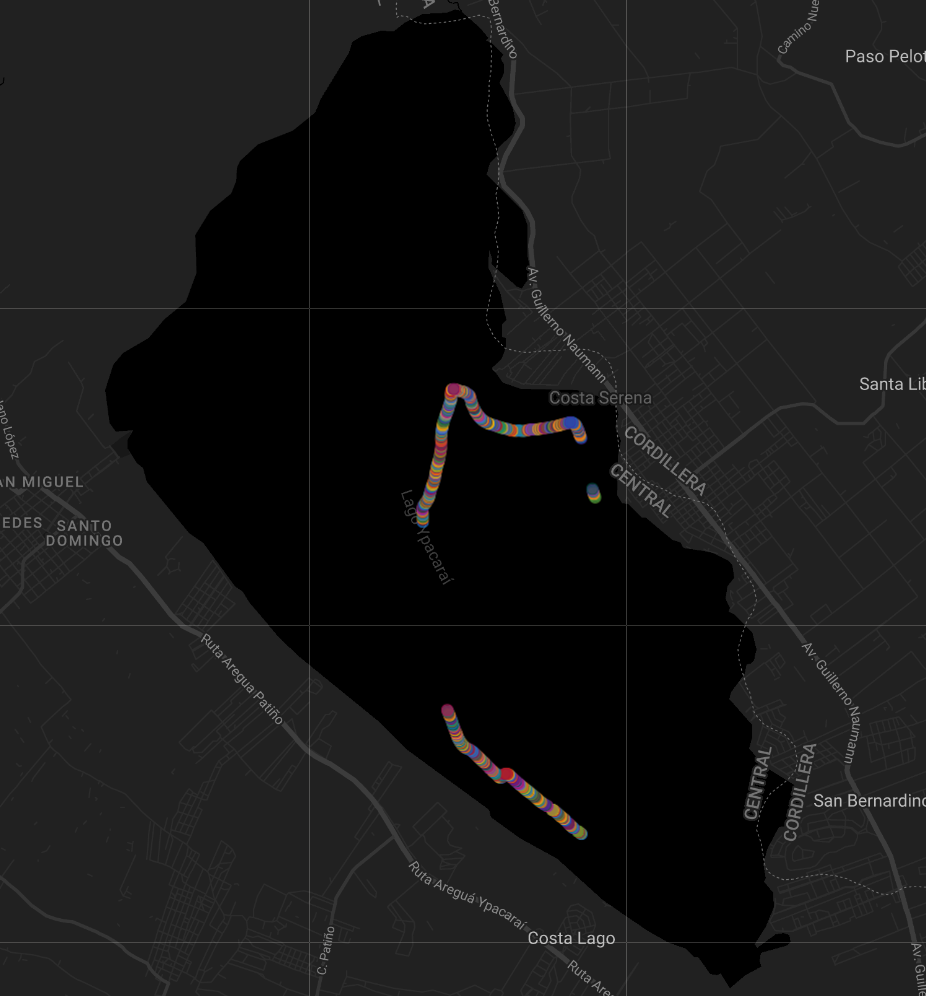
\includegraphics[scale=0.7]{Imagenes/cap4/Recorrido.png}
        \caption {Ruta de muestreo. }{\textbf{Fuente:}
        Elaboraci\'on Propia. }
        \label{fig:ruta}
\end{figure}

En la tabla \ref{tab:datos Lago}, se presenta los rsultados de unos an\'alisis estadísticos descriptivos correspondientes a todos los par\'ametros de la prueba de campo realizada.

\begin{table}[H]
\caption{Muestreo lago Ypakarai. Resumen}
\label{tab:datos Lago}
\begin{tabular}{lllllll} \hline& 
T  $^{\circ}C$ & $pH$     & CE $\mu S/cm$ & TDS $ppm$ & OPR $mV$ & OD $mgL/$  \\ \hline
M\'inimo & 15.37 & 6.993 & 4.62 & 2    & -345.70  & 7.65     \\
M\'aximo & 18.12 & 7.0   & 163.6    & 88    & -269.10  & 8.43 \\
Promedio & 16.51  & 6.99 & 137.65 & 73.85 & -309.42  & 8.047 \\
Desv. est. & 0.748 & 0.0016   & 17.50   & 9.46     & 21.634   & 0.22     \\
Varianza                & 0.56           & 0.000003 & 777.14        & 225.07    & 468.03   & 0.050296 \\
Error est.               & 0.034 & 0.000076 & 1.283154 & 0.690544 & 0.995786 & 0.010323 \\
\hline
\end{tabular}
\end{table}
Los temperatura maxima registrada fye de 18.12 $^o$C, el potencial de hidrigeno maximo fue de 7pH, el valor maximo de la conductividad electrica fue de 163.6 $\mu S/cm$, el valor maximo de TDS fue 88ppm, en el caso de OPR fue -269.10 $mV$ y el oxigeno disuelto macimo resgrado fue 0.22 $mg/L$.
Se puede apreciar que los sensores de temperatura, pH, y oxigeno disuelto presentaron resultados de desviación estándar mas bajos, por lo tanto menos disperso. En el caso de la conductividad eléctrica, total de solidos disueltos y opr, presentaron valores de desviación estándar mas altas, por lo que se concluye de su comportamiento mas disperso.
El error estándar calculado es bajo para todas las medicines. 
Todo los datos obtenidos se encuentran en el intervalo de valores obtenidos en otras campa\~nas de muestreo como ser lo desarrollados por CEMIT- Itaipu \cite{3er_Cemit}\cite{4to_Cemit}, realizados en un periodo cercano a esta prueba de campo, y también se encuentran dentro de los valores obtenidos en \cite{lopez_moreira_m_eutrophication_2018}, donde se analizaron algunos de estos parámetros.  

\section{Interfaz de monitoreo}
La interfaz gr\'afica fue desarrollada con el objetivo de ofrecer una pre visualizaci\'on de los datos recolectados en tiempo de ejecucion, sin tener que acceder directamente a la base de datos, que sea de f\'acil uso y compatible con la mayor cantidad de dispositivos posibles.
Con la tecnolog\'ia NodeRed, fue posible instalar la interfaz gr\'fica mediantes nodos y con el protocolo de comunicaci\'on  MQTT lograr capturar los datos enviados por los t\'opicos antes  establecidos, \appendixautorefname{appendix: Topicos}
La interfaz gr\'afica es multi plataforma, compatibles con todos los sistemas operativos m\'oviles como de escritorio, ya que al ser una aplicaci\'on web instalada en servidores, es compatible con cualquier dispositivo que tenga instalado alg\'un navegador web donde se ejecutarse. En la figura \ref{fig:Monitoreo} se puede apreciar la interfaz gráfica fue instalada en el raspberry de la sonda y en la sala de monitoreo del laboratorio de sistemas distribuidos de fiuna ubicado en CITEC. 
\begin{figure}[H]
        \centering
        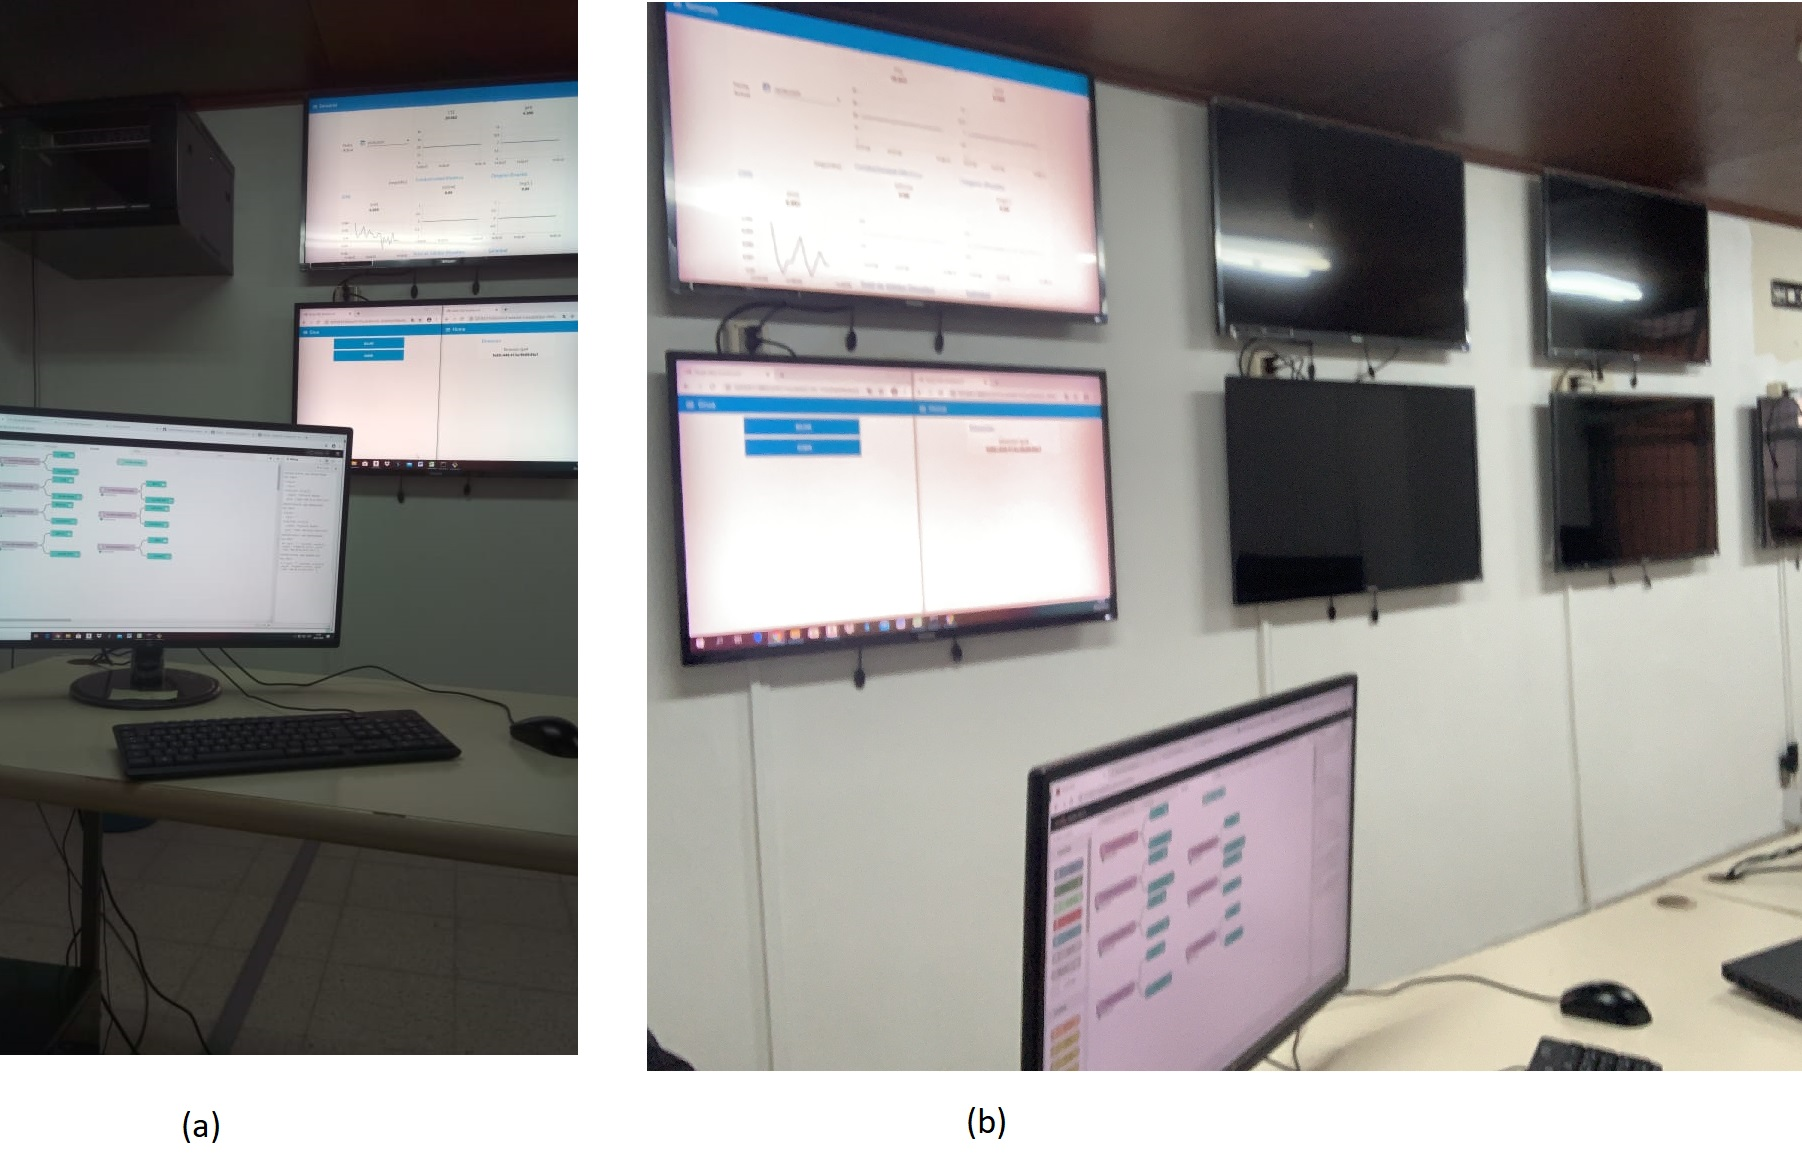
\includegraphics[scale=0.7]{Imagenes/cap4/SalaMonitoreo.jpg}
        \caption {Implementaci\'on de interfaz en la sala de monitoreo CITEC. }{\textbf{Fuente:}
        Elaboraci\'on Propia. }
        \label{fig:Monitoreo}
\end{figure}


\begin{figure}[H]
        \centering
        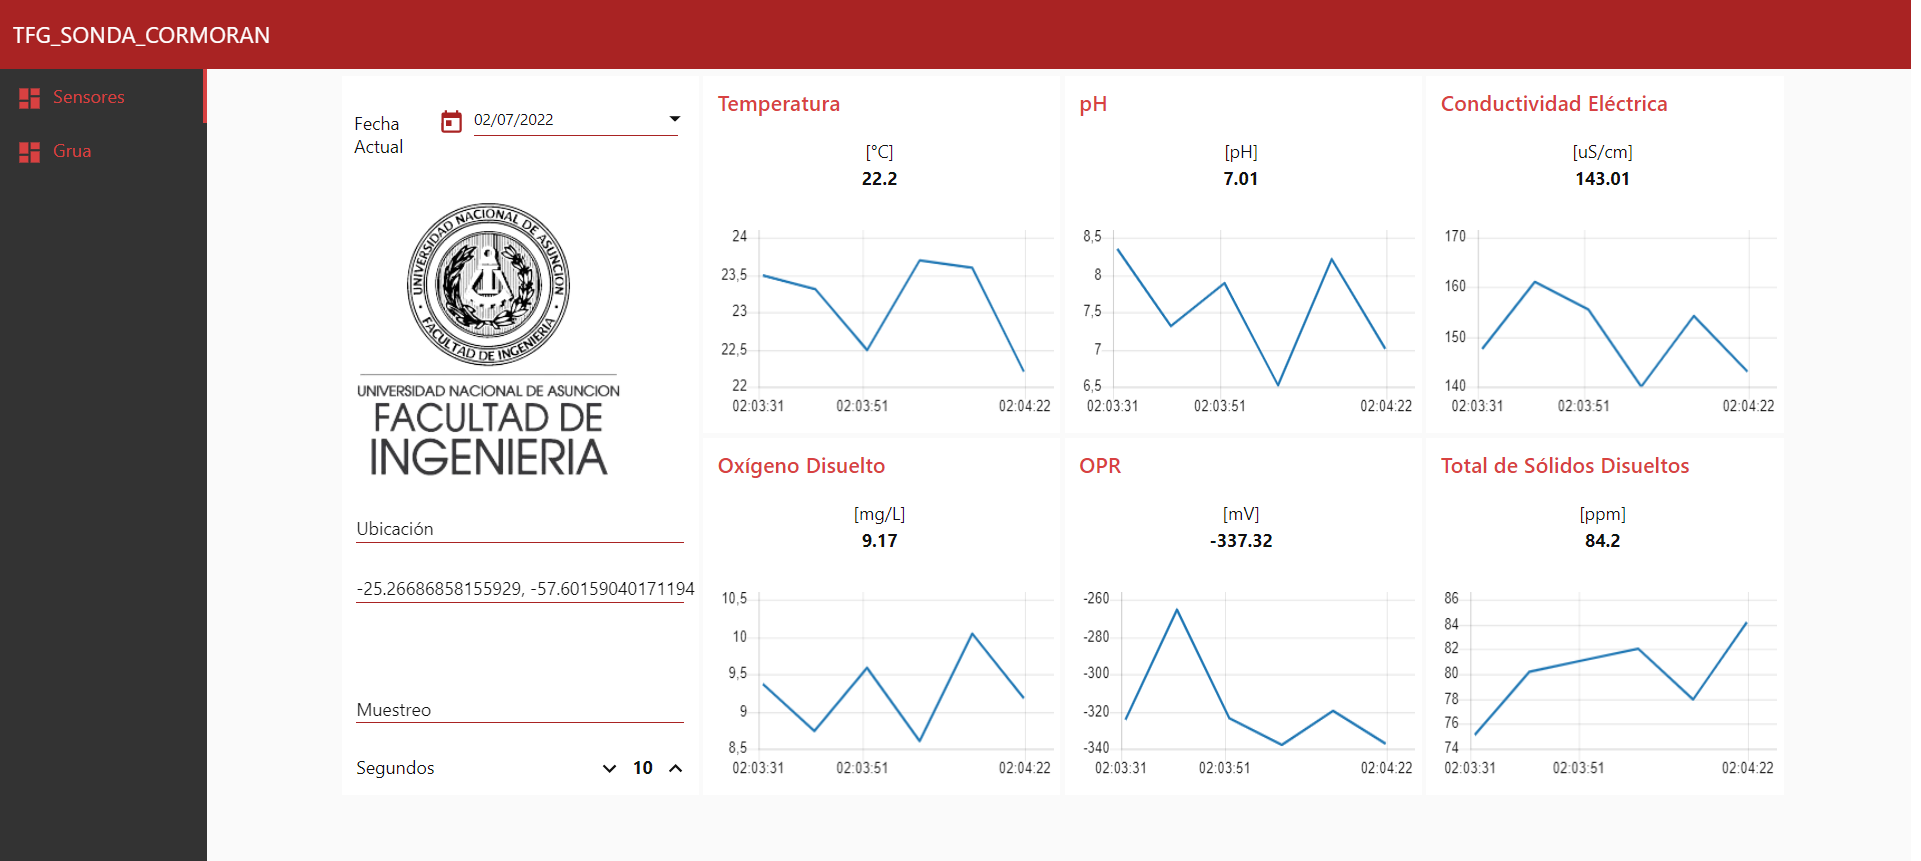
\includegraphics[scale=0.88]{Imagenes/cap4/nodeRed.png}
        \caption {Interfaz de monitoreo. }{\textbf{Fuente:}
        Elaboraci\'on Propia. }
        \label{fig:interfaz}
\end{figure}

Con la idea de conservar un dise\~no m\'inimo, se desarrollaron dos vistas principales. La primera vista, donde se pueda visualizar los datos recolectados por los sensores y otra vista para operaciones manuales. En la figura \ref{fig:interfaz} se puede apreciar el panel principal del monitoreo, donde se despliegan cada uno de los parámetros de temperatura, potencial de hidrógeno, conductividad eléctrica, oxigeno disuelto, potencial de oxigeno reducción y total de solidos disueltos, con gráficos obtenido de la representacion  con cada uno de los puntos obtenidos durante el muestreo de de la la sonda. Además se despliegan las informaci\'ones de la fecha, ubicación en coordenadas de latitud y longitud, del lugar donde se esta obteniendo cada una de las muestras.
\section[Presupuesto]{Presupuesto}
En la Tabla \ref{tab:presu} se puede apreciar los materiales utilizados en el presente TFG y los costos de los mismos.

\begin{table}[t]
\protect\caption{Presupuesto Final del TFG.}
     \label{tab:presu}
     \centering
\begin{tabular}{c l c c}
\hline
\multicolumn{4}{c}{\textbf{Parte mecánica}}\\ 
% \hline
\multicolumn{1}{c}{\textbf{Cant}}                 & 
\multicolumn{1}{c}{\textbf{Descripción}}           & 
\multicolumn{1}{c}{\textbf{Costo USD}}             & 
\multicolumn{1}{c}{\textbf{Total USD}} \\ 
\hline
\multicolumn{2}{l}{\textbf{Sonda}}                & 
\multicolumn{2}{l}{} \\ 
\hline
\multicolumn{1}{c}{1}                             & 
\multicolumn{1}{l}{Cilindro teflón sólido l x D 42x12 {[}cm {]}}        & 
\multicolumn{1}{r}{120,00}                            & 
\multicolumn{1}{r}{120,00}                \\ 
% \hline
\multicolumn{1}{c}{1}                             & 
\multicolumn{1}{l}{Soporte metálico}               & 
\multicolumn{1}{r}{5,00}                              & 
\multicolumn{1}{r}{5,00}                  \\ 
\multicolumn{1}{c}{1}                             & 
\multicolumn{1}{l}{Mecanizado}               & 
\multicolumn{1}{r}{100,00}                              & 
\multicolumn{1}{r}{100,00}                  \\ 
% \hline \\
\multicolumn{2}{l}{\textbf{Periféricos}}          & 
\multicolumn{2}{c}{}                                                             \\ 
\hline
\multicolumn{1}{c}{5}                              & 
\multicolumn{1}{l}{Caño PVC 3/8 pulg.}             & 
\multicolumn{1}{r}{2,00}                              & 
\multicolumn{1}{r}{10,00}                 \\ 
% \hline
\multicolumn{1}{c}{1}                             & 
\multicolumn{1}{l}{Soporte grúa}                   & 
\multicolumn{1}{r}{5,00}                              & 
\multicolumn{1}{r}{5,00}                  \\ 
% \hline
\multicolumn{2}{r}{\textbf{Total parte mecánica}} & 
\multicolumn{2}{r}{\textbf{USD 240,00}}                                             \\ 
\hline                                              &                                                                                                          &                                                                                                          &                                         \\  \\ 
\hline
\multicolumn{4}{c}{\textbf{Parte electrónica}}  \\
% \hline
\multicolumn{1}{r}{\textbf{Cant}}                 & 
\multicolumn{1}{c}{\textbf{Descripción}}           & 
\multicolumn{1}{c}{\textbf{Costo USD}}             & 
\multicolumn{1}{c}{\textbf{Total USD}} \\ 
\hline
\multicolumn{2}{l}{\textbf{Sonda}}                & 
\multicolumn{2}{c}{}                                                             \\ 
\hline
\multicolumn{1}{c}{1}                             & 
\multicolumn{1}{l}{Sensor pH de Atlas Scientific}  & 
\multicolumn{1}{r}{74,99}                          & 
\multicolumn{1}{r}{74,99}              \\ 
% \hline
\multicolumn{1}{c}{1}                             & 
\multicolumn{1}{l}{Sensor conductividad eléctrica Atlas Scient.} & 
\multicolumn{1}{r}{157,99}                         & 
\multicolumn{1}{r}{157,99}             \\ 
% \hline
\multicolumn{1}{c}{1}                             & 
\multicolumn{1}{l}{Sensor oxigeno disuelto de Atlas Scientific}    & 
\multicolumn{1}{r}{217,99}                         & 
\multicolumn{1}{r}{217,99}             \\ 
% \hline
\multicolumn{1}{c}{1}                             & 
\multicolumn{1}{l}{Sensor OPR de Atlas Scientific} & 
\multicolumn{1}{r}{114,99}                         & 
\multicolumn{1}{r}{114,99}             \\ 
% \hline
\multicolumn{1}{c}{1}                             & 
\multicolumn{1}{l}{Sensor temperatura}             & 
\multicolumn{1}{r}{11,95}                          & 
\multicolumn{1}{r}{11,95}              \\ 
% \hline
\multicolumn{1}{c}{1}                             & 
\multicolumn{1}{l}{Kit Raspberry pi 3 B+}          & 
\multicolumn{1}{r}{74,99}                          & 
\multicolumn{1}{r}{74,99}              \\ 
% \hline
\multicolumn{1}{c}{1}                             & 
\multicolumn{1}{l}{Tentacle Shield}                & 
\multicolumn{1}{r}{126,99}                         & 
\multicolumn{1}{r}{126,99}             \\ 
% \hline
\multicolumn{1}{c}{1}                             & 
\multicolumn{1}{l}{Driver pH de Atlas Scient.}     & 
\multicolumn{1}{r}{39,99}                          & 
\multicolumn{1}{r}{39,99}              \\ 
% \hline
\multicolumn{1}{c}{1}                             & 
\multicolumn{1}{l}{Driver conductividad eléctrica Atlas Scient.} & 
\multicolumn{1}{r}{59,99}                          & 
\multicolumn{1}{r}{59,99}              \\ 
% \hline
\multicolumn{1}{c}{1}                             & 
\multicolumn{1}{l}{Driver oxígeno disuelto de Atlas Scient.}        & 
\multicolumn{1}{r}{45,99}                          & 
\multicolumn{1}{r}{45,99}              \\ 
% \hline
\multicolumn{1}{c}{1}                             & 
\multicolumn{1}{l}{Driver OPR de Atlas Scientific} & 
\multicolumn{1}{r}{39,99}                          & 
\multicolumn{1}{r}{39,99}              \\ 
% \hline
\multicolumn{1}{c}{1}                             & 
\multicolumn{1}{l}{Batería LiPo nano-tech 5100mAh} & 
\multicolumn{1}{r}{41,93}                          & 
\multicolumn{1}{r}{41,93}              \\ 
% \hline
\multicolumn{1}{c}{1}                             & 
\multicolumn{1}{l}{Conversor DC-DC}                & 
\multicolumn{1}{r}{10,00}                             & 
\multicolumn{1}{r}{10,00}                 \\ 
% \hline
\multicolumn{1}{c}{1}                             & 
\multicolumn{1}{l}{PCB}                            & 
\multicolumn{1}{r}{20,00}                             &
\multicolumn{1}{r}{20,00}                 \\ 
% \hline\\
\multicolumn{2}{l}{\textbf{Periféricos}}          &
\multicolumn{2}{l}{}                                                             \\ 
\hline
\multicolumn{1}{c}{2}                             & 
\multicolumn{1}{l}{NodeMCU}                        & 
\multicolumn{1}{r}{12,00}                             & 
\multicolumn{1}{r}{24,00}                 \\ 
% \hline
\multicolumn{1}{c}{1}                             & 
\multicolumn{1}{l}{Sonar ultrasónico}              & 
\multicolumn{1}{r}{89,95}                          & 
\multicolumn{1}{r}{89,95}              \\ 
% \hline
\multicolumn{1}{c}{4}                             & 
\multicolumn{1}{l}{Bateria Ion litio 2000mAh}      & 
\multicolumn{1}{r}{12,95}                          & 
\multicolumn{1}{r}{51,8}               \\ 
% \hline
\multicolumn{1}{c}{1}                             & 
\multicolumn{1}{l}{Cabrestante eléctrico}          & 
\multicolumn{1}{r}{119,75}                         & 
\multicolumn{1}{r}{119,75}             \\ 
% \hline
\multicolumn{1}{c}{1}                             & 
\multicolumn{1}{l}{Driver de motor bidireccional}  & 
\multicolumn{1}{r}{29,99}                          & 
\multicolumn{1}{r}{29,99}              \\ 
\hline 
\multicolumn{2}{r}{\textbf{Total parte electrónica }}  & 
\multicolumn{2}{r}{\textbf{USD 1.353,27}}   \\ 
% \hline
\multicolumn{2}{r}{\textbf{Mano de obra}}         & 
\multicolumn{2}{r}{\textbf{ USD 2.200,00}}      \\ 
% \hline
\multicolumn{2}{r}{\textbf{Total genera}}        & 
\multicolumn{2}{r}{\textbf{USD 3.793,27}}  \\ 
\hline
\end{tabular}
\end{table}
     \chapter[Capítulo 5. Conclusi\'on y Trabajos Futuros]{ Conclusión y Trabajos Futuros}
\pagestyle{fancy}



Se logro dise\~nar un sonda con la capacidad de alojamiento de los sensores de conductividad el\'ectrica, potencial de hidr\'ogeno, oxigeno disuelto, potencial de oxigeno reducci\'on, temperatura, salinidad, y componentes elect\'onicos .
Empleando t\'ecnicas de mecanizado, se logro fabricar la sonda en material de nylon.
Se logro dotar de funcionalidad para medici\'on a multinivel mediante el uso motores el\'ectricos y con control programable del usuario.
Se logro implementar con la herramienta nodeRed una interfaz visual gr\'afica, que despliegue toda la informaci\'on de los sensores y f\'acil e intuitiva.
Se efectuaron varias pruebas de campo en el lago Ypakarai, laguna Pyta, laboratorio sistemas distribuidos y laboratorios de qu\'imica FIUNA. 
    %  \chapter[Capítulo 6. ]{}
\pagestyle{fancy}

% %%%%%%%%%%%%%%%%%% CAPITULO AUXILIAR 

Borrador

El t/'ermino humedal incluye todos los cuerpos de agua l/'enticos poco profundos, temporales o permanentes, donde la luz llega al fondo permitiendo el desarrollo.\cite{quintana_new_2016} 


%% Calidad de Ahuas
En el 


\begin{table}[]
\begin{tabular}{|l|ccc|ccc}
\hline
Muestra 2                                                                       & \multicolumn{3}{c|}{LSD}                                                                                                                                 & \multicolumn{3}{c|}{QCA}                                                                                                                                                     \\ \hline
\textbf{\begin{tabular}[c]{@{}l@{}}Análisis de datos \\ obtenidos\end{tabular}} & \multicolumn{1}{c|}{\begin{tabular}[c]{@{}c@{}}T \\ °C\end{tabular}} & \multicolumn{1}{c|}{pH}      & \begin{tabular}[c]{@{}c@{}}CE\\ $\mu S/cm$\end{tabular} & \multicolumn{1}{c|}{\begin{tabular}[c]{@{}c@{}}T \\ °C\end{tabular}} & \multicolumn{1}{c|}{pH}     & \multicolumn{1}{c|}{\begin{tabular}[c]{@{}c@{}}CE\\ $\mu S/cm$\end{tabular}} \\ \hline
Desviación Estandar                                                             & \multicolumn{1}{c|}{0.291}                                           & \multicolumn{1}{c|}{0.165}   & 3.545                                              & \multicolumn{1}{c|}{0.354}                                           & \multicolumn{1}{c|}{0.167}  & \multicolumn{1}{c|}{1.125}                                              \\ \hline
Varianza                                                                        & \multicolumn{1}{c|}{0.0845}                                          & \multicolumn{1}{c|}{0.027}   & 12.57                                              & \multicolumn{1}{c|}{0.125}                                           & \multicolumn{1}{c|}{0.0279} & \multicolumn{1}{c|}{1.267}                                              \\ \hline
\begin{tabular}[c]{@{}l@{}}Coeficiente de \\ Variación\end{tabular}             & \multicolumn{1}{c|}{1.287}                                           & \multicolumn{1}{c|}{2.616}   & 9.816                                              & \multicolumn{1}{c|}{1.582}                                           & \multicolumn{1}{c|}{2.379}  & \multicolumn{1}{c|}{2.201}                                              \\ \hline
Error Estándar                                                                  & \multicolumn{1}{c|}{0.075}                                           & \multicolumn{1}{c|}{0.0426}  & 0.915                                              & \multicolumn{1}{c|}{0.0914}                                          & \multicolumn{1}{c|}{0.043}  & \multicolumn{1}{c|}{0.290}                                              \\ \hline
Covarianza                                                                      & \multicolumn{1}{c|}{0.0564}                                          & \multicolumn{1}{c|}{-0.351}  & 0.157                                              &                                                                      &                             &                                                                         \\ \cline{1-4}
Correlación                                                                     & \multicolumn{1}{c|}{0.5483}                                          & \multicolumn{1}{c|}{-0.0096} & 0.628                                              &                                                                      &                             &                                                                         \\ \cline{1-4}
\end{tabular}
\end{table}







\begin{table}[]
\begin{tabular}{clll}
\hline
\textbf{Sector}                                                         & \multicolumn{1}{c}{\textbf{Actividad}}                                                      & \multicolumn{1}{c}{\textbf{Efectos}}                                                                 & \multicolumn{1}{c}{\textbf{Área}}                                                                        \\ \hline
\multirow{6}{*}{\begin{tabular}[c]{@{}c@{}}Centro\\ Oeste\end{tabular}} & Urbana e industrial                                                                         & \begin{tabular}[c]{@{}l@{}}Contaminación superficial y \\ \\ acuíferos.\end{tabular}                 & \begin{tabular}[c]{@{}l@{}}REMA (Región Metropolitana \\ de Asunción)\\ Cuenca de Ypacarai.\end{tabular} \\
                                                                        & Mataderos y frigoríficos                                                                    & Aguas superficiales                                                                                  & REMA                                                                                                     \\
                                                                        & \multirow{2}{*}{\begin{tabular}[c]{@{}l@{}}Expansión Urbana \\ \\ desordenada\end{tabular}} & Destrucción de fuentes de agua                                                                       & \begin{tabular}[c]{@{}l@{}}Cuenca de Ypacarai\\ Cuenca del Ypoa\end{tabular}                             \\
                                                                        &                                                                                             & Aguas superficiales                                                                                  & REMA                                                                                                     \\
                                                                        & \begin{tabular}[c]{@{}l@{}}Cementera\\ Metalurgica\end{tabular}                             & \begin{tabular}[c]{@{}l@{}}Contaminación superficial y \\ \\ acuíferos\end{tabular}                  & \begin{tabular}[c]{@{}l@{}}REMA\\ Villa Hayes\end{tabular}                                               \\
                                                                        & Prácticas agrícolas .                                                                       & \begin{tabular}[c]{@{}l@{}}Colmatación por erosión y \\ \\ contaminación por pesticidas\end{tabular} & Todos los Deptos                                                                                         \\ \cline{2-4} 
\end{tabular}
\hfill \textbf{Fuente:} Extra\'ido de \cite{salas-duenas-2015}.
\end{table}





%%%%%%%%%%%%%%%%%%%%%%%%%%%%%%CAP 3


\subsection{}section[Descripción General del Sistema]{Descripción General del Sistema}

El modelo del sistema, está compuesto por varios subsistemas o bloques escalables, independientes y que se pueden comunican entre s\'i, mediante un un intermediario que se encarga de coordinar los datos entre los distintos bloques. El sistema general se podr\'ia dividir en tres segmentos principales, por un lado el subsistema central \textit{la sonda}, de mayor complejidad que se encarga de recepci\'on y transmisi\'on de datos y nexo con los otros subsistemas, ejecuta el muestreo con los sensores, almacena en una base local los datos, la \textit{estacion remota}, la sala de monitoreo donde se puede visualizar los datos recibido de la sonda y realizar configuraciones de muestreo, los subsistemas menos complejos se denominar perif\'ericos, son bloques auxiliares escalables en medida que sean necesarios, y de esa forma aumentar las funcionalidades del sistema, en el presente TFG de desarrollaron e implementaron los perif\'ericos que ayuden para el muestreo a multiniveles como ser perif\'ericos de \textit{batimetr\'ia}, para conocer la profundidad del lugar de muestreo y perif\'erico de \textit{gr\'ua} que le otorga a la sonda la posibilidad de desplazamiento vertical para pueda tomar muestras a multiniveles y el perif\'erico \textit{ASV}, provee la ubicaci\'on georeferenciada del punto de muestreo y otorga a la sonda la posibilidad de desplazamiento horizontal sobre toda la superficie a ser analizada. Los modos de operaci\'on pueden ser autom\'aticos, donde ejecuta un algoritmo en sincron\'ia con el ASV o manual donde el usuario desde la estaci\'on remota puede configurar los par\'ametros que requiera.  
El diagrama de funcionamiento del sistema se pude apreciar en la Figura \ref{fig:3.1}.

%%%%https://es.overleaf.com/project/5ca9254d2df4572fd3ca381a
asd 


\subsubsection{Sonda}








\section{Aspectos Generales}
El desarrollo de la sonda implic\'o una serie de desaf\'ios t\'ecnicos, por ese motivo esa secci\'on se organiza de la siguiente manera

\begin{itemize}
    \item Dise\~no Mec\'anico: abarca todos los criterios considerados al dise\~no de la sonda y sistema de despliegue. 
    \item Fabricaci\'on Mec\'anica: abarca las t\'ecnicas y materiales empleadas para la fabricaci\'on de los componentes.
    \item Programaci\'on e Integraci\'on de los sensores: en esta secci\'on abarca lo referente a los distintos script desarrollados para lograr el funcionamiento del dispositivo.
\end{itemize}
\section{Dise\~no Mec\'anico}
Para el proceso de dise\~no se siguieron los procedimientos de XXX donde agrupan el proceso de dise\~no en las siguientes etapas:
Etapas del dise\~no: 

\subsection{Sonda}
\subsubsection{Conceptualizaci\'on}
Conceptualmente se definen los requerimientos m\'inimos para el correcto funcionamiento de la sonda.
\begin{itemize}
    \item versatilidad: su implementación debe de ser independiente a la dispositivo de soporte, pudiendo operar en cualquier medio de transporte.
    \item 
    \item Energ\'ia: la donde deber\'a tener autonom\'ia energ\'etica para sus operaciones de monitoreo,  
\end{itemize}
la donde deberá de contener en su interior al menos cinco sensores  (ph,CE,OD,OPR,T), adem\'as de toda la electr\'onica necesaria para la operaci\'on de estos. La sonda deber\'a tener autonom\'ia energ\'etica y poder sumergirse hasta una profundidad m\'inima de 5 metros , teniendo en cuenta que la profundidad promedio del lago Ypakarai es de 3 metros [\cite{hidrologiaItaipu}].
   
\subsubsection{An\'alisis}
En base a las conceptualizaci\'on de la secci\'on aterior y los materiales disponibles en el pa\'is se concluyen  :


\subsection{Despliegue}
\subsubsection{Conceptualizaci\'on}

deber\'a brindar soporte para que la sonda pueda hacer mediciones a varios niveles, dise\~no simple y adaptativo para ser instalado en embarcaciones de investigaci\'on.

\subsubsection{An\'alisis}
En base a las conceptualizaci\'on de la secci\'on aterior y los materiales dispobibles en el pa\'is se concluyen  :
\begin{itemize}
    \item Sonda: .
    \item Despliegue: deber\'a brindar soporte para que la sonda pueda hacer mediciones a varios niveles, dise\~no simple y adaptativo para ser instalado en embarcaciones de investigaci\'on.
\end{itemize}

\subsection{Diseño, Mecanizado de Piezas}



\section{Fabricaci\'on}





%-----------------------------------------------------------------------------




         

\subsection{Referencias Comerciales.}
Las pocas empresas que se dedican al rubro de la construcción de invernaderos Hidropónicos, las que se dedican al riego automatizado o las de ferti-riego ofrecen soluciones a proyectos de gran envergadura, debiéndose especificar siempre las hectáreas de plantación que se desean controlar para que tomen en cuenta el proyecto, lo diseñen y así puedan enviar un presupuesto al cliente interesado.
Según revisión de existencia local no existe un producto comercial del tipo de este trabajo dentro del territorio paraguayo.\textbf{}





%%%%%%%%%%%%%%%%%%%%%%%%%%%%%%%%%%%%%%%%%%%%%%%%%%%%%%%%%%%%%%%%%%%%%%%%%%%%%%%%%%%%%%%%%%%%%%%%
%%%%%%%%%%%%%%%%%%%% ANOTADOR CAP 1 %%%%%%%%%%%%%%%%%%%%%%%%%%%%%%%%%%

Monitoreo del agua potable: los parámetros químicos comunes incluyen pH, nitratos y oxígeno disuelto. 

La medición de O2 (o DO) es un indicador importante de la calidad del agua. 
Los cambios en los niveles de oxígeno disuelto indican la presencia de microorganismos de aguas residuales, escorrentías urbanas o agrícolas o descargas de fábricas. 

Un nivel adecuado de ORP minimiza la presencia de microorganismos como  E. coli, Salmonella, Listeria . 

Los niveles de turbidez por debajo de 1 NTU indican la pureza adecuada del agua potable.

Detección de fugas químicas en ríos : pH extremo o valores bajos de OD indican derrames químicos debido a problemas en la planta de tratamiento de aguas residuales o en la tubería de suministro.

Medición remota de piscinas : la medición del potencial de oxidación-reducción (ORP), el pH y los niveles de cloro del agua puede determinar si la calidad del agua en piscinas y spas es suficiente para fines recreativos.

Niveles de contaminación en el mar : la medición de los niveles de temperatura, salinidad, pH, oxígeno y nitratos proporciona información para los sistemas de detección de calidad en el agua de mar.

Prevención de la corrosión y depósitos de cal:  Controlando la dureza del agua podemos evitar la corrosión y depósitos de cal en lavavajillas y dispositivos de tratamiento de agua como calentadores. 

La dureza del agua depende de: pH, temperatura, conductividad y concentraciones de calcio (Ca + ) / magnesio (Mg 2+ ).

Cultivo de abetos / Monitoreo de tanques de peces / Criadero / Acuicultura / Acuaponía: Medición de las condiciones del agua de animales acuáticos como caracoles, peces, cangrejos de río, camarones o langostinos en tanques. 

Los valores importantes son el pH, el oxígeno disuelto (DO), el amoníaco (NH 4 ), el nitrato (NO 3 - ), el nitrito (NO 2 - ) y la temperatura del agua.

Hidroponía : las plantas que toman los nutrientes directamente del agua necesitan un pH preciso y niveles de oxígeno en el agua (OD) para obtener el máximo crecimiento.

Las sondas del sensor miden más de 12 parámetros químicos y físicos de la calidad del agua, como pH, nitratos (NO3), iones disueltos (fluoruro (F - ), calcio (Ca 2+ ), nitrato (NO 3 - ), cloruro (Cl - ), Yoduro (I - ), Cúprico (Cu 2+ ), Bromuro (Br - ), Plata (Ag + ), Fluoroborato (BF 4 - ), Amoníaco (NH 4 ), Litio (Li + ), Magnesio (Mg 2+ ) , Nitrito (NO 2- ), Perclorato (ClO 4 ), Potasio (K + ), Sodio (Na +) oxígeno disuelto (OD), conductividad (salinidad), potencial de oxidación-reducción (ORP), turbidez, temperatura, etc.

Los contaminantes pueden detectarse y tratarse en tiempo real para garantizar una buena calidad del agua en toda la red de suministro de agua. 
Los valores extremos de pH pueden indicar derrames de productos químicos, problemas en la planta de tratamiento o problemas en las tuberías de suministro. 
Los niveles bajos de OD pueden indicar la presencia de microorganismos debido a escorrentías urbanas / agrícolas o derrames de aguas residuales. 
El ORP mide qué tan bien está funcionando la desinfección del agua.






%%%%%%%%%%%%%%%%%%%%%%%%%%%%%%%%%%%%%%%%%%%%%%%%%%%%%%%%%%%%%%%%%%%%%%%%%%%%%%%%%%%%%%%%%%%%%%%%%%%%%%%%%%%%%%%%%%%%%%%%%%


%Desde acá considerar pasar todo al cap 3
\section{T\'ecnicas de fabricaci\'on mecanicas}
% http://www.scielo.org.co/scielo.php?script=sci_arttext&pid=S0120-56092006000300014
% https://books.google.com.co/books?id=tcV0l37tUr0C&printsec=frontcover#v=onepage&q&f=false
% http://ve.scielo.org/scielo.php?script=sci_arttext&pid=S1316-48212014000400003
% https://www.3dnatives.com/es/los-mejores-libros-impresion-3d-22042016/#!
% https://es.wikipedia.org/wiki/Impresi%C3%B3n_3D
% https://esvigrocircuitos.webnode.mx/_files/200000118-58b4259ae5/Identificaci%C3%B3n%20general%20de%20sistemas%20y%20t%C3%A9cnicas%20de%20fabricaci%C3%B3n.pdf
% % https://www.redalyc.org/jatsRepo/944/94454631006/html/index.html
% https://books.google.com.py/books?id=gBuyDwAAQBAJ&printsec=frontcover&dq=impresion+3D&hl=es-419&sa=X&redir_esc=y#v=onepage&q&f=false
% https://books.google.com.py/books?id=JQ9djwEACAAJ&dq=impresion+3D&hl=es-419&sa=X&redir_esc=y
% https://books.google.com.py/books?id=fvJ9DwAAQBAJ&pg=PT8&dq=impresion+3D&hl=es-419&sa=X&ved=2ahUKEwi5ptXwte33AhXhmZUCHZgHD3wQ6AF6BAgHEAI#v=onepage&q=impresion%203D&f=false

\section{Dise~/no de interfaz}
% https://nodered.org/
% https://docs.python.org/3/library/tkinter.html

\section{Base de Datos}
% % https://www.oracle.com/mx/database/what-is-database/
% https://www.postgresql.org/
% https://www.sqlite.org/index.html
% https://books.google.com.py/books?id=HmnHeZ1wsvwC&printsec=frontcover&dq=bases+de+datos&hl=es-419&sa=X&redir_esc=y#v=onepage&q=bases%20de%20datos&f=false
% https://books.google.com.py/books?id=EwcuBwAAQBAJ&printsec=frontcover&dq=bases+de+datos&hl=es-419&sa=X&redir_esc=y#v=onepage&q=bases%20de%20datos&f=false
% https://books.google.com.py/books?id=LDOGzQEACAAJ&dq=bases+de+datos+sqlite&hl=es-419&sa=X&redir_esc=y

\section{Comunicaci\'on}
% https://mecatronicaexperimental.weebly.com/protocolos-de-comunicacioacuten.html
% https://sites.google.com/site/protocolosse/
% https://cs.uns.edu.ar/materias/se/2019/descargas/teoria/clase08-comunicacion-slides.pdf
% https://www.virtual-serial-port.org/es/articles/serial-communication-in-embedded-development/
% https://1library.co/article/protocolos-de-comunicaci%C3%B3n-en-sistemas-embebidos.zlnpvxrq
% http://sedici.unlp.edu.ar/bitstream/handle/10915/72131/Tesis.%20Protocolos%20de%20comunicaci%C3%B3n%20entre%20microcontroladores.pdf-PDFA.pdf?sequence=2&isAllowed=y
% https://books.google.com.py/books?id=5gSQhn0LCOsC&pg=PA117&dq=1wire&hl=es-419&sa=X&ved=2ahUKEwiT8ey9te33AhVeI7kGHcCbCXUQ6AF6BAgKEAI#v=onepage&q=1wire&f=false
% https://books.google.com.py/books?id=aGVTAAAAMAAJ&q=i2c&dq=i2c&hl=es-419&sa=X&ved=2ahUKEwjissm4te33AhV_BLkGHTVsC3kQ6AF6BAgJEAI


%%%%%%%%%%%%%%%%%%%%%%%%%%%%%%%%%%%%%%




    %%%bibliografía%%%%%%%%%
    %Cargar los libros en formato bibtex en el archivo fiuna.bib
    \formatoIndice
    \bibliographystyle{fiuna}
    % \bibliographystyle{report}

    \nocite{*}
    %%%\bibliography{fiuna}   
    \bibliography{fiuna.bib}
    
    %%%anexos%%%%%%
    %En caso de no tenerlos, comentar la siguiente línea
    \appendixpageoff
\begin{appendices}
%Agregar los apéndices

%\chapter*{Anexo A}
%\addcontentsline{loa}{appendix}{Anexo A: Titulo del anexo A}

%Aquí el contenido del anexo A

%\chapter*{Anexo B: El uso de plantillas}
%\addcontentsline{loa}{appendix}{Anexo B: El uso de plantillas}

%Aquí el contenido del anexo B
\chapter*{Anexo A}
\addcontentsline{loa}{appendix}{Anexo A: Mapas}

\begin{figure}[ht]
    \centering
    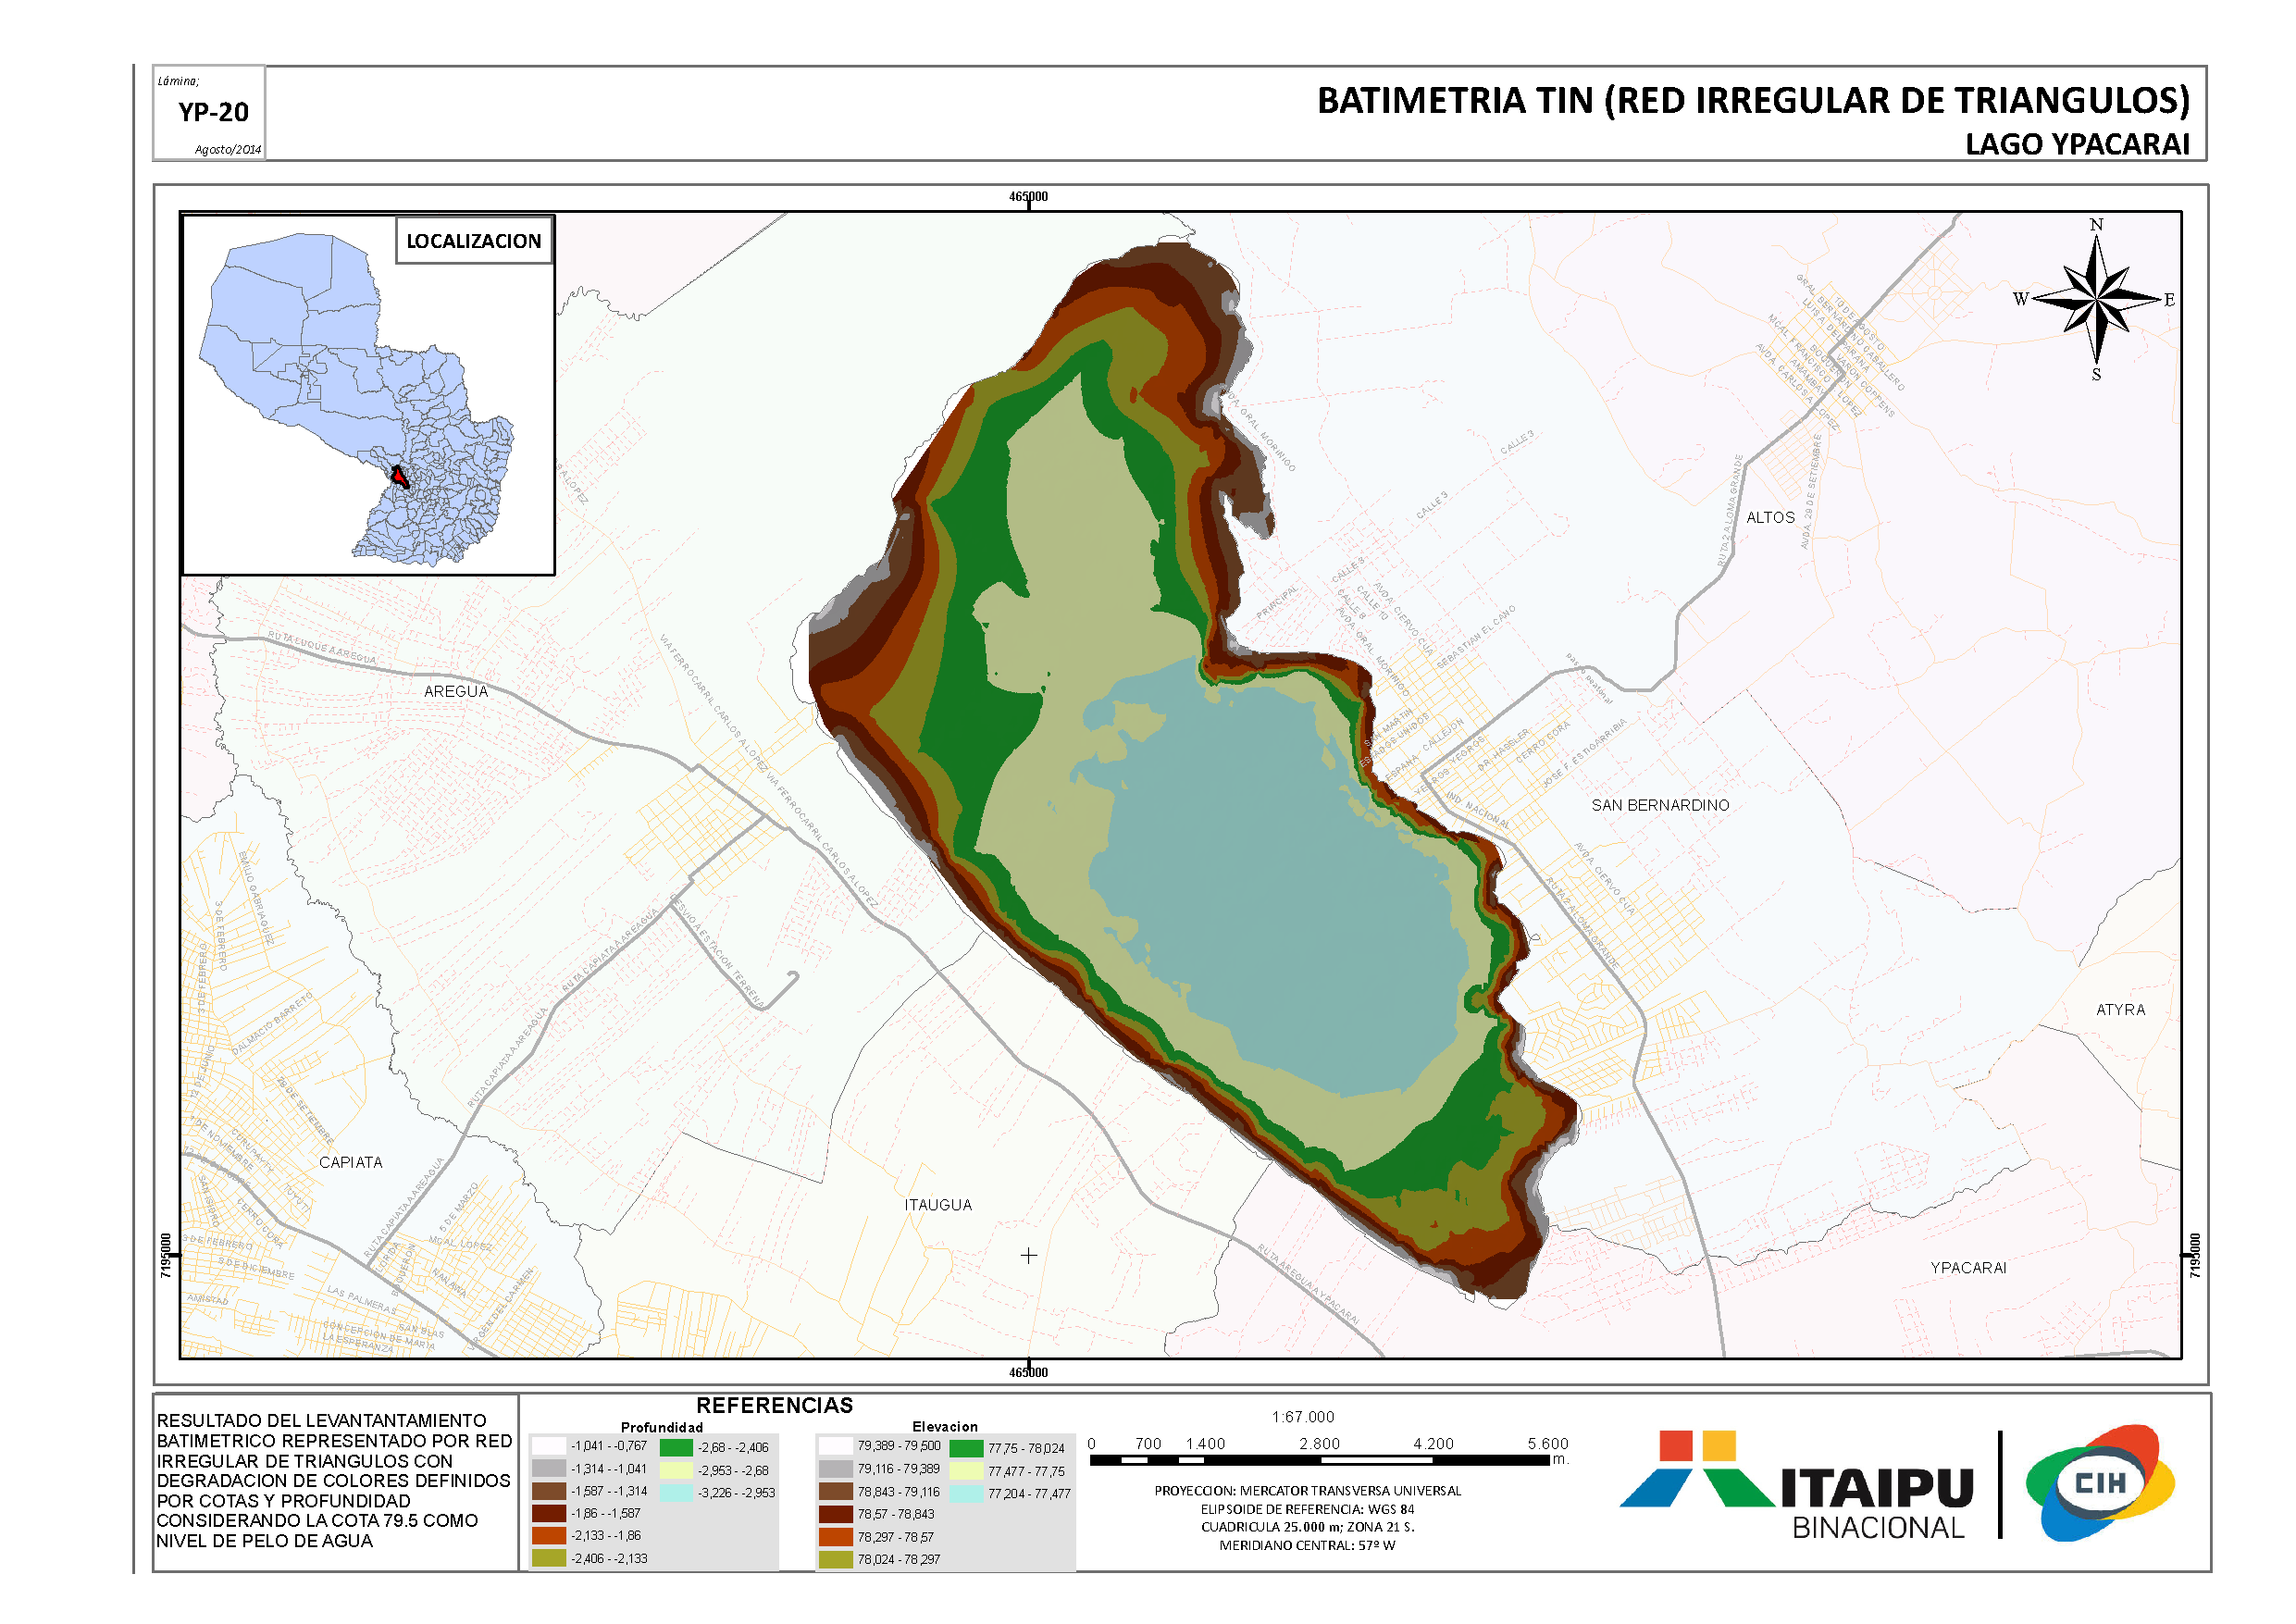
\includegraphics[width=150mm, height=100mm]{Imagenes/cap3/Batimetria_lago_Ypacarai_TIN_A3.pdf}
    \caption[BATIMETRIA TIN lago Ypakarai]{Batimetr\'ia TIN (RED IRREGULAR DE TRIANGULOS), lago Ypakarai} \textbf{Fuente:  Itaipu Binacional.}
    \label{fig:BatimetriaItaipu}
\end{figure}

\chapter*{Anexo B: Cormor\'an - I}
\addcontentsline{loa}{appendix}{Anexo B: Cormor\'an -I }
\label{Anexo:Cormoran}
El diseño final de la sonda, fue el resultado de varias versio7777777777nes que fueron modificándose de tal manera que resulte mejor y se adapte a los requerimientos del proyecto.
Partiendo de un diseño de un misil militar por su dise\~no din\'amico , similar al propuesto por [1], modificado hasta la versión final con el cual se realizaron las pruebas. Su diseño modular esta pensado para el caso que se le requiera sacar o añadir uno o mas sensores, se pueda seguir utilizando la sonda con cambios mínimos para adaptación.
La primera sonda fue impresa en su totalidad con una impresora 3D, en material Acrilonitrilo butadieno Estireno(ABS), por sus propiedades de alta resistencia al impacto y su baja degradación en presencia de líquidos. 
El diseño de la sonda (Sonda V4.3) utilizado en el Cormoran-I, esta disen\~ado para ser albergar a seis sensores específicos de la empresa Atlas Scientific.

\begin{itemize}
    \item Sonda PH de Plata/cloruro de plata de calidad científica, EZO pH Circuit.
    \item Sonda ORP de barra de platino, EZO OPR Circuit.
    \item Sonda de conductividad: 5 [\(\mu S/cm\)] a 200,000 [\(\mu S/cm\)], EZO Conductivity Circuit.
    \item EZO RGB, Sensor de color integrado 8bit.
    \item Sonda de oxígeno disuelto, EZO OD Circuit.
    \item Sensor de Temperatura DS18B20. Sparkfun.
\end{itemize}
    
\subsection{Versiones de la Sonda }
Se desarrollaron cuatro versiones de la sonda, con el programa de diseño CAD 3D SolidWorks 2015. La sonda es un un ensamble de tres piezas principales, denominadas:

\begin{itemize}
\item \textbf{Frente} : Pieza frontal de la sonda, la función de esta pieza es principalmente de protección contra basura o objetos que puedan dañar a los sensores. Se dise\~no de forma cil\'indrica hueca de base circular para las versiones de la sonda Figura1-a y Figura1-b, las de base elipsoidal para las versiones Figura1-d y Figura1-e, Posee ranuras laterales para que el agua ingrese dentro de la cavidad hueca de esta pieza y los sensores puedan hacer las mediciones.  
\item \textbf{Anillo} : Pieza central de la sonda y enlace de las otras dos piezas, la función de esta pieza es servir de soporte a las sensores y posicionarlos de forma horizontal. En el caso que se requiera otros sensores, esta es la única pieza que tendría que ser adaptado a los nuevos sensores.
\item \textbf{Base}  : Pieza posterior de la sonda, su función es de protección de los cables de los sensores. 
\end{itemize}

\begin{enumerate}
\item \textbf{Sonda V0.0:} La versión inicial de la sonda, con diseño cilíndrico de base circular, el inconveniente principal de este diseño fue la debilidad estructural de la parte frontal de la sonda por la cantidad de ranuras, ademas el diseño de la punta dificultaba bastante para ser impreso en la impresora 3D.
\begin{figure}[ht]
    \centering
    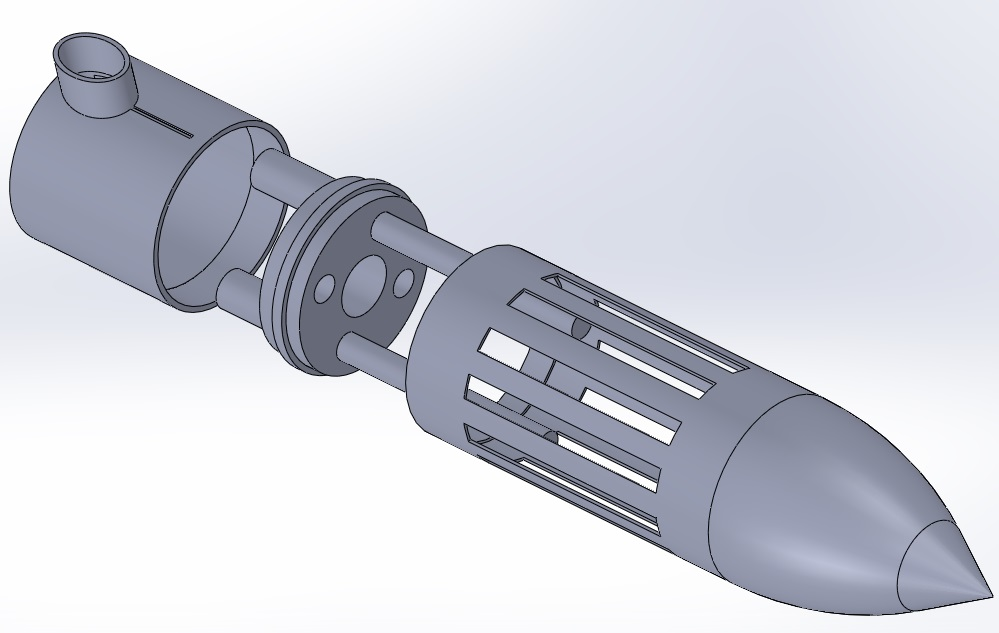
\includegraphics[width=50mm]{Imagenes/Sonda_v0.jpg}
    \caption{Caption}
    \label{fig:my_label}
\end{figure}

\item \textbf{Sonda V1.0:} La siguiente versión, resolvía los problemas de debilidad estructural de la parte frontal espaciando mas las ranuras y reemplazando la punta de la pieza frontal con un diseño mas redondeado para que pueda ser impresa con mayor facilidad.   
\item \textbf{Sonda V2.0:} En esta versión de la sonda, se probaron con otras geometrías para mejorar la dinámica del fluido, de esta forma cargar menos al motor propulsor del Dron. El inconveniente de este diseño fue, que por su geometría era mas grande que el anterior por tanto utilizaba mas material.
\item \textbf{Sonda V3.0:} La siguiente versión se opto por una base elipsoidal para la sonda, ademas se agrego al diseño un soporte para que pueda ser fijado al Dron con tornillos en la parte inferior, se realizaron cambios en la base para crear un ensamble mas dinámico. Fue la primera aproximación para el diseño final, el inconveniente de esta sonda era el soporte que resultaba poco practico de implementar y podría causar daños estructurales al casco del dron.
\item \textbf{Sonda V4.0:} La ultima versión resuelve el problemas de soporte, al agregar un riel en la parte superior de toda la sonda para fijarlo cuando se requiera al dron sin la utilización de tornillos o algún elemento fijador que pueda dañar el casco del dron.
\item \textbf{Sonda V4.1:} En la primera modificación de la versión 4 de la sonda, se optimizo el tamaño de la pieza frontal de la sonda,  para utilizar menos material y ofrecer mayor protección a las puntas de los sensores.
\item \textbf{Sonda V4.2:} En la segunda revisión de la versión 4, se re diseño la parte posterior de la sonda, para reemplazar el sistema modo inicial que conectar los sensores al dron, que en las versiones anteriores se encontraba en la parte superior, y como esta versión se diseña el riel, se opto por hacer por una perforación e la base para que por ella pueda conectarse al Dron.
\item \textbf{Sonda V4.3:} En la ultima revisión de la versión 4, se re diseña la pieza central de la sonda para agregarle un juego de juntas de gomas circulares, por los agujeros preparados para los sensores para de esta forma ejercer sobre ellos un mejor agarre, ademas se modifica la dimensión de sensor ubicado en la parte central de la pieza.
\end{enumerate}


\begin{figure}[htbp]
    \centering
 %   \subfigure[V0.0]{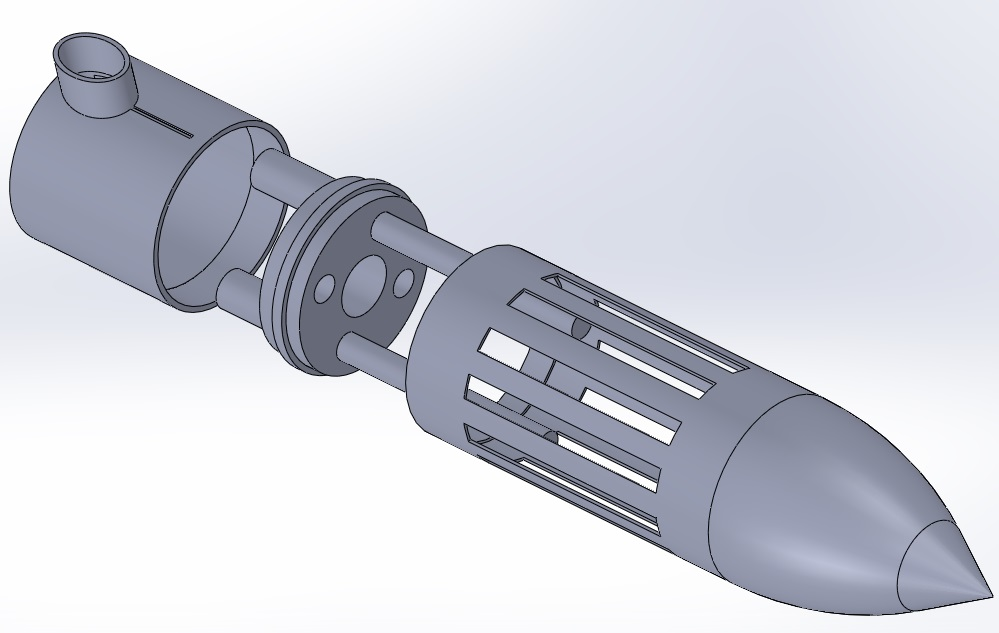
\includegraphics[width=50mm]{Imagenes/Sonda_v0.jpg}}
    
 %   \subfigure[V1.0]{\includegraphics[width=50mm]{Imagenes/Sonda_v1.jpg}}
    
%    \subfigure[V2.0]{\includegraphics[width=50mm]{Imagenes/Sonda_v2.jpg}}
    
  %  \subfigure[V3.0]{\includegraphics[width=50mm]{Imagenes/Sonda_v3.jpg}}
    
  %  \subfigure[V4.0]{\includegraphics[width=50mm]{Imagenes/Sonda_v4.jpg}}
    
    \caption{Versiones Sonda. Fuente: elaboración propia} \label{fig:Sonda_Versiones1}
    \end{figure}
    
    \begin{figure}[htbp]
    \centering
%\subfigure[V4.3 . Frontal]{\includegraphics[width=40mm]{Imagenes/Sonda_v4_1.jpg}}
    
%    \subfigure[V4.3 . Anillo]{\includegraphics[width=40mm]{Imagenes/Sonda_v4_2.jpg}}
    
%    \subfigure[V4.3 . Base]{\includegraphics[width=40mm]{Imagenes/Sonda_v4_3.jpg}}
    
    \caption{Versiones Sonda. Fuente: elaboración propia} \label{fig:Sonda_Versiones2}
\end{figure}

\section{Sonda v5.0}
Para el proyecto PINV15-177, se deberán realizar una serie de cambios al modelo final de la sonda utilizado en el CORMORAN-I, por la operación a multivinel, el material a ser utilizado y la ubicación de la electrónica.
\subsection{Operación Multinivel}
Como se introduce la capacidad de poder censar a multiniveles, es necesario cambiar el tipo de material de construcción para que de esta forma se pueda sumergir con su propio peso, y no requiera de otro medio externo para sumergirse. 
\subsection{Sonda Embebida}
Considerando que la versión 4.3, la sonda se fija por el casco del dron, el circuito de control y la base de datos se ubica dentro del dron, y los sensores de la sonda se conectan mediante cables coaxiales, segun datos proveídos por el informe de batimetria, realizado en el agosto del 2014  por la Dirección de Coordinación Ejecutiva del Centro Internacional de Hidroinformatica (CIH) dependiente de la Hidroeléctrica Itaipu, la máxima profundidad del lago Ypakarai es de 3,226[m], para la operación multinivel para estas profundidades la implementacion de versión actual resulta poco practica ya que se requerirán cables mas largos, expuestos al ambiente, agua, tracción pudiendo dañarse o registrar lecturas erróneas.\\ Para subsanar este inconveniente se propone que todo la electrónica se encuentre dentro de la sonda, en la parte posterior o base, de esta forma ademas eliminar el uso de cables, la sonda por si sola ya sera capaz de operar.

\subsection{Primera Versi\'on sonda Embebida}

\subsection{Diseño - Modelado}
El dise\~no y modelado de la sonda se realizo, utilizando el software de modelacion 3D SolidWorks.
El realizo el diseño de forma modular, de tal forma que que la sonda se adaptar con cambios mínimos en el caso de ser requerido, ante posibles cambios de configuración como ser, adición de otro sensor o modo de operación.    
La sonda consta de tres partes o módulos principales:

\begin{itemize}
\item \textbf{Base}: Modulo no reemplazable, a fabricarse en acero inoxidable, en esa sección de la sonda se almacenara toda la electrónica de control, procesamiento de señales provenientes de los sensores, alimentación y la base de datos de las lecturas registradas por los sensores. Este modulo debe de ser hermético 

\item \textbf{Anillo}: Modulo reemplazable, a ser fabricado de acero inoxidable, parte central de la sonda, la función de esta pieza es de mantener a los sensores posicionados correctamente y cumple la función de sello para la base, de esta forma cerrar de forma hermética la base.

\item \textbf{Envolvente}: Modulo reemplazable, a ser fabricado en material ácido poliláctico  láctico (PLA), la envolvente es un pieza que rodea todo la otros dos módulos, y su función principal es de proteger la parte frontal de los sensores y mejorar la dinámica del fluido mediante su geometría impreso totalmente en impresora 3D.  

\end{itemize}

\begin{figure}[ht]
\centering
\fbox{\includegraphics[scale=0.6]{Imagenes/2019/CompletoV5_0555.png} }
\caption{Dise\~no Sonda Completa. Fuente: elaboración propia}
\label{fig:SondaV5}
\end{figure}

\begin{figure}[ht]
\centering
\fbox{\includegraphics[scale=0.6]{Imagenes/2019/misilv5a.png} }
\caption{Dise\~no Base y anillo. Fuente: elaboración propia}
\label{fig:BaseAnilloV5}
\end{figure}

\section{Sonda V6.0}
\subsection{Diseño - Modificaciones}
Por la falta de materiales del dise\~no anterior 
se realizar\'on modif\'idicaciones para poder fabricar con materiales que s\'i pudimos conseguir en el pa\'is, 
en el diseño anterior estaba pensado fabricar la sonda en acero inoxidable.
El material utilizado fue Nylon que requiri\'o de un rediseño de la sonda conformada por dos elementos principales denominados base y anillo. 
\textbf{Base: }
Para una mejor robustez la base, se ensancharon las paredes internas y se dise\~no con  rosca interna Whitworth fina.\\ 
\begin{figure}[ht]
\centering
\fbox{\includegraphics[scale=0.65]{Imagenes/2019/Base2019.PDF} }
\caption{Dise\~no final de la base. Fuente: elaboración propia}
\label{fig:Base2019}
\end{figure}

\textbf{Anillo: }
El diseño anterior Figura: \ref{fig:SondaV5}, se contemplaba el uso de O-ring para el sellado de la sonda, por las dificultades t\'ecnicas para la fabricaci\'on de las ranuras necesarias se opt\'o por otro dispositivo de sellado denominado,  reten hidr\'aulico, dos reten hidr\'aulico por abertura de cada sensor
\\
\begin{figure}[ht]
\centering
\fbox{\includegraphics[scale=0.6]{Imagenes/2019/anillo2019.PDF} }
\caption{Dise\~no final del anillo. Fuente: elaboración propia}
\label{fig:Anillo2019}
\end{figure}

\chapter*{Anexo C}
\addcontentsline{loa}{appendix}{Anexo C: Esquematicos}
\begin{figure}[ht]
    \centering
    \includegraphics[width=150mm, height=100mm]{Imagenes/cap3/Batimetria_lago_Ypacarai_TIN_A3.pdf}
    \caption[BATIMETRIA TIN lago Ypakarai]{Batimetr\'ia TIN (RED IRREGULAR DE TRIANGULOS), lago Ypakarai} \textbf{Fuente: Itaipu Binacional.}
    \label{fig:ModuloFrontal}
\end{figure}


\chapter*{Anexo D}
\addcontentsline{loa}{appendix}{Anexo A: Mapas}
\section[Presupuesto]{Presupuesto}
En la Tabla \ref{tab:presu} se puede apreciar los materiales utilizados en el presente TFG y los costos de los mismos.

\begin{table}[t]
\protect\caption{Presupuesto Final del TFG.}
     \label{tab:presu}
     \centering
\begin{tabular}{clcc}
\hline
\multicolumn{4}{|c|}{\textbf{Parte mecánica}}                                                                                                                                                         \\ \hline
\multicolumn{1}{|c|}{\textbf{Cant}} & \multicolumn{1}{c|}{\textbf{Descripción}}                               & \multicolumn{1}{c|}{\textbf{Costo USD}} & \multicolumn{1}{c|}{\textbf{Total USD}} \\ \hline
\multicolumn{2}{|c|}{\textbf{Sonda}}                                                                              & \multicolumn{2}{l|}{}                                                             \\ \hline
\multicolumn{1}{|c|}{1}                 & \multicolumn{1}{l|}{Cilindro nylon sólido l x D 42x12 {[}cm {]}}        & \multicolumn{1}{c|}{120}                & \multicolumn{1}{c|}{120}                \\ \hline
\multicolumn{1}{|c|}{1}                 & \multicolumn{1}{l|}{Soporte metálico}                                   & \multicolumn{1}{c|}{5}                  & \multicolumn{1}{c|}{5}                  \\ \hline
\multicolumn{2}{|c|}{\textbf{Periféricos}}                                                                        & \multicolumn{2}{c|}{}                                                             \\ \hline
\multicolumn{1}{c|}{5}                 & \multicolumn{1}{c|}{Caño PVC 3/8 pulg.}                                 & \multicolumn{1}{c|}{2}                  & \multicolumn{1}{c|}{10}                 \\ \hline
\multicolumn{1}{|r|}{1}                 & \multicolumn{1}{l|}{Soporte grúa}                                       & \multicolumn{1}{c|}{5}                  & \multicolumn{1}{c|}{5}                  \\ \hline
\multicolumn{2}{|r|}{\textbf{Total parte mecánica}}                                                               & \multicolumn{2}{r|}{\textbf{140 USD}}                                             \\ \hline
                                        &                                                                         &                                         &                                         \\ \hline
\multicolumn{4}{|c|}{\textbf{Parte electrónica}}                                                                                                                                                      \\ \hline
\multicolumn{1}{|r|}{\textbf{Cant}} & \multicolumn{1}{c|}{\textbf{Descripción}}                               & \multicolumn{1}{c|}{\textbf{Costo USD}} & \multicolumn{1}{c|}{\textbf{Total USD}} \\ \hline
\multicolumn{2}{|c|}{\textbf{Sonda}}                                                                              & \multicolumn{2}{c|}{}                                                             \\ \hline
\multicolumn{1}{|c|}{1}                 & \multicolumn{1}{l|}{Sensor pH de Atlas Scientific}                      & \multicolumn{1}{c|}{74,99}              & \multicolumn{1}{c|}{74,99}              \\ \hline
\multicolumn{1}{|c|}{1}                 & \multicolumn{1}{l|}{Sensor conductividad eléctrica Atlas Scient.} & \multicolumn{1}{c|}{157,99}             & \multicolumn{1}{c|}{157,99}             \\ \hline
\multicolumn{1}{|c|}{1}                 & \multicolumn{1}{l|}{Sensor oxigeno disuelto de Atlas Scientific}        & \multicolumn{1}{c|}{217,99}             & \multicolumn{1}{c|}{217,99}             \\ \hline
\multicolumn{1}{|c|}{1}                 & \multicolumn{1}{l|}{Sensor OPR de Atlas Scientific}                     & \multicolumn{1}{c|}{114,99}             & \multicolumn{1}{c|}{114,99}             \\ \hline
\multicolumn{1}{|c|}{1}                 & \multicolumn{1}{l|}{Sensor temperatura}                                 & \multicolumn{1}{c|}{11,95}              & \multicolumn{1}{c|}{11,95}              \\ \hline
\multicolumn{1}{|c|}{1}                 & \multicolumn{1}{l|}{Kit Raspberry pi 3}                                 & \multicolumn{1}{c|}{74,99}              & \multicolumn{1}{c|}{74,99}              \\ \hline
\multicolumn{1}{|c|}{1}                 & \multicolumn{1}{l|}{Tentacle Shield}                                    & \multicolumn{1}{c|}{126,99}             & \multicolumn{1}{c|}{126,99}             \\ \hline
\multicolumn{1}{|c|}{1}                 & \multicolumn{1}{l|}{Driver pH de Atlas Scient.}                      & \multicolumn{1}{c|}{39,99}              & \multicolumn{1}{c|}{39,99}              \\ \hline
\multicolumn{1}{|c|}{1}                 & \multicolumn{1}{l|}{Driver conductividad eléctrica Atlas Scient.} & \multicolumn{1}{c|}{59,99}              & \multicolumn{1}{c|}{59,99}              \\ \hline
\multicolumn{1}{|c|}{1}                 & \multicolumn{1}{l|}{Driver oxígeno disuelto de Atlas Scient.}        & \multicolumn{1}{c|}{45,99}              & \multicolumn{1}{c|}{45,99}              \\ \hline
\multicolumn{1}{|c|}{1}                 & \multicolumn{1}{l|}{Driver OPR de Atlas Scientific}                     & \multicolumn{1}{c|}{39,99}              & \multicolumn{1}{c|}{39,99}              \\ \hline
\multicolumn{1}{|c|}{1}                 & \multicolumn{1}{l|}{Batería LiPo nano-tech 5100mAh}                     & \multicolumn{1}{c|}{41,93}              & \multicolumn{1}{c|}{41,93}              \\ \hline
\multicolumn{1}{|c|}{1}                 & \multicolumn{1}{l|}{Conversor DC-DC}                                    & \multicolumn{1}{c|}{10}                 & \multicolumn{1}{c|}{10}                 \\ \hline
\multicolumn{1}{|c|}{1}                 & \multicolumn{1}{l|}{PCB}                                                & \multicolumn{1}{c|}{20}                 & \multicolumn{1}{c|}{20}                 \\ \hline
\multicolumn{2}{|c|}{\textbf{Periféricos}}                                                                        & \multicolumn{2}{l|}{}                                                             \\ \hline
\multicolumn{1}{|c|}{2}                 & \multicolumn{1}{l|}{NodeMCU}                                            & \multicolumn{1}{c|}{12}                 & \multicolumn{1}{c|}{24}                 \\ \hline
\multicolumn{1}{|c|}{1}                 & \multicolumn{1}{l|}{Sonar ultrasónico}                                  & \multicolumn{1}{c|}{89,95}              & \multicolumn{1}{c|}{89,95}              \\ \hline
\multicolumn{1}{|c|}{4}                 & \multicolumn{1}{l|}{Bateria Ion litio 2000mAh}                          & \multicolumn{1}{c|}{12,95}              & \multicolumn{1}{c|}{51,8}               \\ \hline
\multicolumn{1}{|c|}{1}                 & \multicolumn{1}{l|}{Cabrestante eléctrico}                              & \multicolumn{1}{c|}{119,75}             & \multicolumn{1}{c|}{119,75}             \\ \hline
\multicolumn{1}{|c|}{1}                 & \multicolumn{1}{l|}{Driver de motor bidireccional}                      & \multicolumn{1}{c|}{29,99}              & \multicolumn{1}{c|}{29,99}              \\ \hline
\multicolumn{2}{|c|}{\textbf{Total parte electrónica}}                                                            & \multicolumn{2}{r|}{\textbf{1.353,27 USD}}                                        \\ \hline
\multicolumn{2}{|c|}{\textbf{Mano de obra}}                                                                       & \multicolumn{2}{r|}{\textbf{369 USD}}                                             \\ \hline
\multicolumn{2}{|c|}{\textbf{Total general}}                                                                      & \multicolumn{2}{r|}{\textbf{1722,27 USD}}                                         \\ \hline
\end{tabular}
\end{table}



\end{appendices}
\end{document}


%% Tablas 
% norma APA
% https://normas-apa.org/estructura/tablas/
% https://normas-apa.org/estructura/figuras/
%https://tex.stackexchange.com/questions/254254/how-to-set-figures-and-tables-captions-in-apa-style-without-using-apa6-class